%% LyX 2.3.6 created this file.  For more info, see http://www.lyx.org/.
%% Do not edit unless you really know what you are doing.
\documentclass[english]{article}
\usepackage[LGR,T1]{fontenc}
\pagestyle{headings}
\usepackage{color}
\usepackage[british,UKenglish]{babel}
\usepackage{float}
\usepackage{calc}
\usepackage{textcomp}
\usepackage{url}
\usepackage{amsmath}
\usepackage{amsthm}
\usepackage{amssymb}
\usepackage{graphicx}
\usepackage{esint}
\usepackage[unicode=true]
 {hyperref}
 
\usepackage[cmintegrals,cmbraces]{newtxmath}
\usepackage{ebgaramond-maths}
\usepackage[T1]{fontenc}

\makeatletter

%%%%%%%%%%%%%%%%%%%%%%%%%%%%%% LyX specific LaTeX commands.
\DeclareRobustCommand{\greektext}{%
  \fontencoding{LGR}\selectfont\def\encodingdefault{LGR}}
\DeclareRobustCommand{\textgreek}[1]{\leavevmode{\greektext #1}}
\ProvideTextCommand{\~}{LGR}[1]{\char126#1}

\newcommand{\lyxmathsym}[1]{\ifmmode\begingroup\def\b@ld{bold}
  \text{\ifx\math@version\b@ld\bfseries\fi#1}\endgroup\else#1\fi}

%% Because html converters don't know tabularnewline
\providecommand{\tabularnewline}{\\}

%%%%%%%%%%%%%%%%%%%%%%%%%%%%%% Textclass specific LaTeX commands.
\numberwithin{equation}{section}
\numberwithin{figure}{section}

%%%%%%%%%%%%%%%%%%%%%%%%%%%%%% User specified LaTeX commands.
\usepackage{stmaryrd}
\usepackage[svgpath=./Figures]{svg}
\usepackage{graphicx}
\definecolor{colKeys}{rgb}{0,0,1}
\definecolor{colIdentifier}{rgb}{0,0,0}
\definecolor{colComments}{rgb}{0.53, 0.66, 0.42}
\definecolor{colString}{rgb}{0.87, 0.36, 0.51}
\definecolor{barColor}{rgb}{0.43, 0.5, 0.5}
% Added by lyx2lyx
\renewcommand{\textendash}{--}
\renewcommand{\textemdash}{---}

\makeatother

\usepackage{listings}
\lstset{language=Matlab,
float=hbp,
basicstyle={\footnotesize\ttfamily},
identifierstyle={\color{colIdentifier}},
keywordstyle={\color{colKeys}},
stringstyle={\color{colString}},
commentstyle={\itshape\color{colComments}},
columns=fixed,
tabsize=2,
extendedchars=true,
showspaces=false,
showstringspaces=false,
captionpos=t,
backgroundcolor={\color{white}},
framexleftmargin=1pt,
frame=l}
\renewcommand{\lstlistingname}{Listing}

\begin{document}
\title{PsPM: Psychophysiological Modelling}
\maketitle
\begin{center}
Version 5.1.1
\par\end{center}

\medskip{}

\begin{center}
by the PsPM team\footnote{\noindent If you have comments on or error corrections to this documentation,
please send them to the PsPM team, raise an issue on \href{https://github.com/bachlab/PsPM}{GitHub} or post them on: \href{http://bachlab.org/pspm}{bachlab.org/pspm}}{\Large{}:}{\Large\par}
\par\end{center}

\begin{center}
Dominik R Bach, Giuseppe Castegnetti, Laure Ciernik, Samuel Gerster,
Saurabh Khemka, Christoph Korn, Samuel Maxwell, Tobias Moser, Philipp
C Paulus, Ivan Rojkov, Matthias Staib, Yanfang Xia, Eshref Yozdemir, Dadi Zhao
and collaborators\\
\par\end{center}
\newpage
\tableofcontents{}
\clearpage
\newpage

\part{Background}

\section{What is psychophysiological modelling?}

\subsection{The psychophysiological inverse problem}

Psychophysiology is concerned with the relationship between the mind
(i.e. psychological processes) and the body (including the nervous).
This relationship is bidirectional: the mind influences the body,
but processes in the body are monitored by the mind via proprioception
and interoception. Knowledge on this bidirectional relationship affords
for instance examining more closely how psychological factors influence
health, or how the interceptive abilities of an individual affect
his psychological well-being. 

However, a very common application of psychophysiological knowledge
is to measure processes in the body (sweating, heart activity, respiration,
etc.) to assess processes in the mind. This is an inverse problem.
The researcher is not actually interested whether skin conductance
is different between two conditions (the forward relation). They are
interested, for example, whether a subject successfully learned an
association between a conditioned stimulus (CS) and an electric shock,
and use skin conductance to measure this learning process. To make
this inverse inference, the ``turn the forward model around'' -
they ask, what has happened in the mind, given what is measured in
the body. There are several way of doing this, and all require good
knowledge of the forward relationship. 

\subsection{Operational analysis}

Operational approaches seek to identify data features (``indices'')
that closely follow a psychological state of interest. Operational
data analysis algorithms extract these data features, to ``index''
central states. For example, to infer stimulus-evoked sympathetic
arousal (SA) from skin conductance responses (SCR), one may filter
the SCR data to reduce observation noise, define a response window
after the stimulus, and define some criteria do detect peaks within
this window. The amplitude of such peaks may then be taken as ``index''
of SA. The development of such indices is an important application
of psychophysiology. Such indices are usually based on qualitative
or semi-quantitative models of how the index relates to the psychological
state of interest. Model-based analysis has precisely the same goal
as operational analysis - but seeks to make these implict models explicit
(i.e. testable) in mathematical form - see \cite{Bach:2013ab} and
\cite{Bach2018:aa} for a review.

\subsection{Model-based analysis }

Model-based approaches start with explicit, mathematical models that
formulate how observed data are generated by psychological processes.
For example, a model may formulate the relation between sympathetic
arousal (SA) and skin conductance responses (SCR), $SA\mapsto SCR$,
in mathematical form. This kind of model is often termed a \textquotedbl forward
model\textquotedbl : it predicts a data time series (SCR) from a
known psychological process (SA). Another term for this kind of model
is ``generative'', because it describes how a psychological process
generates the data. When we analyse experimental data, we are faced
with the opposite situation: we know the observed data data but not
the central process, and seek to infer the central process from the
data. In order to do so, one has to turn the forward model backwards,
to arrive at the relation $SA\mapsfrom SCR$. In statistics, this
process is often termed \textquotedbl model inversion\textquotedbl .
It provides the most likely estimates of the central process, given
the observed data and the model. Both conventional and model-based
analysis aim to infer central process from observed data. The difference
is that model-based methods use a stringent mathematical language
and probabilistic model inversion to do so. Note that probabilistic
models acknowledge the existence of noise in the data, and they do
not seek to explain this noise with variation in psychological states.
Hence, the criterion for the quality of a model-based method is not
how well the model ``fits the data'', but how well it can recover
the psychological variables of interest. In other words, the model
should be able to fit the data but at the same time to ignore noise
in the data.

\section{Method comparison}

How can we infer that one method of inferring a central state is better
than another? Each method returns indices or estimates of the psychological
state, but which ones are more precise? Psychological variables cannot
be measured directly, so how can we compare our estimates to ground
truth? The solution we propose is to experimentally create psychological
states that are known. We can then evaluate how well a method recovers
these known states. In the simple example of fear conditioning, we
could compute a paired t-test on the CS+/CS- difference in the estimates
and look at the t-value. the method that yields the highest t-value
is most precise. But is it also significantly more precise than another
method? This can be assessed with a formal model comparison. 

In our example, we can try to predict CS identity (CS+/CS-) from the
model estimates. This means we quantify evidence for a model in which
individual participants' CS+ and CS- estimates are drawn from two
distributions with different means, rather than the same mean. In
other words, we are using a regression model that seeks to predict
the known psychological state (dependent variable) from the estimated
psychological state (independent variable). Note that this is different
from a more convential regression or ANOVA model in which the data
are the dependent variable and experimental conditions are the independent
variable. This difference is important. In our approach, when comparing
different methods, the dependent variable (the true state) will be
the same, and the independent variable (the state estimates) will
differ. This means that the total sum of squares (TSS) in the model
will be constant. Thus, we can use the residual sum of squares (RSS)
to compute model evidence and compare models - i.e. compare evidence
for the statement that the method's estimates of the psychological
state predict the true psychological state. We have termed this ``predictive
validity''. Note that the model is not predictive in time - we are
not trying to predict unknown data values. We are trying to predict
true psychological state from the estimated state.

To quantify model evidence, PsPM uses the following approximation
to Akaike Information Criterion (AIC) \cite{Burnham:2004}:

\[
AIC=n\log\left(RSS/n\right)+2k=-2\log\left(L\right)+2k,
\]

where $n$ is the number of data points in the predictive model, $L$
is the maximum of the likelihood function, and $k$ the number of
parameters in the predictive model. $k$ is constant for all methods
that are evaluated in a methods comparison. We only interpret AIC
differences, so this complexity term disappears from methods comparison.
AIC differences divided by 2 can be interpreted as log Bayes Factors
(LBF). In our case this quantifies the relative evidence that one
method's estimates predict the true psychological state, relative
to the other method. An absolute LBF of greater than 3 is usually
regarded as decisive. This is because for a classical significance
threshold of $\alpha=.05$, the probability of the data given the
null hypothesis is $p<.05$. Similarly, for an LBF difference larger
than 3, the relative probability that the inferior method predicts
the true psychological state given the data is $p<\exp\left(-3\right)\approx0.05$
\cite{Penny:2004aa}. 

All methods included in PsPM have empirically been shown to provide
better or equal predictive validity than the best available corresponding
conventional index. Although in most validation experiments only two
conditions need to be distinguished (a discrimination problem), the
goal of PsPM is to provide minimum-variance estimates of cognitive
processes also in situations in which the cognitive process varies
across more than just two levels. This is why we do not use discrimination
methods to evaluate the models. Also, since most psychophysiological
measures are influenced by a variety of cognitive processes, inference
on a specific process unavoidably rests on a suitable experimental
design in which different conditions only differ on this dimension,
and not on other dimensions.

Of course, this approach to method comparison can also be used to
improve operational indices, or event to create new indices in a blind
classification approach based on large data sets. 

\medskip{}

\textit{}%
\noindent\fbox{\begin{minipage}[t]{1\columnwidth - 2\fboxsep - 2\fboxrule}%
\textit{Historical remark:} Some papers from the PsPM team have used
the formula: $NLL=n\log\left(RSS/n\right)$. If NLL is read as an
arbitrary variable name, this formula is consistent with the previous
paragaphs. However, note that NLL in this formula is not the negative
log likelihood (as confusingly implied in the papers), but really
the AIC without complexity correction. The numerical value of the
negative log likelihood would in this terminology be $NLL/2$.%
\end{minipage}}

\section{General model structure}

\subsection{General}

All model in PsPM split the relation between mind and body into two
models, a peripheral and a neural model. The peripheral model describes
how a neural impulse is converted to a measurable signal. The neural
model describes the relation between the psychological process and
the neural input into the peripheral system. This distinction is historically
based on SCR models. The neural signal that elicits SCR can be measured
by intraneural recordings, and its properties are in principle known.
Hence it appeared plausible for various research groups to create
a peripheral model \cite{Alexander:2005aa,Bach:2009aa,Benedek:2010ab}
that takes an arbitrary neural input, and several neural models were
then combined with this peripheral model. This distinction has later
been used for other modalities, too: first because it appeared simple
from a practical standpoint, secondly because it is often plausible
to assume that the peripheral process is not directly influenced by
psychological states, but only via a neural input. Note, however,
that the peripheral/neural distinction in the model implementation
is not always consistent with biophysical reality and tends to follow
a need for manageable inversion algorithms. Indeed, some models collapse
peripheral and stereotypical neural processes into the peripheral
model. Examples are the GLMs for fear-conditioned HPR, PSR, and RAR
- this is unlike the non-linear SCR model in which parameters of the
neural model are estimated explicitly.

\subsection{Peripheral models}

The peripheral models in PsPM collapse all physiological and biophysical
processes involved in the generation of the measured signal. For most
psychophysiological measures, these processes are not known at the
level of detail required to build true biophysical models from theory.
In fact, biophysical models for the best-investigated modality, SCR,
tend to not fit the observed data very well \cite{Benedek:2010aa,Alexander:2005aa}.
This is why PsPM uses purely phenomenological models which regard
the peripheral system as a black box. By applying controlled inputs
into the system, and measuring the output, one can then approximate
the workings of this black box in mathematical form, without knowing
its content.

\subsubsection*{LTI systems}

Crucially, all models in PsPM assume that the peripheral system can
be described by one (or several) linear time invariant (LTI) systems
with the defining properties linearity and time invariance. A LTI
system is unambiguously described by its response function (RF). By
linearity, input and output are linearly mapped so the responses to
several inputs can be simply obtained by summing the responses to
individual inputs. Time invariance means that the output does not
explicitly depend on the time, i.e. that the shape of the RF is constant
over time while the amplitude can vary. It is usually also assumed
that the RF is constant over individuals, although this assumption
is not necessary in the PsPM framework.

In principle, linearity ensures pure summation of two overlapping
inputs. This is not realistic if the system has limited dynamic range
and saturates due to a quick succession of inputs (e. g. the heart
rate cannot increase indefinitely). One can formulate limits, for
each data modality, within which the model is a useful approximation
to reality. 

For some modalities, the two properties linearity and time invariance
can be explicitly tested by neural recordings (e.g. for SCR). For
other modalities, this is not possible. 

Mathematically, the output $y\left(t\right)$ of a LTI system can
be fully described by convolving input $u(t)$ with the system\textquoteright s
response function $h(t)$ and can be written as 
\[
y(t)=u(t)*h(t)=\int_{0}^{\infty}u(t-\tau)h(\tau)d\tau.
\]

This is the equation for a linear filter. 

\medskip{}
\texttt{}%
\noindent\fbox{\begin{minipage}[t]{1\columnwidth - 2\fboxsep - 2\fboxrule}%
\textit{ Note: }Convolution is more generally defined by integration
over $\mathbb{R}$. Integrating over $\mathbb{R}^{+}$ (or alternatively,
setting $h\left(t\right)=0,\;t<0$) ensures the causal structure of
the model - only past inputs can have an effect only into the future,
not future inputs into the past. It also reflects the implementation
via Matlab's vector convolution function, \texttt{conv.m}%
\end{minipage}}

\medskip{}
In many cases, the peripheral system is not exactly LTI but can be
approximated by the combination of several LTI systems. The common
case is the inclusion of RF derivatives to account for between-subject
variability in RF shape and latency, and a special case the combination
of a dilation and a constriction RF in pupil size modelling. In our
terminology, the RF then has $k$ ``components'': $h\left(t\right)=h_{1..k}\left(t\right)$. 

In such cases, the amplitude estimates for several response functions
need to be combined. In PsPM, this is usually (unless indicated otherwise)
done by multiplying each component of the RF with its amplitude estimate,
and adding them. The peak of highest absolute amplitude is then identified,
and its signed amplitude extracted as estimate of neural input amplitude.

Signal frequencies in the data that are not present in the RF do not
contribute to the model inversion and can be filtered out. If the
true RF were known, the matched filter theorem provides a way of theoretically
deriving a filter that maximises the signal-to-noise ratio for the
model inversion. In most cases, the true RF is not precisely known,
and also varies between individuals. This is why PsPM seeks to empirically
determine the filter characteristics that maximise predictive validity
of psychological state estimates.

\subsection{Neural models}

The neural model in PsPM describes the form of the neural input that
the peripheral model can take, and thus, the relation between mind
and neural system. In general, model inversion benefits from constraining
the neural model, i.e. from reducing the number of parameters that
have to be estimated. We have empirically shown for SCR models that
in many cases, a strongly constrained neural model will result in
higher predictive validity \cite{Bach:2013aa,Bach:2014aa,Staib:2015aa}.

Most PsPM models assume an instantaneous (delta) neural input into
the peripheral system at a known time point $t_{i}$:

\[
u\left(t\right)=\delta\left(t_{i}\right).
\]
Only the amplitude of the neural input is then estimated, and is taken
as estimate of the psychological state. This renders the model suitable
for GLM inversion (see below). Less constrained models require non-linear
inversion methods and can also deal with variable onset, dispersion,
or shape, of the neural input. 

\subsection{Model inversion}

\subsubsection{Hierarchical summary statistic approach}

It is common in psychophysiology (and psychology in general) to compute
summary statistics for each cell of the design, and for each subject.
These estimates of are then entered into a group-level model. To implement
this approach, PsPM estimates parameters for each participant separately,
either per experimental condition, or per trial with subsequent averaging
within the experimental condition. In line with fMRI terminology (and
different from many branches of psychology), we use the terms ``first-level''
and ``second-level'' for the individual and group level.

\subsubsection{Multi-level modelling}

Multi-level models, also termed linear mixed effects model (LME) or
random-effect models, are becoming increasingly popular in psychology
\textcolor{black}{\cite{Pinheiro:2000aa}. The idea is to take variance
between trials into account: a summary statistic that is computed
from individual data points with high variance is less precise that
a statistic from low-variance data, and such information is lost when
summarising within each condition. PsPM offers the possibility to
compute trial-by-trial estimates (by modelling each trial as a separate
condition in GLM, or by default in DCM for SCR). This approach has
been used for SCR, PSR and SEBR \cite{Bach:2017aa}, see also \cite{Homan:2017aa}
and \cite{Tzovara:2018aa}. For GLM, modelling trial-by-trial amplitudes
and averaging within conditions yields the same result as modelling
condition-by-condition amplitudes, if the design matrix is of full
rank and there is only one basis function. With more than one basis
function, the results will deviate for the second and further basis
functions in the basis set, because the orthogonalisation with the
basis set is not a linear operation.}

In theory it would also be possible to account for variability within
the time series, i.e. between data points, not only between trials.
Such approaches are implemented for fMRI, but they are not trivial.
First, model inversion is much slower by the inclusion of many subjects.
Secondly, in the time-series data analysed in PsPM, errors are usually
not independent. This is usually not a problem for parameter estimation
but impacts on the effective degrees of freedom and thus renders statistical
tests in these models invalid, and this would apply to multi-level
models, too. fMRI softwares solve this problem by estimating an auto-regression
model on the first level but this is usually done on data from many
data channels/voxels, and this is not possible for single-channel
data in psychophysiology. This is why PsPM does not offer statistical
tests on the time-series level. For the trial-wise or condition-wise
summary statistic approach in PsPM, the dependencies between data
points on the first level are unproblematic.

\subsubsection{Probabilistic model inversion}

All peripheral and neural models in PsPM are approximations to reality.
It is hence assumed that there is measurement error (imprecision of
the peripheral model) $\varepsilon$ in the data, and that the neural
input is not truthfully described by the neural model such that it
contains latent error, $\omega$. While this distinction between $\varepsilon$
and $\omega$ is theoretically interesting and often physiologically
plausible, the model inversion methods collapse these two sources
of error:

\[
y\left(t\right)=\varepsilon\left(t\right)+\left[u\left(t\right)+\omega\left(t\right)\right]*h\left(t\right)
\]

\[
=\varepsilon\left(t\right)+\omega\left(t\right)*h\left(t\right)+u\left(t\right)*h\left(t\right)
\]

\[
=\epsilon\left(t\right)+u\left(t\right)*h\left(t\right).
\]


\subsubsection{General linear convolution model (GLM)\label{subsec:General-linear-convolution}}

Under the assumption of delta neural model, we can harness GLM to
estimate the neural input amplitude. A GLM can be written as 

\[
Y=X\beta+\epsilon.
\]
Here, $Y$ is the vector of observations (time series data), $\beta$
is a vector of input amplitude parameters and $\epsilon$ is the error.
$X$ is design matrix in which each column is obtained by convolving
impulse functions at known time points (e.g. event onsets for one
condition) with each component of the RF. Each column takes the form:

\[
X_{ij}\left(t\right)=u_{i}\left(t\right)*h_{j}\left(t\right),
\]

where $u_{i}\left(t\right)$ is the neural input with unit amplitude
for condition $i$, and $j$ is the index of the RF component. Finally,
$X$ also contains a column for the intercept. It is possible to concatenate
data from different experimental sessions, and an intercept is modelled
for each session. The maximum-likelihood amplitude estimates are then
computed using the Moore-Penrose pseudoinverse $X^{+}$, implemented
in the Matlab function \texttt{pinv.m}: 
\[
\hat{\beta}=X^{+}Y.
\]

This allows to deal with situations in which $X$ is not of full rank.

\subsubsection{Non-linear model inversion}

Models in which timing and/or dispersion of the neural input need
to be estimated require non-linear model inversion. PsPM contains
several efficient non-linear model inversion methods:
\begin{itemize}
\item a Variational Bayes (VB) algorithm \cite{Daunizeau:2009aa} for dynamic
systems. This can be applied either to an entire data set, or on a
trial-by-trial basis, and requires the peripheral system to be written
in the form of an ordinary differential equation (ODE).
\item a Matching Pursuit algorithm that provides a fast approximation to
the VB inversion for some models
\end{itemize}

\section{Skin conductance (SCR) models}

\subsection{General}

SCR arise from opening of sweat glands and are elicited via the sympathetic
nervous system with negligible parasympathetic transmission (see \cite{boucsein:2012}
for the physiology of SCR). Nerve fibres carrying impulses to the
sweat glands are termed ``sudomotor nerve'' (SN) fibres and can
be measured by intraneural recordings. SN fibres are slow C-fibres.
From their end terminal, the neurotransmitter Acetylcholine diffuses
through the skin to reach sweat glands, a process on the time scale
of up to a second. 

The frequency and amplitude of SCR is mainly influenced by psychological
arousal. Because not all forms of psychological arousal may influence
SCR in the same way, we term the relevant psychological state ``sympathetic
arousal'' (SA). Hence, the PsPM model is $SA\mapsto SN\mapsto SCR$.

\subsection{Peripheral LTI model}

\subsubsection{Model evaluation}

The peripheral LTI model can be evaluated explicitly (by intraneural
recordings or stimulation) and implicitly (by assessing properties
of the model $SA\mapsto SN\mapsto SCR$, an approach that collapses
LTI violations with imprecision in the neural model). 

\paragraph*{Time invariance: the system's response does not explicitly depend
on time, or in other words, a given input always produces the same
output. }
\begin{itemize}
\item Direct evidence: The amplitude of individual SN bursts is linearly
related to the amplitude of ensuing SCR, with a considerable scatter
\cite{Bini:1980aa}; to the maximal rate of sweat expulsion; and,
somewhat more weakly, to the integrated sweat production during the
skin response \cite{Sugenoya:1990aa}. After initial dishabituation,
constant SN stimulation leads to SCR, with constant amplitude and
latency \cite{Kunimoto:1991aa}. Repeated SN stimulation yields slightly
different SCR shapes \cite{Kunimoto:1992aa}, although this could
be due to variation in elicited neural responses that were not measured
downstream. In summary, these findings are consistent with (but do
not prove or disprove) the time invariance principle. \cite{Gerster:2017aa}
re-analysed data \textcolor{black}{from an experiment in which brachial
sudomotor neves were regularly stimulated under thoracic block and
SCR recorded }\cite{Kunimoto:1991aa,Kirno:1991aa}\textcolor{black}{.
They found that for stimulation rates below 0.6 s (1 stimulus every
1.7 s) around 95\% of variance could be explained by an LTI model. }
\item Indirect evidence: We have shown that for short events (< 1 s duration)
that are separated by at least 30 s, more than 60\% of the variance
in (high pass filtered) SCR can be explained under an LTI model, for
aversive white noise bursts, aversive electric stimulation, aversive
pictures, auditory oddballs, and a visual detection task \cite{Bach:2010ad}.
Is this residual variance (40\%) due to violations of the LTI assumptions?
We have shown that in the absence of any event for 60 s, signal variance
amounts to more than 60\% of total variance during stimulus presentation.
That is to say, by introducing events, residual baseline variance
is reduced by 20\%. This suggests that residual variance is not caused
by violations of the time invariance assumption but variation of the
neural input (for example, spontaneous fluctuations), and observation
error. 
\end{itemize}

\paragraph{Linearity: the system's response does not depend on previous inputs. }
\begin{itemize}
\item Direct evidence: Latency of sweat expulsion is slightly shortened
when sweat expulsion rate is very high (i. e. for very strong SN bursts)
but not when SN firing is frequent \cite{Sugenoya:1990aa}. SCR to
individual SN stimulations depend linearly on skin conductance level,
and are slightly suppressed upon repetition of the stimulation after
1 s \cite{Kunimoto:1992ab}. This suggests that the linearity principle
does not hold under all conditions\textcolor{black}{. \cite{Gerster:2017aa}
}re-analysed data \textcolor{black}{from an experiment in which brachial
sudomotor neves were regularly stimulated under thoracic block and
SCR recorded }\cite{Kunimoto:1991aa,Kirno:1991aa}\textcolor{black}{.
They found that for stimulation rates above 0.6 s (1 stimulus every
1.7 s), the response function looked very different from lower frequencies,
suggesting non-linearities at that stimulation frequency. They did
not quantitatively characterise these non-linearities.}
\item Indirect evidence: The linearity principle amounts to saying that
SCR are not influenced by the (preceding) baseline signal. We tested
this assumption by presenting two subsequent aversive white noise
bursts with an inter stimulus interval (ISI) of either 2 s, 5.5 s,
or 9 s, such that the baseline signal at these three time points differed
markedly. Violations of the linearity principle in the peripheral
system would imply that the amplitude of the subsequent response is
dependent on the baseline signal, and thereby, upon the ISI. The second
response was always smaller than the first. However, this was not
dependent on the ISI, and hence not on the baseline signal. We interpret
this effect as central repetition suppression (of the neural inputs
into the peripheral system) and conclude that linearity is appropriate
for the peripheral system. In other words, the peripheral response
to one input is not modulated or affected by the response to another,
even when they overlap in time \cite{Bach:2010ad}.
\end{itemize}

\paragraph{Model limits}

Both properties appear good approximations to reality as long as the
time interval between two SN firing bursts is not very short (< 2
s) or when the SN firing burst is not extremely strong. It would be
possible to model non-linearities in a linear model, using Volterra
kernels, as in the analysis of functional magnetic resonance images
in the software SPM \cite{Friston:1998aa,Friston:2000aa}. Such possibility
is however not implemented in PsPM. 

\subsubsection{Skin Conductance Response Function (SCRF)}

The peripheral model in its general form does not specify a particular
form of the SCRF. There are three principled ways of defining a SCRF
in PsPM:
\begin{enumerate}
\item Individual response function. The most precise option is to measure
the SCRF for each individual by providing brief inputs into the peripheral
system and measuring the response. PsPM allows specifying individual
response functions. The benefit of this approach has not been empirically
tested.
\item Canonical response function. The most parsimonious method is to use
a so-called canonical SCRF which is assumed to be constant across
individuals. We have previously shown that a canonical SCRF can explain
on average 50\% of the variance in individual SCR elicited by various
stimuli, while individual SCRFs explain about on average 75\% of the
variance \cite{Bach:2010ad}. Using a canonical SCRF, linear and non-linear
models show a good predictive validity, superior to peak-scoring methods
\cite{Bach:2013aa,Staib:2015aa}.
\item Constrained response function. One can estimate an SCRF from the data
of an actual experiment and use this for analysis. It is usually necessary
to constrain the shape of the SCRF to make the model estimable. PsPM
provides two options for this: 
\end{enumerate}
\begin{itemize}
\item In GLM, one can estimate parameters of the (orthogonalised) time derivative
of the SCRF. In order to combine this with the canonical SCRF, the
response can afterwards be reconstructed for each experimental condition,
and the peak amplitude taken as estimate of SA. This approach has
higher predictive validity than using the canonical SCRF alone, or
using a less constrained SCRF (canonical with time and dispersion
derivative) \cite{Bach:2013aa}.
\item In the non-linear model for event-related SCR, one can use the combined
data from all evoked responses from one individual to estimate an
SCRF. This approach only considers data within the inter-trial interval.
In a validation experiments study with ITI of 7-11 s, this had lower
predictive validity than using the canonical SCRF, and we would not
recommend it unless the ITI is longer than 20 s, so that the SCRF
tail can be unambigouosly estimated \cite{Staib:2015aa}.
\end{itemize}

\paragraph{Canonical Skin Conductance Response Function}

The canonical SCRF that is currently implemented was derived from
a large dataset of 1278 SCRs from 64 individuals subjected to different
experimental manipulations (white noise 85 dB and 95 dB, painful electric
stimulation, aversive IAPS pictures, detection of auditory oddballs,
detection of a visual target in a stimulus stream). We extracted and
mean-centred the 30 s following each stimulus onset and performed
a principal component analysis. The first principal component served
as empirical SCRF \cite{Bach:2010ad}.

\paragraph*{Formulation for linear models}

The first PCA component of the empirical SCRF was approximated was
fitted by a Gaussian smoothed bi-exponential function (also named
bi-exponentially modified Gaussian function), and this provided better
fit than other function categories, in particular Gaussian smoothed
monoexponential function, exponential-Gaussian hybrid function, or
smoothed sigmoid-exponential function. The function is thus defined
as

\begin{equation}
h\left(t\right)\propto\int_{0}^{t}N\left(t-\tau\right)\left(E_{1}\left(\tau\right)+E_{2}\left(\tau\right)\right)d\tau\:,\:t\geqslant0,\label{eq:SCRFcan}
\end{equation}

\[
N\left(t\right)=\frac{1}{\sqrt{2\pi\sigma}}e^{-\left(t-t_{0}\right)^{2}/2\sigma^{2}},
\]

\[
E_{i}\left(t\right)=e^{-\lambda_{i}t},
\]

with estimated parameters: $\hat{t}_{0}=3.0745$ seconds for peak
latency; $\hat{\sigma}=0.7013$ for definition of the rise time; $\hat{\lambda}_{1}=0.3176$
and $\hat{\lambda}_{2}=0.0708$ to define the two decay components.
This function is normalised to its maximum such that an infinitely
short SN impulse with unit amplitude elicits an SCR with unit amplitude.
This renders parameter estimates from linear models easily interpretable
in relation to conventional (peak-scoring) analysis. \medskip{}

\textit{}%
\noindent\fbox{\begin{minipage}[t]{1\columnwidth - 2\fboxsep - 2\fboxrule}%
\textit{Historical remarks:} 

(a) The appendix of \cite{Bach:2013aa} contains a typographic error
in the definition of the canonical response function, in particular
in the integration limits of eq. (\ref{eq:SCRFcan}). However, in
all versions of the software (PsPM 1.0-now) the canonical SCRF was
constructed using the Matlab function \texttt{conv()} which defines
vector convolution analogous to the integral defined above. This implementation
has not changed since the initial formulation of the model.

(b) The initial formulation of the SCRF \cite{Bach:2009aa} used a
Gaussian-smoothed Gamma distribution, based on a smaller dataset.
In the extended data set published in \cite{Bach:2013aa}, the polynomial
part of the Gamma distribution was estimated to be one, resulting
in a Gaussian smoothed exponential function.%
\end{minipage}}

\paragraph*{Formulation for non-linear models}

An alternative formulation is provided for non-linear models which
require a definition of the SCRF in the form of an inhomogeneous ordinary
differential equation (ODE). We use an third-order linear ODE to describe
the data $y\left(t\right)$:

\begin{equation}
\dddot{y}+\vartheta_{1}\ddot{y}+\vartheta_{2}\dot{y}+\vartheta_{3}y-u\left(t-\vartheta_{4}\right)=0;\label{eq:ODE}
\end{equation}

where dot notation is used for time derivatives, and this formulation
embeds convolution of the SCRF with the SN time series. Parameters
were estimated from the empirical SCRF by using a Gaussian bump as
canonical SN input (see section on SN below) as $\hat{\vartheta}_{1}=1.342052$,
$\hat{\vartheta}_{2}=1.411425$, $\hat{\vartheta}_{3}=0.122505$,
$\hat{\vartheta}_{4}=1.533879$. Amplitude of the response function
is rescaled such that a canonical Gaussian bump SN impulse with unit
amplitude elicits an SCR with unit amplitude.

\paragraph*{Formulation for spontaneous fluctuations}

For modelling spontaneous fluctuations (SF), a different database
was used that contained 1153 semi-automatically detected SF from 40
male participants \cite{Bach:2010ac} The first PCA component was
taken as empirical SCRF which has slightly different shape than the
empirical SCRF for evoked responses. A number of reasons may account
for this difference, from participant selection over data pre-conditioning
to differences in the canonical SN input. In the absence of further
knowledge about the reason for this difference, we propose to use
this empirical response function for SF. We estimated the ODE parameters
(eq. \ref{eq:ODE}): $\hat{\vartheta}_{\text{1}}=2.1594$, $\hat{\vartheta}_{2}=3.9210$,
$\hat{\vartheta}_{3}=0.9235$, $\hat{\vartheta}_{4}=1.533879$ seconds.
Amplitude of the response function is rescaled such that a canonical
Gaussian bump SN impulse with unit amplitude elicits an SF with unit
amplitude.\medskip{}

\noindent\fbox{\begin{minipage}[t]{1\columnwidth - 2\fboxsep - 2\fboxrule}%
\textit{Note: }In the Matlab implementation, the third order ODE is
converted to a 3-dimensional system of first-order ODEs. In that process,
the order of the parameters $\vartheta_{1..3}$ is reversed, and they
are renamed. With substitutions $y_{1}=y$, $y_{2}=\dot{y}$, $y_{3}=\ddot{y}$,
the ODE becomes:

\[
\begin{array}{c}
\dot{y}_{1}=y_{2}\\
\dot{y}_{2}=y_{3}\\
\dot{y}_{3}=-\vartheta_{1}y_{3}-\vartheta_{2}y_{2}-\vartheta_{3}y_{1}+u\left(t-\vartheta_{4}\right)
\end{array}.
\]
%
\end{minipage}} 


\subsection{Neural model and model inversion}

\subsubsection{Physiological evidence}

\textcolor{black}{\cite{Gerster:2017aa} }recorded from C-fibres in
the superficial branch of the common peroneal nerve proximal to the
ankle, while participants heard loud sounds, or responsed to oddball
sounds. They found that the average SN response was well described
by a Gaussian bump with 0.25 - 0.30 s standard deviation. PsPM models
SN bursts as a Gaussian bump with 0.30 s standard deviation.

\subsubsection{General Linear Model (GLM) for evoked SA}

This model was developed for experiments in which short experimental
events with evoke SA with amplitude $a$. For each experimental condition
$i$ with onset vector $t_{o_{i}}$, we assume $u_{i}\left(t\right)=a_{i}\delta\left(t_{o_{i}}\right)$.
See \ref{subsec:General-linear-convolution} for details on the model
inversion. 

\subsubsection{Non-linear model (DCM) for event-related SA}

This model \cite{Bach:2010aa} assumes that event-related SA with
amplitude $a$ causes a Gaussian bump-like SN firing burst after some
delay and with a specified dispersion. For each experimental event:

\[
u_{exp}\left(t\right)=a\exp\frac{-\left(t-\mu\right)^{2}}{2\sigma^{2}}+\omega,\:0<\mu<\mu_{max},\:\sigma_{min}<\sigma<\sigma_{max}.
\]

For situations in which short external stimuli elicit SA, this model
uses a canonical central burst latency of zero and dispersion of $\sigma_{e}=0.3$
seconds (``fixed response''). For situations in which central processes
translate SA into SN with unknown parameters, latency and dispersion
are estimated from the data, alongside the SA amplitude, using the
following constraints: $\sigma_{min}=0.1$, $\sigma_{max}=0.5\mu_{max}$
where $\mu_{max}$ is the maximally allowed response latency (``flexible
response'').

The full model also accounts for spontaneous fluctuations (next subsection)
and baseline changes between trials and can be written as:

\[
y\left(t\right)=y_{exp}\left(t\right)+y_{SF}\left(t\right)+y_{SCL}\left(t\right)+\epsilon
\]

The SCR components are defined by eq. (\ref{eq:ODE}) with respective
parameters and a respective input function $u\left(t\right)$. Specifically,
the experimental SCR component models evoked and event-related responses,
and the SF component models spontaneous fluctuations between trials
(part of the latent error). The SCL term is an explicitly modelled
error term that absorbs baseline fluctuations and is defined as

\[
u_{SCL}\left(t\right)=a\exp\frac{-\left(t-\mu\right)^{2}}{2\sigma^{2}},\:\sigma=\sigma_{0}
\]

where dispersion is set to $\sigma_{0}=1.0$ seconds, and $\mu$ is
estimated from the data. By default, PsPM automatically mdoels SN
bursts that occur more than 5 s after the previous trial, and more
than 2 s before the next trial. These limits ensure that the modelled
SCL and SF do not absorb variance caused by the experiment. The use
of different limits has not empirically been tested.

In this model, the parameter space is too large to invert it at once.
Inversion is done in a trial-by-trial approach: a number of trials,
$T_{1..n}$ is inverted. The ensuing parameter estimates for $T_{1}$
are extracted, and the parameter estimates for $T_{2..n}$ are used
as prior values for the next inversion for trials $T_{2..n+1}$ where
the estimated hidden state values at the start of trial 2 are taken
as starting values of the hidden states $x$. This is continued until
all trials have been estimated. This scheme ensures that inversion
is kept tractable, and at the same time overlapping responses are
taken into account. It also means that estimation errors accumulate
over trials which is why part of the latent error is explicitly modelled
as SF and SCL. At an inter trial interval of around 10 seconds, inverting
2 or 3 trials at the same time yields comparable predictive validity
\cite{Staib:2015aa}. 

\subsubsection{Non-linear model for tonic SA (spontaneous fluctuations, SF)}

Spontaneous SN bursts cause spontaneous fluctuations (SF) in skin
conductance. The number of spontaneous SN bursts is thought to depend
on SA. Each spontaneous SN burst is modelled as a Gaussian bump with
unknown timing and amplitude and fixed dispersion. For each spontaneous
SF burst:

\[
u_{SF}=a\exp\frac{-\left(t-\mu\right)^{2}}{2\sigma^{2}}+\omega,\:\sigma=\sigma_{0},\:a>0
\]

The dispersion is set to $\sigma_{0}=0.3$ seconds. This model is
inverted using a Variational Bayes algorithm \cite{Daunizeau:2014aa,Daunizeau:2009aa}.
Because the number of SN bursts is difficult to estimate directly,
the SF model inversion uses a fixed rate of SN bursts (set to $f=0.5$
Hertz by default) the amplitude of which is estimated from the data.
An amplitude threshold is defined to separate ``true'' SN bursts
from noise. An amplitude threshold of 0.1 \textmu S rendered the predictive
highest validity in a validation paper \cite{Bach:2011a}. The results
from this paper have been replicated in an unpublished re-analysis
using AIC as objective function in a manner similar to \cite{Bach:2013aa}.
Re-analysing the second data set described in \cite{Bach:2011a},
the optimal threshold was between 0.15 - 0.20 \textmu S. Further systematic
research is needed to fine tune the optimal threshold. 

Furthermore, PsPM uses a Matching Pursuit (MP) algorithm as fast (<
1 s per minute of data) approximation to the DCM inversion (ca. 1
min. per minute of data). Using simulated data, this method was less
precise, but empirically it was comparable to DCM results in three
different data sets \cite{Bach:2015aa}. 

\subsection{Data conditioning}

\subsubsection{Filtering}

Skin conductance signals return to a baseline after an SCR, but this
baseline can change over time within a large dynamic range. Such fluctuations
of the skin conductance level need to be filtered out to make the
data accessible to an LTI model. A unidirectional 1st order Butterworth
high pass filter with cut off frequency 0.05 Hz was optimal for GLM
\cite{Bach:2013aa}. The design matrix of the GLM is filtered with
the same frequency to account for distortions of response shape. For
the non-linear model (DCM) for event-related responses, an optimal
filter frequency was found at 0.0159 Hz when using a canonical SCRF
and inversion of 2 trials at the same time \cite{Staib:2015aa}. Filter
characteristics of SF models have not been investigated. In order
to reduce computation load, data are resampled to 10 Hz sampling rate
for all data analyses which requires a low-pass filter cut off frequency
of 5 Hz. \medskip{}

\noindent\fbox{\begin{minipage}[t]{1\columnwidth - 2\fboxsep - 2\fboxrule}%
\textit{Historical remark:} The SCRF was developed using a high pass
filter with cut off frequency of 0.0159 Hz as commonly employed in
conventional analysis (bidirectional for phasic responses, unidirectional
for spontaneous fluctuations). However, this turned out to not be
the optimal filter for GLM in follow-up analyses of optimal data conditioning.
Note that the canonical SCRF was developed from data filtered with
the original settings, and this has not changed since.%
\end{minipage}}

\medskip{}


\subsubsection{Normalisation}

For within-subjects analysis, we propose data normalisation after
filtering to remove SCR scaling differences due to peripheral factors
such as skin property. This increases predictive validity (unpublished
analyses). For methods that yield trial-by-trial estimates, post-hoc
normalisation of amplitude estimates across trials, before averaging
within conditions, yields even better predictive validity \cite{Staib:2015aa}.
For between-subjects analysis, this is not an option as it removes
between-subjects variance. 

\subsection{Implicit estimates of tonic sympathetic arousal}

Our model for SF implies that 

\[
\int_{I}\left[y\left(t\right)-y_{0}\right]dt\propto\overset{n}{\underset{i=1}{\sum}}a_{i}
\]

where $I$ is a time interval, and $a_{1..n}$ are the amplitudes
of the $n$ sudomotor bursts in this interval and $y_{0}$ is the
skin conductance level at rest. That is, by simply taking the time
integral, or area under the curve (AUC), of the baseline-corrected
data, we get a measure of the number x amplitude of spontaneous SN
bursts \cite{Bach:2010ac}. This measure is implemented in the software
as well. However, we have subsequently shown that the number of spontaneous
SN bursts is a better predictor of tonic SA than AUC, and hence we
recommend to use the non-linear model for tonic SA. 

\subsection{Comparison with other model-based methods for SCR}

Several further approaches to model-based analysis of SCR have been
introduced in the literature \cite{Lim:1997aa,Alexander:2005aa,Benedek:2010ab,Benedek:2010aa,Greco:2014aa}
- for one of them, the implementation is publicly available in the
software package Ledalab. In this method, SN is calculated from SCR
using a deterministic inverse filter. Peaks in the SN time series
are then identified and used as operational index of SA. In a head-to-head
comparison, predictive validity to identify states with known SA was
compared for experiments involving short stimuli and evoked SA. PsPM
had better predictive validity than Ledalab in 4 out of 5 tested contrasts,
and equal validity in the fifth. Ledalab did not consistently perform
superior to classical peak scoring analysis \cite{Bach:2014aa}.

\subsection{Recommendations}
\begin{itemize}
\item Experimental design: 
\begin{itemize}
\item SOA > 2 s between events eliciting SCR. SCR amplitudes appear to be
linear with an SOA of 3.5 s between subsequent stimuli \cite{Bach:2010ad}
and non-linear with SOA < 1 s \cite{Kunimoto:1992ab}. 
\end{itemize}
\item Model set up:
\begin{itemize}
\item Use GLM wherever possible. GLM is more sensitive than non-linear models
in evoked SCR paradigms \cite{Bach:2013aa}.
\item Use default filter frequencies (0.05 - 5 Hz unidirectional filter
for GLM \cite{Bach:2013aa}; 0.0159 - 5 Hz bidirectional filter for
non-linear model \cite{Staib:2015aa}).
\item GLM: include all experimental events that evoke SCR (including block
starts, break messages, etc.).
\item GLM: canonical SCRF with time derivative and reconstruction of amplitudes
is more sensitive than just canonical SCRF, or SCRF plus time and
dispersion derivative \cite{Bach:2013aa}. The benefit of subject-specific
SCRFs has not been tested.
\item non-linear model: canonical SCRF is more sensitive than using subject-specific
SCRFs based on short (\textasciitilde{} 10 s) ITIs \cite{Staib:2015aa}.
The use of individual SCRFs based on long ITI paradigms has not been
tested.
\item non-linear model: for fear conditioning paradigms, the best way of
modelling anticipatory SCR is currently under investigation. It is
possibly suboptimal to model one anticipatory ``flexible'' response,
in particular at longer CS/US SOAs when this flexible response may
absorb SCR elicited by US or US omission.
\item GLM and non-linear model: z-normalisation of data is recommended for
within-subjects designs, and should not be used for between-subjects
designs.
\end{itemize}
\item Model inversion:
\begin{itemize}
\item SF model: the VB inversion is theoretically better suited than the
MP inversion when the expected number of SF is > 10/minute.
\end{itemize}
\item Post-processing
\begin{itemize}
\item non-linear model: trial-by-trial normalisation of amplitude estimates
before averaging within conditions can increase sensitivity in within-subjects
designs \cite{Staib:2015aa} but should not be used in between-subjects
designs.
\end{itemize}
\end{itemize}

\section{Heart Period (HP) Models}

\textit{contributed by Philipp C. Paulus and Giuseppe Castegnetti,
and edited by Dominik R. Bach}

\subsection{General}

Cardiac rhythm is generated locally in the sinoatrial node, but is
modulated by central neural input. Therefore, heart rhythm can be
used to infer psychological states. To quantify phasic changes in
cardiac chronotropy, two measures are common: heart rate (beats per
minute) or heart period (milliseconds). Heart period appears to relate
to autonomic input linearly, as revealed in experiments in which autonomic
nerves in rodents were electrically stimulated with varying frequencies
to elicit heart period changes \cite{Berntson:1995}. This is why
PsPM models heart period. Heart period information is only available
at discrete time points. To facilitate analysis within the existing
algorithms, PsPM assigns each heart period to its following heartbeat
and linearly interpolates this time series at 10 Hz resolution. 

For the analysis of event-related, i.e. phasic cardiac responses,
PsPM includes two models: A model for event-related HPR \cite{Paulus:2016aa}
and a model for fear-conditioned bradicardia \cite{Castegnetti:2016aa}.
As in previous models for Skin Conductance Responses (SCR), both models
are optimised with regard to \textit{predictive validity}, i.e. the
ability to separate experimental conditions (e.g., CS+ vs. CS-).

Operational analysis has shown that event-related HPR pattern strongly
depends upon properties of the input - i.e. modality, intensity and
presentation duration of the stimulus material. It follows that both
models can only be applied in experiments with similar conditions,
including stimulus presentation times (i.e. $\leq$ 1 s for event-related
HPR). Pharmacological studies have suggested a differential time course
of sympathetic and parasympathetic nervous input, but it is not yet
known how this maps onto the response components modelled here.

\subsection{Peripheral and neural model}

In the absence of information on the timecourse of cardiac information,
it is difficult to separate a neural and a peripheral model. Hence,
these two are collapsed for the purpose of quick and simple inversion
with GLM (see \ref{subsec:General-linear-convolution}). This means
that the two implemented models - for evoked HRP and fear-conditioned
HRP - use a different RF, although of course the peripheral system
is the same in both cases. Castegnetti et al. \cite{Castegnetti:2016aa}
relate the two models to each other, and derived the neural input
producing fear-conditioned bradycardia (see figure 1 of \cite{Castegnetti:2016aa}).

\subsection{Model for event-related HPR}

The model for event-related HPR \cite{Paulus:2016aa} was developed
on data from 84 participants that underwent three different experiments:
An experiment using loud white noise sounds ($\sim85dB$), an experiment
using an auditory oddball task, and an experiment using emotional
pictures from the International Affective Picture System (IAPS; \cite{Bradley:2001}).
All stimuli were presented with long ITIs (> 30 s) to allow the cardiac
system to return to baseline after stimulus presentation and avoid
overlapping responses. The first three principal response components
were extracted, and individual peaks fitted with Gaussian Functions
as RF:
\begin{equation}
h\left(y\right)=\frac{1}{\sigma\sqrt{2\pi}}e^{\frac{-(t-\mu)^{2}}{2\sigma^{2}}}\label{eq:Gaussian}
\end{equation}
To test whether a modeled peak qualified as a RF, we tested whether
it explained interesting variance in the data. We started with a single
RF and included further RFs. Specifically, we created a first-level
GLM for each participant by convolving the event onsets with the specific
subset of RFs, and extracted estimates of the response amplitudes
for each RF and condition from the continuous heart period data. In
order to qualify as RF, parameter estimates for this RF were either
required to depict a stable response (i.e., acceleration or deceleration)
across all experiments, tested by a one-sample t-test, or to add to
the \textit{predictive validity} of the model. This second criterion
was evaluated by subjecting the parameter estimates to a between-subject
analysis of variance (ANOVA) testing for a main effect of experimental
condition.\\
 Hence, the following steps were taken: \\
 \hspace*{10mm}\textbf{Step 1.} Test all potential RFs modeled from
PCs individually and retain each single RF if it depicts a stable
acceleration or deceleration across all experiments or if it allows
separation of at least two of the three experiments. All potential
RFs fulfilled one of these criteria. \\
 \hspace*{10mm}\textbf{Step 2.} Take the chronologically first RF
from Step 1 and combine it with the chronologically second RF from
Step 1, or with any other RF that overlaps with this second RF. Orthogonalize
each set in temporal order, using a Gram-Schmidt algorithm. Retain
the best set if additional RFs allow the separation of the three experiments.
\\
 \hspace*{10mm}\textbf{Step 3-5.} Take the current set, and add the
chronologically next untested RF from Step 1, or any other RF that
overlaps in time with this second RF. Repeat the strategy of Step
2, and retain the best set if additional RFs allow the separation
of the three experiments. \\
 This testing procedure yielded a basis set of six RFs. Model constants
are depicted in Table \ref{tab:model_constants_HPR}. \\
 In an independent model-validation experiment with short ISI (10
s) that used white-noise sounds of varying intensities ($\sim$85
vs. $\sim$65 dB) and both negative and positive pictures from the
International Affective Picture System (IAPS; \cite{Bradley:2001}),
the following RFs allowed separation of the different experimental
conditions:\\
 RF1 allowed the discrimination of 85 dB white-noise sounds and IAPS
pictures as well as Positive and Negative IAPS pictures. RF2 allowed
the discrimination of 85 dB and 65 dB white-noise sounds, as well
as Positive and Negative IAPS pictures. RF3 allowed the discrimination
of Negative and Positive IAPS pictures. RF4 did not allow discrimination
of any experimental conditions in the validation experiment, but showed
a trend to significance for the discrimination of 85 dB white-noise
sounds and IAPS pictures ($p=.051$) and a trend for discrimination
of Positive and Negative IAPS pictures ($p=.068$).

\noindent 
\begin{table}[t]
\centering{}\caption{Model constants for evoked HPR }
\begin{tabular}{ccc}
\hline 
\textbf{Response Function (RF)}  & \multicolumn{2}{c}{\textbf{Parameters of Gaussian Function}}\tabularnewline
\hline 
 & $\mu$  & $\sigma$ \tabularnewline
\hline 
1  & 1.0  & 1.9 \tabularnewline
2  & 5.2  & 1.9 \tabularnewline
3  & 7.2  & 1.5 \tabularnewline
4  & 7.2  & 4.0 \tabularnewline
5  & 12.6  & 2.0 \tabularnewline
6  & 18.85  & 1.8 \tabularnewline
\hline 
\hline 
\multicolumn{3}{l}{\textit{Note.} $\mu=$mean; $\sigma=$ standard deviation}\tabularnewline
\label{tab:model_constants_HPR}  &  & \tabularnewline
\end{tabular}
\end{table}

Because the data are interpolated, apparent responses to stimuli can
start before stimulus presentation. This is evident in these RFs some
of which overlap time point 0 and therefore start before the actual
stimulus. In PsPM this phenomenon is automatically accounted for.

\subsection{Model for fear-conditioned HPR}

\textcolor{black}{For the analysis of fear conditioned HPR, we sought
to build a data-driven RF for discriminating between HPR to CS+ and
CS- \cite{Castegnetti:2016aa}. This model-based analysis was developed
on the basis of four independent data sets, acquired during diverse
implementations of a fear conditioning protocol. The shape of the
response was determined by visually identifying a gamma distribution
as the function that qualitatively best resembled the difference between
grand means. This function 
\[
y=\frac{A}{\Theta^{k}\Gamma(k)}(x-x_{0})^{k-1}e^{-\frac{x-x_{0}}{\Theta}}
\]
}

\textcolor{black}{was fitted it by finding the values of the shape
parameter $k$, the scale parameter \textgreek{J}, the time onset
$x_{0}$ and the amplitude $A$ that minimised the residual sum of
squares (RSS)}. The resulting parameters were $k=1373$, $\Theta=0.0311$,
$x_{0}=-38$, with $A$ left free to vary during the model inversion.
Shifts in the response are modelled by its first time derivative.
The ensuing model-based analysis reliably distinguishes HPR to CS+
and CS-, and does so significantly better than model-free analogues
(e.g., peak scoring, area under the curve).

\subsubsection{Adaptation to different SOAs}

By considering fear conditioning sessions with different SOAs between
CS and US, we investigated how this changes the anticipatory response.
Our analysis suggested that for different SOAs the anticipatory HPR
is time-locked to the US, with no changes in shape. This can be modelled
by time-locking the RF (developed for 3.5 s) to the US. In PsPM, the
default SOA is 3.5 s, and it can be modified to assume any positive
value. However, we recommend not using SOAs shorter than 2 s. This
procedure has been successfully tested with SOAs of 4 \cite{Castegnetti:2016aa}
and 6 s \cite{Castegnetti:2016ab}.

\subsection{Data Conditioning}

\subsubsection{QRS detection}\label{subsec:QRS-detection}

PsPM uses a modified offline version of the Pan \& Tompkins \cite{Pan:1985aa}
QRS detection algorithm. The algorithm analyses slope, amplitude,
and width of QRS complexes. It uses digital band-pass filters to reduce
noise and its thresholds are periodically adjusted to low values.
The algorithm works best on data with a time-resolution of 200 Hz.
Data with higher sampling rate will automatically be downsampled to
the optimal time-resolution. The QRS complex is marked at the rising
edge of the integrated waveform signal that usually corresponds well
with the position of the R-spike of the ECG.\\
 For the offline version of the Pan \& Tompkins QRS detection algorithm
some adjustments were made: 
\begin{itemize}
\item The originally used cascaded integer filters were replaced by a second
order Butterworth filter that approximates the desired passband from
5 to 15 Hz better than the original filters. 
\item To increase detection accuracy heart rate values were restricted to
the interval of 20 bpm (IBI of 3000 ms) to 300 bpm (IBI of 300 ms). 
\item To allow for a manual inspection and possible correction of detection
failures QRS detection procedure also containes a tool to visually
inspect the results of QRS detection (see \ref{subsec:ECG-editor}).
In order to manually check only those QRS complexes that are likely
to be wrong, only those IBIs are checked that fall outside a user-defined
range. To avoid the introduction of bias, the rater should blind to
the experimental conditions during manual correction of the QRS detection. 
\end{itemize}
Depending on the quality of the recordings QRS detection can achieve
a very high accuracy in detecting QRS complexes of up to 99.66\% \cite{Paulus:2016aa}.

\paragraph{\textmd{PsPM also offers a QRS detection algorithm for ECG data acquired
in MRI environments. The algorithm is described in \cite{liu2012statistical}.
The implementation is obtained from the software link given in the
paper.}}

\subsubsection{Interpolation and Filtering \label{subsec:Interpolation-and-Filtering}}

To transform the discontinuous heart-beat information into a continous
signal of heart-period, the heart-beat events are interpolated at
a fixed sampling rate of 10 Hz using the built-in function \texttt{pspm\_hb2hp}.
The interpolation shifts some early evoked responses such that they
appear to start before an event - this is automatically being taken
care of by a response function that starts slightly before an event
definition.\\
Before obtaining parameter estimates for the individual response functions
the interpolated heart beat time-series is filtered with a second-order
Butterworth band-pass filter. For evoked HPR, PsPM uses a pass band
of 0.01-2 Hz \cite{Paulus:2016aa}. For fear-conditioned HPR, PsPM
uses a 0.015-0.5 Hz bidirectional 4th order Butterworth filter (cf.
\cite{Castegnetti:2016aa}).

\subsection{Recommendations}
\begin{itemize}
\item Experimental design: 
\begin{itemize}
\item evoked HPR model: use only those RFs that peak within the SOA between
subsequent events that elicit an HPR. A formal test of the linearity
assumption has not been done yet. Therefore, the number of RFs that
can be applied depends upon the SOA.
\item fear-conditioned HPR: use default model for CS/US-SOAs between approximately
2-8 s. The model is tested for 3.5 - 6 s. 
\end{itemize}
\item Model set up:
\begin{itemize}
\item Use default filter frequencies (0.01 - 2 Hz unidirectional 2nd order
Butterworth filter for evoked HPR \cite{Paulus:2016aa}; 0.015 - 0.5
Hz bidirectional 6th order Butterworth filter for fear-conditioned
HPR \cite{Castegnetti:2016aa}, although there is apparently no strong
impact of filter frequency.
\end{itemize}
\end{itemize}

\section{Pupil size response (PSR) models}

\textit{\textcolor{black}{contributed by Christoph W. Korn}}

\subsection{General}

Pupil size is under control of two antagonistic muscles \cite{McDougal:2008aa}:
Dilation (mydriasis) results from sympathetic inputs on the M. dilatator
pupillae. Constriction (miosis) results from parasympathetic inputs
on the M. sphincter pupillae. Pupil size reacts to changes in illuminance
(light falling onto the eye, directly related to the luminance of
screen presentations). It also responds to many cognitive processes
including attention, perception, memory, and emotion (see \cite{Korn:2016a}
for references). Such cognitive processes are supposed to be relayed
via the Edinger-Westphal nucleus and noradrenergic inputs into the
locus coeruleus, among others \cite{McDougal:2008aa}. On the basis
of two experiments that elicited (il)luminance changes, we have developed
a model for steady state pupil size and, more importantly, an model
for changes of pupil size that is based on two LTI systems. These
LTI systems can be harnessed to infer the neural input into the pupillary
system that is elicited by cognitive processes (under the assumption
of a common final pathway of (il)luminance-mediated inputs and cognitive
inputs). We have also developed and validated a specific LTI system
that allows distinguishing responses to CS+US- and CS- in fear-conditioning
setups employing different sensory modalities and timings \cite{Korn:2017a}.
In this latter model, neural and peripheral system are collapsed for
the purpose of quick and simple inversion with GLM (see \ref{subsec:General-linear-convolution}). 

\subsection{Model for pupil size changes elicited by (il)luminance changes}

The system controlling pupil size is non-linear. To be able and use
linear methods for analysis, PsPM splits the model into several parts. 

\subsubsection{Model for steady-state pupil size}

An exponential function is used to relate illuminance (in$[lx]$)
or luminance (in$\frac{cd}{m^{2}}$) to steady-state pupil size (in
arbitrary units as determined by the Eyelink system or in mm). These
functions were specified on the basis of the first experiment described
in \cite{Korn:2016a} (see \ref{subsec:Prepare-illuminance-GLM}).
The functional relationship should cover the (il)luminance range employed
in most cognitive experiments. 
\[
d\text{(}E_{v}\text{)=}C\text{ +}A\exp(BE_{v}\text{)}.
\]

Here, $d$ is the z-scored steady-state pupil diameter and $E_{v}$
is the respective illuminance level in (in $[lx]$). We obtained the
following parameter values: $A=49.79$; $B=-0.50$$[\frac{1}{lx}]$;
$C=-1.05$. Whether the non-linearity occurs in the peripheral or
neural system is currently not known.An extension that is similar
to our model within the (il)luminance range specified in our experiments,
but extends across a wider range, can be found in \cite{Watson:2012aa}.

\subsubsection{Model for pupil dilation/constriction}

Dilations and constrictions differ in shape, and can thus not be modeled
by a single LTI system (which would assume that positive and negative
changes do not differ in shape but just in sign). Hence, we identified
a combination of two LTI systems that provide a good approximation
of pupil size changes elicited by (il)luminance changes (see first
two experiments in \cite{Korn:2016a}). The first LTI-system describes
changes to continuous (il)luminace inputs and the second LTI-system
models the difference between constriction and dilation. The second
system thus receives a brief input for any increase in (il)luminance.
Both systems are specified by canonical response functions that take
the form of gamma probability density functions. 

\[
d\text{(}t)=c\frac{(t-t0)^{k-1}\exp(-(t+t0)/\theta)}{\theta^{k}\Gamma(k)}
\]

where $d$ is the z-scored steady-state pupil diameter, $t$ is time,
$\varGamma$ is the gamma function, and $k$, $\theta$, $c$and $t0$
are free parameters. The fitted parameter values were: System 1: $k=2.40$,
$\theta=0.29s^{-1}$, $c=0.77$; System 2: $k=3.24$, $\theta=0.18s^{-1}$,
$c=0.43$. Since the latency of the empirical responses was around
200 ms, $t0$ was set to 200 ms prior to fitting. (We also modelled
the first system with a Gaussian smoothed biexponential function;
$d\text{(}t)=aN(t)*(E_{1}(t)+E_{2}(t));$ where $*$ is the convolution
operator; $N(t)$ is a centered Gaussian function $N(t)=(2\pi\sigma)^{-0.5}\exp(-t^{2}/2\sigma^{2})$
and $E_{1}(t)$ and $E_{2}(t)$ are exponential functions of the form
$E(t)=\exp(-\lambda t)$; parameter values: $\sigma=0.27$, $\lambda_{1}=2.04s^{-1}$,
$\lambda_{2}=1.48s^{-1}$, $a=0.004$).

In GLM-based analyses, these systems explain considerable variance
in pupil size time series in two experiments with (il)luminance inputs
of long and short duration (with the second LTI system being particularly
relevant for brief, i.e., sub-second, inputs). The modeled pupil size
time series can be easily specified given a time series of (il)luminance
values (see \ref{subsec:Prepare-illuminance-GLM}). These time series
can be used as nuisance regressors in GLMs. Because the end stage
of the pupil system does not depend on where the neural input comes
from, the specified canonical response functions can also be used
to estimate the shape (i.e., the temporal characteristics) of likely
inputs into the pupillary systems for cognitive tasks. We provide
examples for this for auditory oddball tasks with three different
timings, for an emotional words task, and for a visual detection task
(see \cite{Korn:2016a}). 

\subsection{Model for pupil size changes elicited by fear conditioning}

This model collapses peripheral and neural processes into one RF,
in order to use GLM for the inversion. On the basis of four experiments
employing simple and complex auditory, visual, and somatosensory CS,
we have determined a canonical response function that reliably distinguishes
pupil responses to CS+US- and CS- \cite{Korn:2017a}. Predictive validity
exceeds (or is at least equal to) peak scoring and calculating the
area-under-the-curve. The response function was initially based on
a CS to US SOA of 3.5 s but the same function can be used for an SOA
of 6 s. The overall best performing model did not include the temporal
derivative but this is still accessible in PsPM. See: \ref{subsec:GLM-for-fear-conditioned}.
The gamma probability density function followed the same form specified
above with the parameter values $k=6.03$, $\theta=0.73s^{-1}$, $c=1.6$,
$t0=0.029$ ($t0$ was fitted for this model).

\subsection{Data preconditioning}

We provide procedures to import pupil data from Eyelink, SMI and ViewPoint
files, but they can also be imported from other sources via matlab
or text files. All PsPM models specify pupil diameter. Eyelink import
automatically converts input into diameter in absolute units (mm).
SMI diameter values are returned in pixel values. ViewPoint diameter
values are returned in ratio units as they are given in the data file.
For other sources it may be necessary to convert the data using the
respective conversion function. Missing data due to blinks, saccades,
or slight head movements can be linearly interpolated before z-scoring.
These missing data can then be retained, or not, for the GLM.

Pupil area appears smaller to the eyetracking camera when the participant
does not maintain fixation. Whether this ``Pupil foreshortening error''
(PFE) influences recordings depends on the eyetracker. Geometrically,
it would be possible to fit the visible pupil shape with an ellipse
and retain the long axis as pupil diameter, which is invariant to
eye movements. However, apparently many eyetrackers simply report
the number of pupil pixels, ie. an area measure. For example, although
the Eyelink 1000 eyetracker has the possibility to choose an ellipsoid
model, this is according to the manual (User Manual. v.1.4.0, p. 23)
only used to determine pupil position, but not pupil area or diameter
(``Measure of Area or Diameter are always based on the Centroid Model''). 

To account for loss of fixation, PsPM includes two options: exclude
these time intervals, or correct pupil size with a geometric model.
(1) To detect loss of fixation there is a specific function (see \ref{subsec:Find-valid-fixations}).
The user has to specify the distance between screen and eye, the screen
size, the position of the fixation point (by default the middle of
the screen is assumed but additionally a time series of fixation points
can be specified), and the threshold for exclusion set in degrees
of visual angle. (2) PsPM also includes a method to perform pupil
foreshortening error (PFE) correction as described in \cite{Hayes:2015a}.
The implementation itself is eyetracker or measurement method independent;
however, we use Eyelink in its name because the method was proposed
specifically for Eyelink 1000 eyetracker. To perform PFE correction,
PsPM requires extra information about the recording setup. Specifically,
screen resolution, screen size and the screen-camera-eye geometry
setup must be known.

Pupil size obtained using eyetrackers may be contaminated with high
noise. Before using this data in various statistical models, it might
be beneficial to preprocess it in order to increase signal-to-noise
ratio. PsPM offers a pupil size preprocessing utility that is independent
of the eyetracker used. The method is described in \cite{kret2018preprocessing}.
We use a modified version of the software published in this paper.
All the modifications are documented and the changelog is part of
PsPM. The preprocessing method can be used without any additional
information about the recording setup. PsPM exposes all the preprocessing
parameters used by the underlying software to the user for finetuning.

Finally, we found that filtering provided equal or worse proportions
of explained variance and therefore there is no default filtering
although this may be beneficial for other experimental designs.

\section{Respiratory response models}

\textit{\textcolor{black}{contributed by Giuseppe Castegnetti and
Dominik R Bach}}

\subsection{General}

Brain stem centres regulate respiration via autonomic nervous efferents,
and these centres are influenced by higher cognitive processes \cite{Cacioppo:2007aa,Wientjes:1998aa}.
This may allow inferring psychological states from measured respiration,
although it is not very well know which psychological variables or
events elicit phasic respiratory responses. PsPM implements four models
for respiratory responses, derived from a single chest belt system.
In principle, this system only allows assessing respiration period,
while for precise quantification of respiratory amplitude, a double-belt
system would be required to measure both thoracic and abdominal compartments
\cite{Binks:2006aa}. However, if the ratio between thoracic and abdominal
contribution is relatively constant within any individual, it may
still be possible to approximate respiratory amplitude up to a linear
constant from the single-belt system. We confirmed in \cite{Bach:2016aa}
that respiration amplitude from a single chest belt system can be
usefully analysed. PsPM considers the following measures: 
\begin{itemize}
\item Respiration period (RP) is the duration of a breathing cycle. PsPM
models RP rather than the more common respiration rate, its inverse,
in analogy to analysis of event-related cardiac responses where heart
period has been shown to linearly relate to autonomic nervous system
input \cite{Berntson:1995}
\item Respiration amplitude (RA) is the amplitude in rib cage excursion
on that cycle, which linearly relates to current tidal volume (VT)
\cite{Binks:2006aa}. 
\item Respiration flowrate (RFR), RA/RP, which is linearly related to tidal
volumetric flow rate, i.e. tidal volume per time unit. RFR is computed
per cycle with variable duration. Otherwise it is similar to minute
volume, or RLL (respiration line length), which are computed over
fixed intervals rather than respiratory cycles.
\end{itemize}
In these measures, we identified the following pattern of phasic responses
\cite{Bach:2016aa}:
\begin{itemize}
\item Respiratory period responses (RPR) are elicited by various external
events (aversive sounds, electric shocks, picture viewing, visual
detection) and reliably distinguish events from non-events
\item Respiratory amplitude responses (RAR) are elicited by aversive sounds
and shocks, and by picture viewing. Response amplitudes are smaller
for picture viewing (including aversive pictures) than aversive sounds.
RAR are also elicited by fear-conditioned stimuli.
\item Respiratory flow-rate responses (RFRR) are elicited by aversive sounds
and shocks, and by picture viewing. Response amplitudes are smaller
for picture viewing (including aversive pictures). 
\end{itemize}

\subsection{Peripheral and neural model}

In the absence of information on the timecourse of input into breathing
control, it is difficult to separate a neural and a peripheral model.
Hence, these two are collapsed for the purpose of quick and simple
inversion with GLM (see \ref{subsec:General-linear-convolution}).
This means that the two implemented models for RAR - evoked RAR and
fear-conditioned RAR - use a different RF, although of course the
peripheral system is the same in both cases.

\subsection{Models for evoked respiratory responses}

These models are based on responses from 46 participants and on the
following task conditions: visual detection, aversive electric shocks,
IAPS picture viewing. The model was validated on an independent sample
of 20 participants and the following task conditions: aversive and
less aversive white noise sounds, positive and negative IAPS picture
viewing. 

We modelled responses with Gaussian functions:

\[
h\left(y\right)=\frac{1}{\sigma\sqrt{2\pi}}e^{\frac{-(t-\mu)^{2}}{2\sigma^{2}}}.
\]

Model constants after filter optimisation are summarised in table
\ref{tab:model_constants-Resp}. Later response components that were
visually identified in the development data set did not contribute
to detecting overall responses or separating experimental conditions.
Modelling the time derivative of the RF improved the RA and RFR models,
but not the RP model \cite{Bach:2016aa}.

\noindent 
\begin{table}[t]
\centering{}\caption{Model constants for evoked respiratory responses}
\begin{tabular}{ccc}
\hline 
\textbf{Response Function (RF)}  & \multicolumn{2}{c}{\textbf{Parameters of Gaussian Function}}\tabularnewline
\hline 
 & $\mu$  & $\sigma$ \tabularnewline
\hline 
RPR & 4.20  & 1.65\tabularnewline
RAR & 8.07  & 3.74\tabularnewline
RFRR & 6.00 & 3.23\tabularnewline
\hline 
\multicolumn{3}{l}{\textit{Note.} $\mu=$ mean; $\sigma=$ standard deviation}\tabularnewline
\label{tab:model_constants-Resp}  &  & \tabularnewline
\end{tabular}
\end{table}


\subsection{Model for fear-conditioned RAR}

After showing that RAR may be better suited to distinguish cognitive
processes than respiration period \cite{Bach:2016aa}, we investigated
whether RAR allow assessment of fear memory in cued fear conditioning.
Following the same procedure as in \cite{Castegnetti:2016aa}, we
built the RF from data collected during six experiments, involving
diverse stimuli and two types of breathing belts (bellows and cushion
systems). The ensuing winning model was the combination of an early
and a late response components, modelled by gamma distributions

\textcolor{black}{
\[
y=\frac{A}{\Theta^{k}\Gamma(k)}(x-x_{0})^{k-1}e^{-\frac{x-x_{0}}{\Theta}}
\]
}with parameters $k_{e}=2.570*10^{7}$, $\Theta_{e}=3.124*10^{-4}$,
$x_{o,e}=-8.024*10^{3}$ and $k_{l}=3.413$, $\Theta_{l}=1.107$,
$x_{0,l}=7.583$, respectively. This method distinguishes RAR to CS+
and CS- better than model-free scoring of RAR (e.g., peak scoring).
Compared to other measures of fear learning, RAR turn out to perform
similar to SCR, but are less sensitive than HPR. By comparing CS/US
SOAs of 3.5, 4, and 6 s, it is evident that the RAR are most likely
time locked to the US. In the model, both components of the RF are
shifted in time as a function of the SOA. To avoid deformation of
the early RF due to violations of the linearity assumptions, however,
we recommend to use this method only with experiments involving SOAs
longer than 2.5 s.

\subsection{Data Conditioning}

\subsubsection{Breathing cycle detection \label{subsec:Breathing-cycle-detection}}

\paragraph*{Bellows system}

Transducer output is filtered offline with an anti-aliasing bidirectional
first-order Butterworth low-pass filter and a cut-offfrequency of
5 Hz. Data are then downsampled to 10 Hz resolution. Respiration traces
are mean-centred, filtered with a bidirectional Butterworth band pass
filter and cut-off frequencies of 0.01 Hz and 0.6 Hz, and median filtered
over 1 s. A negative zero-crossing is taken as start of inspiration.
After each detected cycle, PsPM imposes a 1 s refractory period, to
account for residual signal noise with might cause several zero-crossings
on the same cycle. In the validation data set, we compared this method
to visual detection as gold standard and found, for the automated
method, a sensitivity of 99.3\%, and a positive predictive value of
99.5\%. For the time difference between visual and automated detection,
we found a median delay of 0.1 s and a standard deviation of 0.1 s
\cite{Bach:2016aa}.

\paragraph{Cushion system}

For data obtained from the cushion/belt system, the above algorithm
must be adapted to account for the different response of cushion/belt
system to ventilator activity. Specifically, we defined the onsets
of the inspirations as the minima of the respiratory trace. Hence,
the algorithm was adapted to extract zero crossings of the derivative
of the time series (i.e., the extrema), from which the positive ones
(i.e., the minima) were set as the start of the inspiration.

\subsubsection{Interpolation and Filtering \label{subsec:Interpolation-and-Filtering-Resp}}

To transform the discontinuous RP, RA and RFR information into a continous
signal, they are assigned to the start of the following inspiration
cycle and linearly interpolated with 10 Hz sampling frequency. PsPM
also allows writing out the respiration time stamps for quality control.
The interpolation shifts some early evoked responses such that they
appear to start before an event - this is automatically being taken
care of by a response function that starts slightly before an event
definition. The best filter frequencies in \cite{Bach:2016aa} were:
0.01-1 Hz for RP, 0.001-1 Hz for evoked RA and RFR. For fear-conditioned
RA a 0.01-2 Hz bidirectional 6th order Butterworth filter provided
the best results (cf. \cite{Castegnetti:2016ab}).

\subsection{Recommendations}
\begin{itemize}
\item Experimental design: 
\begin{itemize}
\item evoked respiratory response models: make sure the SOA between subsequent
events that elicit an respiratory response is longer than the peak
of the respective RF. A formal test of the linearity assumption has
not been done yet. 
\item fear-conditioned RAR: To avoid deformation of the early RF due to
violations of the linearity assumptions, we recommend to use this
method only with experiments involving SOAs longer than 2.5 s.
\end{itemize}
\item Model set up:
\begin{itemize}
\item Use default filter frequencies (0.01-1 Hz for RP, 0.001-1 Hz for evoked
RA and RFR. 0.001-2 Hz for fear-conditioned RA.)
\end{itemize}
\end{itemize}

\section{Startle eye blink response models}

\subsection{General}

The startle response is a fast defensive reflex to an unexpected intense
auditory, visual, or haptic stimulus. Functionally, it appears to
protect an organism from an imminent blow to the head \cite{Yeomans:2002aa}.
The human startle response encompasses a postural change and an eyeblink
response which is easy to measure\textcolor{magenta}{{} }\cite{Lang:1997aa}.
While the startle response itself is very stereotypical, its amplitude
is susceptible to various physiological and psychological manipulations,
many of which can be summarised in a decision-theoretic model in terms
of optimising the cost of the startle response, and of a putative
predator attack\textcolor{magenta}{{} }\textcolor{black}{\cite{Bach:2015ac}.
In this context, the most important phenomenon is fear-potentiated
startle, a stronger startle response during a CS+ than CS- in fear
conditioning \cite{Brown:1951aa}.}

\subsection{Peripheral and neural model}

In the absence of information on the millesecond-time course of neural
response in the centres controlling startle, it is difficult to separate
a neural and a peripheral model. Hence, these two are collapsed for
the purpose of quick and simple inversion with GLM (see \ref{subsec:General-linear-convolution}).
Because the startle response is so stereotypical, the same RF is used
for all applications, and the amplitude estimated. There appears to
be some variability in the latency of the startle response between
trials and participants, such that the neural model contains a (constrained)
latency parameter that is estimated from the data. The startle eye
blink response function (SEBRF) is based on data from 19 participants
that heard startle sounds with no other manipulation. Pre-processing
parameters were optimised to distinguish CS+/CS- in a fear retention
task with 20 participants in which startle onsets were recorded for
enhanced temporal precision. They were then validated on two independent
samples of 15 and 14 participants in a fear retention, and fear acquisition
task, respectively. The SEBRF is described as a gamma distribution 

\textcolor{black}{
\[
y=\frac{A}{\Theta^{k}\Gamma(k)}(x-x_{0})^{k-1}e^{-\frac{x-x_{0}}{\Theta}}
\]
}

with parameters $k=3.5114$, $\Theta=0.0108$, $x_{o}=0.0345$ \cite{Khemka:2016a}.

\subsection{Data preconditioning}

The algorithm expects raw data from orbicularis oculi EMG. Data filtering
and preprocessing is taken care of by a separate PsPM function (see
\ref{subsec:Preprocess-startle-eyeblink}) and includes a 4th order
Butterworth band-pass filter with cutoff frequency of 50 Hz and 470
Hz, removal of mains noise with a 50 Hz notch filter. Filtered continuous
EMG signals are rectified and smoothed using a 4th order Butterworth
low-pass filter with a time constant of 3 ms corresponding to a cutoff
frequency of 53.05 Hz. No more data pre-conditioning is applied during
GLM inversion, which allows\textcolor{black}{{} to visually inspect
the filtered EMG data in advance to the inversion. To specify startle
sound onsets with high precision, you can use the function \ref{subsec:Preprocess-startle-eyeblink}
to detect these onsets from recorded audio signals.}

\subsection{Recommendations}
\begin{itemize}
\item Experimental design: 
\begin{itemize}
\item record audio output from your startle equipment and use PsPM to detect
sound onsets
\end{itemize}
\item Preprocessing:
\begin{itemize}
\item use default pre-processing
\end{itemize}
\item Model setup:
\begin{itemize}
\item model each trial as separate event type such that the response latency
can be estimated per trial, rather than per condition
\end{itemize}
\end{itemize}

\section{Scanpath speed (SPS) model}

\subsection{General }

Various salient stimuli, e.g. threat-conditioned cues, capture overt
attention in a bottom-up process \cite{schutz:2011}, as shown in
multiple stimulus competition paradigms using aversive cues. This
yields a possibility to assess threat memory by overt attention. In
cue competition paradigms, overt attention is usually measured as
gaze patterns; for example, fixation duration, saccade initiation
latency, and number of erroneous saccades. Here, we implement a model
that captures gaze patterns during exclusive presentation of a single
cue, by assessing scanpath speed, the length of scanpath per time
unit, quantified as degree visual angle per second \cite{xia:2020}.
In our publication, we refer to scanpath length, which is the integral
of scanpath speed over time. Since we used constant cue presentation
times in our publication, average scanpath speed and scanpath length
were identical up to a multiplicative constant.

\subsection{Model for fear-conditioned SPS }

Scanpath speed/length allow differentiating CS+ and CS- in fear-conditioning
paradigms with visual cues, and without fixation instructions or fixation
cross. PsPM implements two simple models that build on the GLM inversion
algorithm (see \ref{subsec:General-linear-convolution}). The first
model is to compute average scanpath speed during a 2-s time window
before US (shock) delivery. This was validated on three independent
samples in \cite{xia:2020}. The model is implemented with a simple
boxcar response function without mean-centering and is the default
option. Parameter estimates can be interpreted as average scan path
speed per second, and if they are multiplied with 2 then the resulting
values can be interpreted as scan path length during the 2 s preceding
the US. We also implement a gamma RF that describes the shape of the
scanpath speed during the CS-US interval better than the boxcar function,
but did not yield higher retrodictive validity in inferring the CS-/+
difference. This RF was fitted to the data of 21 participants and
validated in an independent sample; it is described by a gamma probability
density function: 
\[
y=\frac{A}{\mu^{k}\Gamma(k)}(t-t_{0})^{k-1}e^{-\frac{t-t_{0}}{\mu}}
\]
 with parameters $k=10.0913,\lyxmathsym{\textmu}=0.4213,t0=-1.9020+(SOA\lyxmathsym{\textendash}3)$
\cite{xia:2020}, where $SOA$ is the duration of the interval between
CS onset and US onset in seconds. 

\subsection{Data preconditioning }

PsPM provides procedures to import scan path speed directly. More
commonly, it is convenient to import gaze coordinates in pixels, distance
units, or visual angle, and convert them to scanpath speed. This requires
interpolation of missing values which is done automatically. Conversion
from pixels to mm or visual angle in degree is also possible. No filtering
or smoothing is required for both RF during model inversion with GLM.

\subsection{Recommendations}
\begin{itemize}
\item Experimental design:
\begin{itemize}
\item use visual cues during fear conditioning and avoid fixation guides.
\item use a SOA longer than 2 s. Tested SOAs are 3.0 s and 3.5 s.
\end{itemize}
\item Model setup:
\begin{itemize}
\item use the default boxcar function and specify custom SOA.
\end{itemize}
\end{itemize}

\clearpage
\newpage
\part{User Guide}

\section{Installation}

You can find and download the PsPM package at the following URL: 

\url{http://bachlab.org/pspm}

Decompress and copy the files to any directory of your choice. Then
add the PsPM files to the Matlab search path by entering the following
command in the Matlab command line: 

\texttt{addpath({[}your Matlab path{]}) }where {[}your Matlab path{]}
is a string of the file location on your hard drive, e.g. 

\texttt{addpath(\textquoteleft C:\textbackslash Program Files\textbackslash MATLAB\textbackslash R2013a\textbackslash toolbox\textbackslash PsPM\textbackslash\textquoteright )}. 

Do not add subfolders of the PsPM directory to the matlab path.

\section{Start the package}
Type \texttt{pspm} in the command line to start the package.
This will open the classic GUI of PsPM, which contains the main functions for processing.
A modern GUI in development is available by typing \texttt{pspm\_app\_beta} in the command line.
Both the two commands will call the main screen of PsPM GUI.

If a specified function is needed, it can be called individually from the command line.
In that case, you can use \texttt{pspm\_init} to load the settings, and \texttt{pspm\_quit} to remove PsPM subfunctions from the path and delete the settings. 

PsPM requires Matlab 2009a or higher. 

\section{General points}

\subsection{File types}

PsPM knows three different file types:
\begin{itemize}
\item Data files - usually the original file name is prepended with 'pspm\_'
during import. Various pre-processing steps prepend additonal letters
to the name.
\item First-level model files - all models use a similar data structure.
The name can be freely specified by the user. These files also contain
reconstructed responses in GLM, and contrast values.
\item Second-level model files. The name can be freely specified by the
user.
\end{itemize}

\subsection{Functions that create new data files}
\begin{itemize}
\item Import - prepended with 'pspm\_'
\item Interpolation - prepended with 'i'
\item Trim - prepended with 't'
\item Artefact removal - prepended with 'm'
\item Split sessions - appended with '\_sn<nr>'
\item Downsample data - prepended with 'd'
\end{itemize}
These functions ask whether an existing file with the same name should
be overwritten - unless you specify 'overwrite' in the options.

\subsection{Functions that create or modify data channels in an existing file}
\begin{itemize}
\item Preprocess heart data
\item Preprocess respiration data
\item Preprocess startle eyeblink EMG
\item Find valid fixations
\item Pupil foreshortening error correction
\item Pupil preprocessing
\item Convert data
\item Find startle sound onsets
\item Interpolate missing data
\end{itemize}
These functions allow you to select where to store a modified data
channel. The following options exist:
\begin{itemize}
\item add: A new channel is created with the new data
\item replace: If one or several channels of the output type exists, the
last of these will be overwritten. For some functions, this can overwrite
the original data, i. e. if a conversion function produces an output
of the same type as the input (e.g. when units are converted, or artefacts
removed). If no channel of the output channel type is found, a channel
will be added.
\end{itemize}

\section{Data preparation}

\subsection{Import}

\textit{Related function:} \texttt{pspm\_import}

Import external data files for use by PsPM. First, specify the data
type. Then, other fields will come up as required for this data type.
The imported data will be written to a new .mat file, prepended with
'pspm\_'.

\subsubsection*{Data Type}

\paragraph{CED Spike}

\paragraph{Text}

Text files can only contain numbers (i.e. no header lines with channel
names) and one data column per channel. Make sure you use the decimal
point (i.e. not decimal comma). At the moment, no import of event
time stamps is possible, but continuous event marker channels are
supported.

\paragraph{Matlab}

Each input file must contain a variable called data that is either
a cell array of column vectors, or a data points \texttimes{} channels
matrix. The import of event markers is supported. Marker channels
are assumed to be continuous if the input data is a matrix or if the
input data is a cell and the given samplerate is larger than 1 Hz.
A sample rate has to be specified for any type of data.

\paragraph{Biopac AcqKnowledge (up to v. 3.9)}

Imports original files.

\paragraph{exported Biopac AcqKnowledge}

Converted with manufacturer's export function.

\paragraph{bioread-converted Biopac AcqKnowledge (any version)}

Loads mat files which have been converted using the bioread tool acq2mat.
Bioread can be installed using pip (installed by python) or can be
downloaded and installed manually from here \url{https://github.com/njvack/bioread}.
It requires python and the python libraries numpy and scipy. 

\paragraph*{Labchart (any Version, Windows only)}

Supports the import of any original Labchart (.adicht) file. Since
it uses an external library, this import is restricted to Windows
systems only and does not work on any other operating system.

\paragraph{Labchart exported (up to v. 7.1)}

Export data to matlab format (plugin for the LabChart software, available
from www.adinstruments.com)

\paragraph{Labchart exported (v. 7.2 and higher)}

\paragraph{VarioPort}

\paragraph{Biograph Infiniti exported}

Export data to text format, both \textquotedbl Export Channel Data\textquotedbl{}
and \textquotedbl Export Interval Data\textquotedbl{} are supported;
a header is required

\paragraph*{Mindmedia Biotrace exported}

\paragraph*{BrainVision}

\paragraph*{Windaq (Manufacturer's version)}

Requires an ActiveX Plugin provided by the manufacturer and contained
in the subfolder Import/wdq for your convenience. This plugin only
runs under 32 bit Matlab on Windows. 

\paragraph{Windaq (PsPM Version)}

Windaq import written by the PsPM team. Is platform independent, thus
has no requirements for ActiveX Plugins, Windows or 32bit Matlab.
Imports the {*}.wdq files. Up to now the import has been tested with
files of the following type: Unpacked, no Hi-Res data, no Multiplexer
files. A warning will be produced if the imported data-type fits one
of the yet untested cases. If this is the case try to use the import
provided by the manufacturer (see above).

\paragraph*{Observer XT compatible}

\paragraph*{NeuroScan}

\paragraph*{BioSemi}

\paragraph*{Eyelink}

Eyelink output files (with extension {*}.edf) must first be converted
to ASCII format (extension {*}.asc). This is done with the utility
edf2asc.exe (normally included in the Eyelink software in <Path to
Program Files>\textbackslash SR Research\textbackslash EyeLink\textbackslash EDF\_Access\_API\textbackslash ).
Otherwise there is a Data viewer, available at \url{http://www.sr-research.com/dv.html}
(registration needed), which installs a utility called 'Visual EDF2ASC'.
This also allows the conversion and does not require a license. The
composition of channels depends on the acquisition settings. Available
channels are Pupil L, Pupil R, x L, y L, x R, y R, Blink L, Blink
R, Saccade L, Saccade R. The channels will be imported according to
a known data structure, therefore channel ids passed to the import
function or set in the Batch will be ignored. If the import function
defines PsPM file channels that are not available in the data file,
these channels will be filled with NaN values. Periods of blinks and
saccades will be set to NaN in the gaze and pupil channels. To reduce
the impact of loss of fixation on recorded pupil size, we recommend
setting ELCL\_PROC to ELLIPSE during acquisition.

\subparagraph*{Pupil Channels and Eyetracker distance }

Distance between eyetracker camera and recorded eyes in length units.
If the given eyetracker distance is given as a positive numeric value,
it enables the pupil data to be converted from arbitrary area or diameter
units to diameter (mm) and then to the length unit of the eyetracker
distance. If eyetracker distance is not given, or if it is not a positive
numeric value, then the conversion to mm is disabled. In this case,
pupil data will be imported in arbitrary (Eyelink) units. (Use only
if you are interested in relative values)

The relation between arbitrary units (a.u.) and diameter is assumed
to be linear such that for diameter data

\[
d=m_{diameter}\cdot\frac{dist}{dist_{ref}}\cdot d_{a.u.}
\]

and for area data \cite{Hayes:2015a}

\[
d=m_{area}\cdot\frac{dist}{dist_{ref}}\cdot\sqrt{d_{a.u.}}
\]

for data $d$ in mm, data $d_{a.u.}$ in arbitrary units, reference
camera-eye distance $dist_{ref}$ in mm, used camera-eye distance
$dist$ in mm and a proportionality factor $m$ in mm. In our equations,
$m_{area}/dist_{ref}$ratio corresponds to the scaling factor in \cite{Hayes:2015a}.
For area-based conversion, we use the scaling factor $\alpha=1.70\times10^{-4}$as
given in \cite{Hayes:2015a}. For a reference distance of 700 mm this
translates to $m_{area}=0.119$ mm. For diameter-based conversion,
we determined reference distance and the proportionality factor in
a simpler calibration with three different artificial pupil sizes
setting using linear regression. We note that for a different Eyelink
eye-tracker setup, conversion with these values yielded results with
slight deviance from the expected value, such that they are either
not entirely precise, or there may be small differences between different
eyetrackers. The table below summarises all coefficients:

\noindent 
\begin{table}[t]
\centering{}\caption{Coefficients Used for Eyelink Data Conversion}
\begin{tabular}{cccc}
\hline 
\textbf{Coefficient} & \textbf{Variable in }\texttt{pspm\_get\_eyelink.m} & \textbf{Value} & \multicolumn{1}{c}{\textbf{Unit}}\tabularnewline
\hline 
$dist_{ref}$ & \texttt{reference\_distance} & 700 & mm\tabularnewline
$m_{diameter}$ & \texttt{diameter\_multiplicator} & 0.00087743 & mm\tabularnewline
$m_{area}$ & \texttt{area\_multiplicator} & 0.119 & mm\tabularnewline
tab:eyelink\_coefficients &  &  & \tabularnewline
\end{tabular}
\end{table}

For custom setups reference distance (field \texttt{reference\_distance})
and proportionality factor (\texttt{diameter\_multiplicator} or \texttt{area\_multiplicator})
can be set at the top of \texttt{pspm\_get\_eyelink.m }file.

\subparagraph*{Gaze Channels}

Gaze channels are reported exactly as given in the datafile without
any conversion. Gaze channel units are pixels.

\subparagraph*{Distance unit}

The length unit in which the eyetracker distance is given. It can
be mm, cm, m or inches.

\subparagraph*{Blink/Saccade Edge Discard}

Samples surrounding a blink or saccade period may be noisy. For this
reason, Eyelink import provides a parameter that allows users to specify
the amount of samples they want to discard on each side of every blink
and saccade period. This value is multiplied by the sampling rate
of the recording to determine the number of samples to discard from
one end. Therefore, for each blink/saccade period, $2\cdot factor\cdot F_{sampling}$
many samples are discarded in total, and effectively blink/saccade
period is extended.

This value also corresponds to the duration of samples to discard
on one end in seconds. For example, when it is 0.01, we discard 10
ms worth of data on each end of every blink/saccade period.

The default value has been changed to 0 in PsPM revision r803 to reduce
the amount of discarded data. Note that this might result in noisy
samples around blink/saccade points. Therefore, it is highly recommended
to perform pupil size data preprocessing \ref{subsec:Pupil-Size-Preprocessing}
and gaze data filtering \ref{subsec:Find-valid-fixations}. 

\paragraph*{SMI (SensoMotoric Instruments)}

SMI output files (with extension {*}.idf) must first be converted
to ASCII format (extension {*}.txt) using IDF converter.

SMI iView X EyeTracker sample and optionally also event files can
be imported. The SMI sample file contains pupil, gaze and position
related information. The SMI event file contains information about
blink/saccade events. Available channels to import are Pupil L, Pupil
R, Gaze x L, Gaze x R, Gaze y L, Gaze y R, Blink L, Blink R, Saccade
L, Saccade R, Marker, Custom. All channels except custom are imported
according to a known data structure. Therefore, there is no need to
specify the column indices of channels. If specified channels are
not available, they will be filled with NaN values. If an event file
is given so that blinks/saccades are available, blink and saccade
periods will be set to NaN.

There are multiple ways to specify pupil information in SMI sample
files. Instead of importing all the channels for a given eye, PsPM
selects only one of the available ones according to the following
precedence order:
\begin{enumerate}
\item Mapped Diameter (mm)
\item Dia X (mm)
\item Dia (squared mm)
\item Dia X (px)
\item Dia (squared px)
\end{enumerate}
If the chosen pupil channel is in squared px or squared mm, then it
is converted to diameter by assuming the shape is a circle. However,
no conversion from pixels to milimeters is performed for pupil channels.
Therefore, if a pixel or squared pixel channel is chosen, it is returned
in pixel units.

Returned gaze coordinates assume that (0, 0) point of the calibration
area is the top left corner. $x$ coordinates increase towards right
and $y$ coordinates increase downwards. If the resolution of the
whole stimulus window is given, the gaze values are returned in the
desired target unit. Otherwise, they are returned in pixels. It is
important to note that the values can be negative or larger than the
sides of the screen, if gaze is outside the calibration area.

Gaze values are reported in pixels by SMI. The conversion from pixels
to milimeters is performed by using the size and the resolution of
the stimulus window to calculate $px/mm$ ratio, and then using this
ratio for scaling.

\paragraph*{Viewpoint (Arrington Research)}

Arrington Research ViewPoint EyeTracker files can be imported into
PsPM. Available channels to import are Pupil L, Pupil R, Gaze x L,
Gaze x R, Gaze y L, Gaze y R, Blink L, Blink R, Saccade L, Saccade
R, Marker, Custom. Currently, blink and saccade events can only be
imported if they are stored as asynchronous messages in the datafile.
This is enabled by ``Include Events in Datafile'' option in ViewPoint
EyeTracker software. All channels except custom are imported according
to a known data structure; therefore, there is no need to specify
the column indices of channels. If specified channels are not available,
they will be filled with NaN values.

ViewPoint reports data for eye A in monocular mode and for eyes A
and B in binocular mode. PsPM performs the following mapping from
A/B to L/R:
\begin{enumerate}
\item If only one eye is specified by user (only L or only R) and there
is only eye A in data, then data for eye A is returned as the eye
specified by user
\item In all other cases, eye A is mapped to eye R and eye B is mapped to
eye L.
\end{enumerate}
All gaze and diameter values are reported as ratios by ViewPoint:
\begin{enumerate}
\item Gaze value for a given axis is the ratio of the gaze coordinate to
the length of that axis.
\item Pupil diameter is the ratio of pupil width to the EyeCamera window
width.
\end{enumerate}
Since ViewPoint data files contain the size of the stimulus window
in milimeters, PsPM converts normalized gaze values to values in milimeter.
This is performed by multiplying the ratio with the length of the
corresponding stimulus window axis. Returned gaze coordinates assume
that (0, 0) point of the stimulus window is the top left corner. $x$
coordinates increase towards right and $y$ coordinates increase downwards.
The gaze values are returned in the desired target unit. It is important
to note that the values can be negative or larger than side of the
screen which correspond to looking outside the stimulus window.

Pupil diameter is returned as ratio without any conversion.

\paragraph{European Data Format (EDF)}

\paragraph{Philips Scanphyslog}

This functions imports psychophysiology files from Philips MRI scanners.
The physlog ascii file contains 6 channels with physiological measurements:

\begin{tabular}{|c|c|}
\hline 
Channel id & Event type\tabularnewline
\hline 
\hline 
1 & ECG1\tabularnewline
\hline 
2 & ECG2\tabularnewline
\hline 
3 & ECG3\tabularnewline
\hline 
4 & ECG4\tabularnewline
\hline 
5 & Pulse oxymeter\tabularnewline
\hline 
6 & Respiration\tabularnewline
\hline 
\end{tabular}\\
\\
Depending on your scanner settings, there are 10 trigger channels
(see complete list below) of which channel 6 marks time t of the last
slice recording. After importing, a time window from t minus $(\#\,volumes)*(repetition\:time)$
seconds until t should be used for trimming or splitting of sessions
to constrain data in the imported file to the EPI recording window
and easier matching with experimental events from a separate source.\\
\\
Available trigger channels are:

\begin{tabular}{|c|c|}
\hline 
Channel id & Event type\tabularnewline
\hline 
\hline 
1 & Trigger ECG\tabularnewline
\hline 
2 & Trigger PPU\tabularnewline
\hline 
3 & Trigger Respiration\tabularnewline
\hline 
4 & Measurement ('slice onset')\tabularnewline
\hline 
5 & Start of scan sequence\tabularnewline
\hline 
6 & End of scan sequence\tabularnewline
\hline 
7 & Trigger external\tabularnewline
\hline 
8 & Calibration\tabularnewline
\hline 
9 & Manual start\tabularnewline
\hline 
10 & Reference ECG Trigger\tabularnewline
\hline 
\end{tabular}\\
\\


\subsubsection*{Data File(s)}

Specify which data file(s) to import. You can import multiple files
that all have the same structure.

\subsubsection*{New Channel}

Define each channel that you want to import.

\paragraph*{Channel Type}

Specify the type of data in this channel. Currently supported data
types: SCR, ECG, heart beat markers, interpolated heart rate, interpolated
heart period, respiration traces, interpolated respiration period,
pupil size, EMG, marker channels. 

\paragraph*{Channel /Column Number}

Specify where in the original file to find the data - depending on
your data type this will be a channel or column number. You can either
specify a number (i. e. the n-th channel in the file), or (for many
data types) search for this channel by its name. Note: the channel
number refers to the n-th recorded channel, not to its number during
acquisition: if you did not save all recorded channels, these might
be different for some data types. 
\begin{itemize}
\item Search {[}if available{]}: Search for channel by its name -- this
only works if the channel names are unambiguous, and not for all data
types.
\item Specify Channel Number {[}if required according to data type, otherwise
a default channel number will be assigned{]}: Specify the n-th channel.
This counts the number of channels actually recorded.
\end{itemize}

\paragraph*{Sample Rate {[}if required{]}}

Sample rate in Hz (i. e. samples per second). For most data types,
this is read from the original data file.

\paragraph*{SCR Transfer Function {[}for SCR data only{]}}

Enter the conversion from recorded data to Microsiemens. 

The transfer function supports two recording systems, which are either
a conductance based system (default) or a resistance based system.
Depending on the recording system the relation between measured conductance
$G$ in $\mu S$ to recorded voltage $U$ in $V$ is either

\begin{equation}
G=\frac{1}{\frac{c}{U-offset}-R_{s}*10^{-6}},\label{eq:Voltage from Skin conductance}
\end{equation}

or

\begin{equation}
G=\frac{1}{\frac{U-offset}{c}-R_{s}*10^{-6}}.\label{eq:Voltage from Skin resistance}
\end{equation}

For a transfer constant $c$ in $V/\mu S$ (for \ref{eq:Voltage from Skin conductance})
or in $V/M\Omega$ (for \ref{eq:Voltage from Skin resistance}), series
resistor $R_{s}$ in Ohm, and a fixed offset in $V$ which was added
to the initially measured voltage. If there is no offset and series
resistor, this is equivalent to 

\[
G=\frac{U}{c},\,U=cG
\]

or 

\[
G=\frac{c}{U},\,U=cR=\frac{c}{G},
\]

There are three options how to enter this information:
\begin{itemize}
\item File: Enter the name of the .mat file that contains the variables:
'c', 'Rs' (in Ohm) and 'offset', 'recsys' (possible values: 'conductance'
or 'resistance').
\item Input: Enter the transfer constants manually.
\item None: No transfer function. Use this only if you are not interested
in absolute values, and if the recording settings were the same for
all subjects.
\end{itemize}

\subsection{Trim}

\textit{Related function:} \texttt{pspm\_trim}

Trim away unnecessary data, for example before an experiment started,
or after it ended. Trim points can be defined in seconds with respect
to start of the data file, in seconds with respect to first and last
marker (if markers exist), or in seconds with respect to a user-defined
marker. The resulting data will be written to a new file, prepended
with 't'.

\subsubsection*{Data file}

Choose the data file you want to trim.

\subsubsection*{Reference}

Choose your reference for trimming: file start, first/last marker,
or a user-defined marker. All trimming is defined in seconds after
this reference -- choose negative values if you want to trim before
the reference.

\paragraph*{File}

Trim from xx seconds after file start to xx seconds after file start.
\begin{itemize}
\item From (seconds after file start): Choose a positive value.
\item Trim To (seconds after file start): Choose a positive value larger
than the 'from' value.
\end{itemize}

\paragraph*{First/Last Marker}

Trim from xx seconds after first marker to xx seconds after last marker.
\begin{itemize}
\item From: (seconds after first marker): Choose a positive (after first
marker) or negative (before first marker) value.
\item To: (seconds after last marker): Choose a positive (after last marker)
or negative (before last marker) value.
\item Marker Channel: If you have more than one marker channel, choose the
reference marker channel (default: use the first marker channel in
the file) 

- Default (first marker channel=0)

- Number
\end{itemize}

\paragraph*{Any Marker}

Trim from xx seconds after any marker of your choice to xx seconds
after any marker of your choice.
\begin{itemize}
\item From: Choose marker number and trimming point in seconds after this
marker.

- Marker Number x: Choose an integer value.

- Seconds after Marker x: Choose a positive (after this marker) or
negative (before this marker) value.
\item To: Choose marker number and trimming point in seconds after this
marker.

- Marker Number y: Choose an integer value.

- Seconds after Marker y: Choose a positive (after this marker) or
negative (before this marker) value.
\item Marker Channel: If you have more than one marker channel, choose the
reference marker channel (default: use the fist marker channel in
the file)

- Default (first marker channel=0)

- Number
\end{itemize}

\paragraph*{Marker according to values or names}

Trim from nn seconds after first marker with value or name x, to mm
seconds after first marker with value or name y.
\begin{itemize}
\item From: Choose first marker with value or name x, and trimming point
in seconds after this marker.

- First marker with value or name x: Either choose a numeric marker
value or a marker name.

- Seconds after marker with value/name x: Choose a positive (after
this marker) or negative (before this marker) value.
\item To: Choose first marker with value or name y, and trimming point in
seconds after this marker.

- First Marker with value or name y: Either choose a numeric marker
value or a marker name.

- Seconds after marker with value/name y: Choose a positive (after
this marker) or negative (before this marker) value.
\item Marker Channel: If you have more than one marker channel, choose the
reference marker channel (default: use the fist marker channel in
the file)

- Default (first marker channel=0)

- Number
\end{itemize}

\subsubsection*{Overwrite Existing File}

Choose ``yes'' if you want to overwrite existing file(s) with the
same name. Default: no.

\section{Data preprocessing}

\subsection{Preprocess heart data}

\textit{Related function:} \texttt{pspm\_ecg2hb, pspm\_ecg2hb\_amri,
pspm\_hb2hp, pspm\_ppu2hb}

Convert ECG to heart beat (Pan \& Tompkins) detects QRS complexes
in ECG data and write timestamps of detected R spikes into a new heart
beat channel. This function uses an algorithm adapted from \cite{Pan:1985aa}
(see \ref{subsec:QRS-detection}). Hidden options for minimum and
maximum heart rate become visible when the job is saved as a script
and should only be used if the algorithm fails.

Convert ECG to heart beat (AMRI) similary detects QRS complexes in
ECG data nad write timestamps of detected R peaks into a new heart
beat channel. The algorithm used is described in \cite{liu2012statistical}.
The algorithm is obtained using the software link described in this
paper.

Convert Heart Beat to heart period interpolates heart beat time stamps
into continuous heart period data and writes to a new channel. This
function uses heart period rather than heart rate because heart period
varies linearly with ANS input into the heart. 

Convert Peripheral pulse oximetry to heart beat first creates a template
from non-ambiguous heart beats. The signal is then cross correlated
with the template and maxima are identified as heart beats. 

Convert ECG to heart period allows to directly convert continuous
ECG data into continuous heart period data. This function is a combination
of the two functions \textquotedblleft Convert ECG to heart beat\textquotedblright{}
and \textquotedblleft Convert Heart Beat to heart period\textquotedblright . 

If, for ECG conversions, the semi automatic mode is enabled, the ECG
editor will be shown. This allows manual inspection and correction
of potentially wrong HB events. If the semi automatic mode is disabled,
the conversion is done automatically, without showing the ECG editor.
See ECG editor (\ref{subsec:ECG-editor}) for further information. 

\subsubsection*{Data File}

Specify data file.

\subsubsection*{Preprocessing}

Add different preprocessing steps here. The converted data will be
written into a new channel in the same file.

\subsubsection*{Convert ECG to Heart Beat (Pan \& Tompkins)}

Convert ECG data into Heart beat time stamps using modified Pan \&
Tompkins algorithm.

\paragraph*{Channel}

Number of ECG channel (default: first ECG channel).

\paragraph*{Options}
\begin{itemize}
\item Semi automatic mode: Allows manual correction of all potential beat
intervals (default: off).
\end{itemize}

\subsubsection*{Convert ECG to Heart Beat (AMRI)}

Convert ECG data into heart beat timestamps using AMRI algorithm \cite{liu2012statistical}.
The algorithm performs template matching to classify candidate R-peaks
after filtering the data and applying Teager Energy Operator (TEO).

\paragraph*{Channel}

Number of the channel to preprocess (default: first ECG channel found
in the datafile)

\paragraph*{Options}
\begin{itemize}
\item Signal to use: Which signal to feed to the core heartbeat detection
procedure. 'ecg' corresponds to filtered ECG signal. 'teo' corresponds
to the signal obtained by filtering the ECG signal even more and applying
the Teager Enery Operator. 'auto' option picks the one of these two
options that results in higher autocorrelation.
\item Feasible heartrate range: Define the minimum and maximum possible
heartrates for your data.
\item ECG bandpass filter: Define the cutoff frequencies (Hz) for bandpass
filter applied to raw ECG signal.
\item TEO bandpass filter: Define the cutoff frequencies (Hz) for bandpass
filter applied to filtered ECG signal before applying TEO.
\item TEO order: Define the order $k$ of TEO. Note that for signal $x(t)$,
$TEO[x(t);k]=x(t)x(t)-x(t-k)x(t+k)$.
\item Minimum cross correlation: Define the minimum cross correlation between
a candidate R-peak and the found template such that the candidate
is classified as an R-peak.
\item Minimum relative amplitude: Define the minimum relative amplitude
of a candidate R-peak such that it is classified as an R-peak.
\end{itemize}

\subsubsection*{Convert Heart Beat to Heart Period}

Convert heart beat time stamps into interpolated heart period time
series. You can use the output of the ECG to Heart beat conversion,
or directly work on heart beat time stamps, for example obtained by
a pulse oxymeter.

\paragraph*{Channel}

Number of Heart Beat channel (default: first Heart Beat channel).
\begin{itemize}
\item Default: First Heart Beat channel
\item Number
\item Processed channel: Convert a channel already preprocessed with ECG
to Heart beat. Specify the preprocessed channel with a number corresponding
to the position in the list of preprocessings.
\end{itemize}

\paragraph*{Sample rate}

Sample rate for the interpolated time series (default: 10 Hz).

\paragraph*{Limit}

Define unrealistic values which should be ignored and interpolated.
\begin{itemize}
\item Upper limit: Values bigger than this value (in seconds) will be ignored
and interpolated. Default: 2
\item Lower limit: Values smaller than this value (in seconds) will be ignored
and interpolated. Default: 0.2
\end{itemize}

\subsubsection*{Convert ECG to Heart Period}

\paragraph*{Channel}

Number of ECG channel (default: first ECG channel).

\paragraph*{Options}
\begin{itemize}
\item Semi automatic mode: Allows manual correction of all potential beat
intervals (default: off).
\end{itemize}

\paragraph*{Sample rate}

Sample rate for the interpolated time series (default: 10 Hz).

\paragraph*{Limit}

Define unrealistic values which should be ignored and interpolated.
\begin{itemize}
\item Upper limit: Values bigger than this value (in seconds) will be ignored
and interpolated. Default: 2
\item Lower limit: Values smaller than this value (in seconds) will be ignored
and interpolated. Default: 0.2
\end{itemize}

\subsubsection*{Convert Peripheral pulse oximetry to Heart Beat}

\paragraph*{Channel}

Number of Peripheral pulse oximetry channel (default: first Peripheral
pulse oximetry channel)

\subsubsection*{Channel action}

Choose whether to add the new channels or replace a channel previously
added by this method. (default: replace)

\subsection{ECG editor \label{subsec:ECG-editor}}

\textit{Related function:} \texttt{pspm\_ecg\_editor}

The ECG editor is integrated into the QRS detection and can also be
used offline, after QRS detection. It allows to graphically inspect
and correct (if necessary) the detected QRS markers. To faciliate
QRS inspection in data sets with known artefact epochs, the user can
load epoch files which define such artefact periods. This allows the
editor to either ignore or even remove QRS markers which fall into
artefact periods.

\subsubsection*{Startup}

The ECG editor can be started from the PsPM window, from the Matlabbatch
window or from the command line.

From the command line the ECG editor can be started by typing \texttt{pspm\_ecg\_editor(argument)}
into the Matlab command line. For this the PsPM folder has to be added
to the matlab path beforehand. Arguments are either a data struct
(generated usually by \texttt{pspm\_ecg2hb}) or a path to a PsPM file.

\subsubsection*{Data modes}

Similar to the data editor the ECG editor supports two types of operation
modes, which depend on the startup arguments. 

\paragraph*{File mode}

Is entered when the editor is started from the PsPM window, from the
Matlabbatch or when a file path or no argument is specified at the
command line startup. If the first argument is a file path, a second
(ECG channel) and a third argument (Options struct) is possible. The
second argument specifies the ECG channel to be plotted. The third
argument is expected to be a struct with the following fields:
\begin{itemize}
\item hb - specifies a HB channel which contains the QRS markers to be inspected
\item factor - specifies the minimum factor faulty QRS markers should deviate
from the standard deviation (default is 2)
\item semi - specifies whether to navigate between potentially wrong hb
events only (semi mode), or between all hb events (manual mode; semi
mode is enabled by default).
\item limits - with fields 'lower' and 'upper' defines hard limits for the
faulty detection (default is 120bpm {[}upper{]} and 40bpm {[}lower{]})
\end{itemize}
The second and third argument is optional. In file mode the 'Input
/ Output' panel on the bottom of the left side is visible. It allows
to specifiy and change input files and channels (ECG and HB) and allows
to choose whether the edited data should be added as a new HB channel
or replace the existing HB channel. 

\paragraph*{Inline mode}

The inline mode is usually used together with \texttt{pspm\_ecg2hb}.
Therefore a struct which is generated by the latter function is expected.
The following fields are needed for the editor:
\begin{itemize}
\item settings
\begin{itemize}
\item .outfact - specifies to which factor faulty QRS markers should deviate
from the standard deviation
\item .sr - specifies the sample rate of the data
\end{itemize}
\item data
\begin{itemize}
\item .x - contains the ecg data values
\item .r - contains n x 4 vector where n corresponds to the ecg data values
and columns 1-4 tell whether there is a QRS marker (column 1-4) and
whether a QRS marker is faulty (column 2). Columns 3 and 4 are ignored
and regenerated during data inspection
\end{itemize}
\item set
\begin{itemize}
\item .R - contains sample ids of all the QRS markers
\end{itemize}
\end{itemize}

\subsubsection*{Editor output}

The output always contains as a first argument a status (sts). If
the status equals 1 no error happend while creating the output. Otherwise
the editor could not successfully create the output. The second output
depends on the data mode and in file mode contains the channel id
of the written channel. In inline mode the second output argument
is a data vector which contains the sample ids of the resulting QRS
markers.

\subsubsection*{Data inspection}

\paragraph*{Navigation}

The ECG editor uses QRS markers as anchor points for the navigation.
One option to navigate between QRS markers is to use the listbox placed
in 'Heart beat events' on the right side of the plot. Selecting a
QRS marker in the listbox will cause the plot to center the selected
marker with some space left before and after depending on the zoom
state. If manual mode is active, the listbox contains all QRS markers
available (all colors), otherwise it will only contain QRS markers
marked as faulty (orange). The navigation buttons ('<\textcompwordmark <'
and '>\textcompwordmark >') below the listbox allow moving back and
forth in the plot. In manual mode the step size equals the size of
the plot window. If manual mode is inactive, the next/previous step
equals jumping to the next/previous faulty QRS marker.

\paragraph*{Zooming}

The zoom buttons are placed on the upper right. Zooming in will cause
the time window to be shortened by the factor of two. Zooming out
will cause the time window to be extended by the factor of two.

\paragraph*{Add QRS marker}

The button for this is placed on the upper right side. Once clicked
the cursor will turn into a crosshair. After that, clicking on the
plot will cause an additional QRS marker to be added at that position
(a green QRS marker appears).

\paragraph*{Remove QRS marker}

The button is also placed on the upper right side. The cursor aswell
will turn into a crosshair but different to adding QRS markers, clicking
on the plot (without releasing the mouse-button) will cause a selection
rectangle to be drawn. Upon release of the mouse-button all QRS markers
which lie in the selection rectangle will be marked for removal (violet).

\subsubsection*{Artefact epochs}

Settings for the artefact epochs can be found in the 'Artefact epochs'
panel.

\paragraph*{Load / Disable}

Clicking the 'Load' button causes a file dialog to appear, which allows
to choose a PsPM epoch/timing file containing the definition of artefact
epochs. The button 'Disable' will cause the artefact epochs to be
unloaded and artefact settings to be disabled. Once an artefact epoch
file is loaded, QRS marker stems and listbox font color will turn
grey if they lie within an artefact epoch.

\paragraph*{Display settings}

There are three different display options on how to deal with QRS
markers which fall into artefact epochs.
\begin{itemize}
\item use all QRS markers - do nothing; all markers will be displayed and
used for faulty detection
\item exclude artefact periods from faulty QRS detection - still all markers
will be displayed but QRS markes in artefact periods will be ignored
for faulty detection
\item hide QRS markers during artefact periods - QRS markers in artefact
periods will be hidden and ignored for faulty detection
\end{itemize}

\paragraph*{Output settings}

There are two different output options on how to deal with QRS markes
which fall into artefact epochs.
\begin{itemize}
\item include QRS during artefact periods - all markers (faulty and valid)
including those lying in artefact periods will be either returned
or written to the new HB channel.
\item remove QRS during artefact periods - only markes (faulty and valid)
outside of artefact periods will be either returned or written to
the new HB channel.
\end{itemize}

\subsubsection*{Faulty detection}

Settings for faulty detection can be changed in the 'Heart beat events'
panel. The following settings are possible.
\begin{itemize}
\item Detection factor - specifies the minimum factor faulty QRS markers
should deviate from the standard deviation
\item Upper limit - Heart rates higher than the upper limit will be marked
as faulty
\item Lower limit - Heart rates lower than the lower limit will be marked
as faulty
\end{itemize}
When changed settings should be applied, clicking 'Find faulty' will
cause the plot to be refreshed.

\subsubsection*{Color coding}

\paragraph*{Stem / Listbox background colors}
\begin{itemize}
\item Valid QRS marker \ensuremath{\Rightarrow} blue
\item Faulty QRS marker \ensuremath{\Rightarrow} orange
\item Added QRS marker \ensuremath{\Rightarrow} green
\item Removed QRS marker \ensuremath{\Rightarrow} violet
\end{itemize}

\paragraph*{Artefact periods}

The color of QRS markers lying in artefact periods will be converted
to greyscale. This applys for the marker stems (not the tips) and
the listbox font color.

\subsubsection*{Matlabbatch}

Possible options when the ECG editor is started from Matlabbatch.

\paragraph*{Data file}

Specify the PsPM datafile containing the ECG data

\paragraph*{ECG channel}

Specify the channel containing the ECG data.
\begin{itemize}
\item Default
\item Number
\end{itemize}

\paragraph*{HB channel}

Specify the channel containing the HB data.
\begin{itemize}
\item None
\item Number
\end{itemize}

\paragraph*{Artefact Epochs}

Specify a PsPM timing file defining artefact epochs.I
\begin{itemize}
\item Disabled
\item File
\end{itemize}

\paragraph*{Faulty detection settings}

Settings for the faulty detection.
\begin{itemize}
\item Factor: The minimum factor potentially wrong QRS complexes should
deviate from the standard deviation.
\item Limit: Define hard limits for the faulty detection.
\begin{itemize}
\item Upper limit: Values bigger than this value (in bpm) will be marked
as faulty. Default: 120.
\item Lower limit: Values smaller than this value (in bpm) will be marked
as faulty. Default: 40.
\end{itemize}
\end{itemize}

\subsection{Preprocess respiration data}

\textit{Related function:} \texttt{pspm\_resp\_pp}

Convert continuous respiration traces into interpolated respiration
period, amplitude, or RFR, or into time stamps indicating the start
of inspiration. This function detects the beginning of inspiration
(see \ref{subsec:Breathing-cycle-detection}), assigns period/amplitude/RFR
of the last cycle to this data point, and interpolates data (see \ref{subsec:Interpolation-and-Filtering-Resp}).
This function outputs respiration period rather than respiration rate
in analogy to heart period models - heart period linearly varies with
ANS input to the heart. RFR (respiratory flow rate) is the integral
of the absolute thorax excursion per respiration cycle, divided by
the cycle period. Converted data are written into new channel(s).

\subsubsection*{Data File}

Specify data file. The processed respiration data will be written
to a new channel in this file.

\subsubsection*{Sample Rate}

Sample rate for the new channel. Default: 10 Hz. Will be ignored for
datatype \textquotedbl respiration time stamps\textquotedbl .

\subsubsection*{Channel}

Number of respiration channel (default: first respiration channel).

\subsubsection*{Options}

\paragraph*{System type}

Type of the measuring system: bellows or cushion (default: bellows).

\paragraph*{Datatype}

Choose for each possible process datatype either yes or no (default:
yes):
\begin{itemize}
\item Respiration period: Create a channel with interpolated respiration
period
\item Respiration amplitude: Create a channel with interpolated respiration
amplitude
\item Respiratory flow rate: Create a channel with interpolated respiratory
flow rate
\item Respiration time: Create a channel with respiration time stamp
\end{itemize}

\paragraph*{Diagnostic plot}

Specify whether a respiratory cycle detection plot should be created
(Yes) or not (No) (default: No).

\subsubsection*{Channel action}

Choose whether to add the new channels or replace a channel previously
added by this method. (default: add)

\subsection{Prepare illuminance GLM\label{subsec:Prepare-illuminance-GLM}}

\textit{Related function:} \texttt{pspm\_process\_illuminance}

Transform an illuminance time series into a convolved pupil response
time series to be used as nuisance file in a GLM. This allows you
to partial out illuminance contributions to pupil responses evoked
by cognitive inputs. Alternatively you can analyse the illuminance
responses themselves, by extracting parameter estimates relating to
the regressors from the GLM. 

The illuminance file should be a .mat file with a vector variable
called Lx. In order to fulfill the requirements of a later nuisance
file there must be as many values as there are data values in the
data file. The data must be given in lux (lm/m\texttwosuperior ) to
account for the non-linear mapping from illuminance to steady-state
pupil size. A function to transform luminace (cd/m\texttwosuperior )
to illuminace values is provided under PsPM > Data processing > Pupil
\& Eyetracking. References: \cite{Korn:2016a}

\subsubsection*{Illuminance file}

Select a file that contains illuminance data. The file should contain
a variable 'Lx' which should be an n x 1 numeric vector containing
the illuminance values.

\subsubsection*{Sample rate}

Specify the sample rate of the illuminance data.

\subsubsection*{Basis function options}

Specify options for the basis functions.
\begin{itemize}
\item Duration: Specify the duration of the basis function in seconds (default:
20 s). 
\item Offset: Specify an offset of the basis function in seconds (default:
0.2 s).
\item Dilation: Specify the basis function to model the dilation response.

\begin{itemize}
\item LDRF\_GM: Use gamma probability density function to model the dilation
response (default).
\item LDRF\_GU: Use a smoothed gaussian function to model the dilation response.
\end{itemize}
\item Constriction: Specify the basis function to model the constriction
response.

\begin{itemize}
\item LCRF\_GM: Use gamma probability density function to model the constriction
response (default).
\end{itemize}
\end{itemize}

\subsubsection*{Output directory}

Specify the directory where the .mat file with the resulting nuisance
data will be written.

\subsubsection*{Filename for output}

Specify the name for the resulting nuisance file.

\subsubsection*{Overwrite existing file}

Choose \textquotedblleft yes\textquotedblright{} if you want to overwrite
an existing file with the same name. (Default: No) 

\subsection{Find valid fixations\label{subsec:Find-valid-fixations}}

\textit{Related function:} \texttt{pspm\_find\_valid\_fixations}

Pupil data time series can contain missing values due to blinks and
head movements. Additionally, pupil measurements obtained from a video-based
eye tracker depend on the gaze angle, therefore breaks of fixation
can be excluded. Valid fixations can be determined by setting an a
priori threshold with respect to the fixation point (in degree visual
angle) for x- or y-gaze-positions. The input are x- and y-gaze positions
converted to length units (see \ref{subsec:Convert-data}). The output
is a time series with NaN values during invalid fixations (discriminated
according to parameters passed to the function). References: \cite{Korn:2016a,Hayes:2015a}

\subsubsection*{Data file}

Specify the PsPM datafile containing the gaze recordings in length
units.

\subsubsection*{Eyes}

Choose eyes which should be processed. If \textquoteleft All eyes\textquoteright{}
is selected, all eyes which are present in the data will be processed.
Otherwise only the chosen eye will be processed. (All eyes {[}Default{]},
Left eye, Right eye)

\subsubsection*{Validation method}

You can either validate the data by indicating a range on the screen
(in degree visual angle) and fixation point(s) or by passing a bitmap
representing the screen and holding a 1 for all the fixations that
are valid.
\begin{itemize}
\item \textbf{Validation settings}: Settings to validate fixations within
a given range on the screen (in degree visual angle).
\begin{itemize}
\item \textsl{Visual angle:} Range of valid fixations (around a fixation
point). The value has to be in degree visual angle.
\item \textsl{Distance}: Distance between eyes and screen in in length units.
\item \textsl{Unit}: Unit in which the distance is given.
\item \textsl{Resolution}: Resolution to which the fixation point refers
(maximum value of the x- and y-coordinates). This can be the resolution
set in cogent / psychtoolbox (e.g. {[}1280 1024{]}) or the width and
height of the screen in length units (e.g. {[}50 40{]}).
\item \textsl{Fixation point: }X- and y-coordinates for the point of fixation
with respect to the given resolution.
\begin{itemize}
\item Default: If default is set, the middle of the screen will be defined
as fixation point.
\item File: .mat file containing a variable F with an n x 2 matrix. N should
have the length of the recorded data and each row should define the
fixation point for the respective recorded data row.
\item Point: If the fixation point does not change during the acquisition,
specify x- and y-coordinates of the constant fixation point.
\end{itemize}
\end{itemize}
\item \textbf{Bitmap file}: .mat file containing a variable called 'bitmap',
which is an n x m matrix. The bitmap represents the display (n=height
and m = width) and holds for each position a 1, where a gaze point
is valid, and a 0 otherwise. Gaze data at invalid positions (indicated
by bitmap or outside the display) are set to NaN.
\end{itemize}

\subsubsection*{Channels}

Enter a list of channels (numbers or names) to work on. Default is
pupil channels. Channels which depend on eyes will automatically be
expanded. E.g. pupil becomes pupil\_l.

\subsubsection*{Missing}

If enabled an additional channel containing additional information
about valid data points will be written. Data points equal to 1 describe
epochs which have been discriminated as invalid during validation
(=missing). Data points equal to 0 describe epochs of valid data.
This function may be enabled in combination with enabled interpolation.

\paragraph*{Enabled}

Missing is enabled.

\paragraph*{Disabled}

Missing is disabled.

\subsubsection*{Output settings}

Define how the validated data should be stored.

\paragraph*{File output}

Write data to a new file or overwrite original data file.
\begin{itemize}
\item Overwrite original file: Overwrite original data file.
\item Create new file: Write data into given file. The original data will
be copied to the given file and the new data channels will, according
to the channel output, either be added or replace the original channels.
\begin{itemize}
\item File path: Path to new file.
\item File name: Name of new file.
\end{itemize}
\end{itemize}

\paragraph*{Channel action}

Choose whether to add the new channels or replace a channel previously
added by this method. (default: add)

\subsection{Pupil Foreshortening Error Correction \label{subsec:Pupil-Foreshortening-Error}}

\textit{Related function:} \texttt{pspm\_pupil\_correct, pspm\_pupil\_correct\_eyelink}

\paragraph*{\textmd{Perform pupil foreshortening error correction using the equations
described in \cite{Hayes:2015a}. To perform correction, we define
the coordinate system centered on the pupil. In this system, $x$
coordinates grow towards right for a person looking forward in an
axis perpendicular to the screen. $y$ coordinates grow upwards and
$z$ coordinates grow towards the screen.}}

In order to perform PFE, we need both pupil and gaze data. If the
gaze data in the given file is in pixels, we need information about
the screen dimensions and resolution to calculate the pixel to milimeter
ratio. On the other hand, if the gaze data is in mm, cm, inches, etc.,
there is no need to enter any screen size related information. If
the gaze data is in pixels and screen information is not given, the
function emits a warning and exits early. 

\subsubsection*{Data file}

Specify the PsPM datafile containing the pupil and gaze recordings.

\subsubsection*{Screen resolution}

Specify screen resolution ({[}width height{]}) in pixels. Screen resolution
is required only if at least one gaze channel is in pixels.

\subsubsection*{Screen size}

Specify screen size ({[}width height{]}) in milimeters. Screen size
is required only if at least one gaze channel is in pixels.

\subsubsection*{Correction method}

Choose the correction method:
\begin{itemize}
\item auto: In auto mode, you need to enter $C_{z}$ value. Other values
will be set using the optimized parameters in reference paper. \textbf{Note
that you should only use auto mode if your geometric setup matches
exactly one of the layouts given in} \cite{Hayes:2015a}. For ease
of reference, we include the page from \cite{Hayes:2015a} that describes
the three layouts below.
\item manual: In manual mode, you need to enter all values defining the
geometry.
\end{itemize}

\subsubsection*{Geometry Setup}

To perform correction, we define the coordinate system centered on
the pupil. In this system, x coordinates grow towards right for a
person staring at the screen. y coordinates grow upwards and z coordinates
grow towards the screen.
\begin{itemize}
\item $C_{x}:$Horizontal displacement of the camera with respect to the
eye. (Unit: milimeters).
\item $C_{y}$: Vertical displacement of the camera with respect to the
eye. (Unit: milimeters).
\item $C_{z}$: Eye to camera Euclidean distance if they are on the same
x and y coordinates. (Unit: milimeters).
\item $S_{x}$: Horizontal displacement of the top left corner of the screen
with respect to the eye. (Unit: milimeters).
\item $S_{y}$: Vertical displacement of the top left corner of the screen
with respect to the eye. (Unit: milimeters).
\item $S_{z}$: Eye to top left screen corner distance if they are on the
same x and y coordinates. (Unit: milimeters).
\end{itemize}
Refer to the geometry setup from \cite{Hayes:2015a}:

\begin{figure}
	\centering
	\includegraphics[width=\linewidth]{Figures/Hayes-Petrov2016_Article_MappingAndCorrectingTheInfluen_svg.pdf}
	\caption{Hayes \& Petrov, 2015, page 5}
\end{figure}

\subsubsection*{Channel to correct}
\begin{itemize}
\item Channel definition: Choose the channel definition. Only the last channel
in the file corresponding to the selection will be corrected.
\item Channel number: Number of the pupil channel in the PsPM file.
\end{itemize}

\subsubsection*{Channel action}
\begin{itemize}
\item add: Add a new preprocessed channel to the PsPM file. The new channel
type will contain a 'pp' suffix at the end if the input channel did
not contain a 'pp' suffix.
\item replace: Replace previously existing preprocessed channel. If no preprocessed
channel exists, this option behaves the same way as add option. (default)
\end{itemize}

\subsection{Pupil Size Preprocessing \label{subsec:Pupil-Size-Preprocessing}}

\textit{Related function:} \texttt{pspm\_pupil\_pp, pspm\_pupil\_pp\_options}

\subparagraph*{\textmd{Pupil size preprocessing using the steps described in \cite{kret2018preprocessing}.
This function allows users to preprocess two eyes simultaneously and
average them in addition to offering single eye preprocessing. Further,
users can define segments on which statistics such as min, max, mean,
etc. will be computed. We shortly describe the steps performed below:}}
\begin{enumerate}
\item Pupil preprocessing is performed in two main steps. In the first step,
the ``valid'' samples are determined. The samples that are not valid
are not used in the second step. Determining valid samples is done
by
\begin{enumerate}
\item Range filtering: Pupil size values outside a predefined range are
considered invalid. This range is configurable.
\item Speed filtering: Speed is computed as the 1st difference of pupil
size array normalized by the temporal separation. Samples with speed
higher than a threshold are considered invalid. The threshold is configurable.
\item Edge filtering: Samples at both sides of temporal gaps in the data
are considered invalid. Both the duration of gaps and the invalid
sample duration before/after the gaps are configurable.
\item Trendline filtering: A data trend is generated by smoothing and interpolating
the data. Then, samples that are too far away from this trend are
considered invalid. These two steps are performed multiple times in
an iterative fashion. Note that the generated trend is \textbf{not}
the final result of this function. The smoothing, invalid threshold
and the number of passes are configurable.
\item Isolated sample filtering: Isolated and small sample islands are considered
invalid. The size of the islands and the temporal separation are configurable.
\end{enumerate}
\item In the second step, output smooth signal is generated using the valid
samples found in the previous step. This is done by performing filtering,
upsampling and interpolation. The parameters of the filtering and
upsampling are configurable.
\end{enumerate}

\subsubsection*{Data file}

Specify the PsPM datafile containing the pupil and gaze recordings.

\subsubsection*{Channel to correct}
\begin{itemize}
\item Channel definition: Choose the channel definition. Only the last channel
in the file corresponding to the selection will be corrected.
\item Channel number: Number of the pupil channel in the PsPM file.
\end{itemize}

\subsubsection*{Channel to combine}

Optionally choose the additional channel to use so that a new, combined
preprocessed channel can be constructed using the two input channels.
The combined channel is created by computing the mean of the two preprocessed
channels. Note that main and combined input channels \textbf{must}
correspond to different eyes.
\begin{itemize}
\item Channel definition: Choose the channel definition. Only the last channel
in the file corresponding to the selection will be corrected.
\item Channel number: Number of the pupil channel in the PsPM file.
\end{itemize}

\subsubsection*{Channel action}
\begin{itemize}
\item add: Add a new preprocessed channel to the PsPM file. The new channel
type will contain a 'pp' suffix at the end if the input channel did
not contain a 'pp' suffix.
\item replace: Replace a previously existing preprocessed channel. If no
preprocessed channel exists, this option behaves the same way as add
option. (default)
\end{itemize}

\subsubsection*{Settings}
\begin{itemize}
\item default: Use the default settings provided in the underlying preprocessing
implementation.
\item custom: In custom settings mode, you can specify any of the settings
below according to your preferences.
\begin{itemize}
\item Minimum allowed pupil diameter: Minimum allowed pupil diameter. (Unit:
in the same unit as the pupil channel)
\item Maximum allowed pupil diameter: Maximum allowed pupil diameter. (Unit:
in the same unit as the pupil channel)
\item Island separation min distance: Minimum distance used to consider
samples 'separated'. Separated samples can later be considered invalid
depending on other parameters. (Unit: ms)
\item Min valid island width: Minimum temporal width required to still consider
a sample island valid. If the temporal width of the island is less
than this value, all the samples in the island will be marked as invalid.
(Unit: ms)
\item Number of medians in speed filter: Number of median to use as the
cutoff threshold when applying the speed filter.
\item Max gap to compute speed: Only calculate the speed when the gap between
samples is smaller than this value. (Unit: ms)
\item Min missing data width: Minimum width of a missing data section that
causes it to be classified as a gap. (Unit: ms)
\item Max missing data width: Maximum width of a missing data section that
causes it to be classified as a gap. (Unit: ms)
\item Reject before missing data: The section right before the start of
a gap within which samples are to be rejected. (Unit: ms)
\item Reject after missing data: The section right after the end of a gap
within which samples are to be rejected. (Unit: ms)
\item Deviation filter passes: Number of passes deviation filter makes.
\item Number of medians in deviation filter: The multiplier used when defining
the threshold. Threshold equals this multiplier times the median.
After each pass, all the input samples that are outside the threshold
are removed. Note that all samples (even the ones which may have been
rejected by the previous devation filter pass) are considered.
\item Butterworth sampling frequency: $F_{S}$ for first order Butterworth
filter. (Unit: Hz)
\item Butterworth cutoff frequency: Cutoff frequency for first order Butterworth
filter. (Unit: Hz)
\item Store intermediate steps: If true, intermediate filter data will be
stored for plotting. Set to false to save memory and improve plotting
performance.
\item Interpolation upsampling frequency: The upsampling frequency used
to generate the smooth signal. (Unit: Hz)
\item Lowpass filter cutoff frequency: Cutoff frequency of the lowpass filter
used during final smoothing. (Unit: Hz)
\item Lowpass filter order: Filter order of the lowpass filter used during
final smoothing.
\item Interpolation max gap: Maximum gap in the used (valid) raw samples
to interpolate over. Sections that were interpolated over distances
larger than this value will be set to NaN. (Unit: ms)
\end{itemize}
\end{itemize}

\subsubsection*{Segments}

Optionally define any number of segments. Simple statistics for each
segment will be calculated. These segments will be stored in the output
channel and also will be shown if plotting is enabled.
\begin{itemize}
\item Segment start: Start of the segment in seconds.
\item Segment stop: End of the segment in seconds.
\item Segment name: Name of the segment.
\end{itemize}

\subsubsection*{Plot data}

Choose whether to plot the result of preprocessing and possibly various
filtering steps performed.

\subsection{Convert data\label{subsec:Convert-data}}

\textit{Related function:} \texttt{pspm\_convert\_area2mm, pspm\_convert\_pixel2unit}

Provides conversion functions for the specified data (e.g. pupil data).
Currently conversions from area to diameter and from pixel to length
units are available.

\subsubsection*{Data file}

Specify the PsPM datafile containing the channels to be converted.

\subsubsection*{Conversions}

\paragraph*{Channel}

Specify the channel which should be converted. If 0, functions are
executed on all channels.

\paragraph*{Mode}

Choose conversion mode.
\begin{itemize}
\item \textit{Area to diameter}
\item \textit{Pixel to unit}: Convert pupil gaze coordinates from pixel
values to unit values. The unit values can be distance units or degree
visual angle. In the latter case, the data are first converted into
distance units and then to visual angle. Visual angle is expressed
in spherical coordinates as two-element vector where the first element
refers to the azimuth angle and the second to the elevation angle.
The azimuth angle is the counterclockwise angle in the x-y plane measured
in degree from the positive x-axis (This axis is parallel to the screen
pointing toward your right). The elevation angle is the angle in degree
from the x-y plane in z-axis direction. The range for the azimuth
indicates the angle of the left left edge of the screen to the angle
of the right edge of the screen. The range for the elevation indicates
the angle of the bottom edge of the screen to the angle of the top
edge of the screen. (mathworks.com/help/matlab/ref/cart2sph.html ).
\begin{itemize}
\item Width: Width of the display window. Unit is 'mm' if 'degree' is chosen,
otherwise Unit. 
\item Height: Height of the display window. Unit is 'mm' if 'degree' is
chosen, otherwise Unit. 
\item Unit: Unit to which the measurements should be converted. The value
can contain any length unit (mm, cm, inches, etc.) or 'degree'. In
this case the corresponding data is firstly convertet into 'mm ' and
afterwards the visual angles are computed.
\end{itemize}
\item \textit{Visual angle to scanpath speed:} Takes pairs of channels with
gaze data in spherical coordinates (i.e. visual angle) and computes
scanpath speed (i.e. scalar distance per second). Saves the result
into a new channel with chaneltype 'sps' (Scanpath speed).
\begin{itemize}
\item Eyes: Indicates on which eyes the function should be evaluated.
\end{itemize}
\end{itemize}

\subsubsection*{Channel action}

Choose whether to \textquoteleft replace\textquoteright{} the given
channel or \textquoteleft add\textquoteright{} the converted data
as a new channel. (default: replace)

\subsection{Find startle sound onsets\label{subsec:Find-startle-sound}}

\textit{Related function:} \texttt{pspm\_find\_sounds}

Translate continuous sound data into an event marker channel. The
function adds a new marker channel to the given data file containing
the sound data and returns the added channel number. The option threshold,
passed in percent to the maximum amplitude of the sound data, allows
to specify the minimum amplitude of a sound to be accepted as an event.

\subsubsection*{Data file}

Specify the PsPM datafile containing the imported startle sound data.

\subsubsection*{Channel}

Number of channel containing the startle sounds (default: first sound
channel).

\subsubsection*{Threshold}

Percent of the maximum sound amplitude still being accepted as belonging
to a sound (important for defining the sound onset).(Default: 0.1
{[}= 10\%{]}).

\subsubsection*{Region of interest}

Region of interest for discovering sounds. Only sounds between the
2 timestamps will be considered.
\begin{itemize}
\item Whole file
\item Region
\end{itemize}

\subsubsection*{Output}

\paragraph*{Create channel}

The new data channel contains by default all marker onsets found in
the specified data file. If you want specific sounds defined by a
marker, use the diagnostics option.
\begin{itemize}
\item Channel action: Add will append the new marker channel as additional
channel to the specified PsPM file. Replace will overwrite the last
marker channel of the PsPM file (be careful with reference markers).
(Default: \textquoteleft add\textquoteright ) 
\end{itemize}

\paragraph*{Diagnostic}

Analyze delays between existing marker channel and detected sound
onsets.
\begin{itemize}
\item Diagnostics output
\begin{itemize}
\item Text only: Output delay statistics as text (amount, mean, stddev).
\item Histogram \& plot: Display a histogram of the delays found and a plot
with the detected sound, the marker event and the onset of the sound
events. Color codes are green (smallest delay) and red (longest delay).
\end{itemize}
\item Create channel with specific sounds: Create new data channel which
contains only marker onsets which could have been assigned to a marker
in the specified marker channel (Default: No).
\begin{itemize}
\item Channel action: Add will append the new marker channel as additional
channel to the specified PsPM file. Replace will overwrite the last
marker channel of the PsPM file (be careful with reference markers).
(Default: \textquoteleft add\textquoteright ) 
\end{itemize}
\item Marker channel
\item Max delay: Upper limit in seconds of the window in which sounds are
accepted to belong to a marker. Default: 3 s
\item Min delay: Lower limit in seconds of the window in which sounds are
accepted to belong to a marker. Default: 0 s
\item Expected sound count: Checks for correct number of detected sounds.
If too few sounds are found, threshold is lowered until specified
count is reached.
\end{itemize}

\subsection{Preprocess startle eyeblink EMG\label{subsec:Preprocess-startle-eyeblink}}

\textit{Related function:} \texttt{pspm\_emg\_pp}

Preprocess startle eyeblink EMG data for further analysis. Noise in
EMG data will be removed in three steps: Initially the data is filtered
with a 4th order Butterworth filter with cutoff frequencies 50 Hz
and 470 Hz. Then, Mains frequency will be removed using a notch filter
at 50 Hz (can be changed). Finally, the data is smoothed and rectified
using a 4th order Butterworth low-pass filter with a time constant
of 3 ms (= cutoff at 53.05 Hz). The applied filter settings are according
to the literature\cite{Khemka:2016a}. While the input data must be
an 'emg' channel, the output will be an 'emg\_pp' channel which is
the requirement for startle eyeblink GLM.

\subsubsection*{Data file}

Specify the PsPM datafile containing the EMG data channel. 

\subsubsection*{Options}

\paragraph*{Channel}

Channel ID of the channel containing the unprocessed EMG data.

\paragraph*{Mains frequency}

The frequency of the alternating current (AC) which will be filtered
out using bandstop filter.

\paragraph*{Channel action}

Defines whether the processed data should be added as a new channel
or replace the last existing channel of the same data type. After
preprocessing the data will be stored as 'emg\_pp' channel. (default:
add)

\subsection{Gaze Preprocessing \label{subsec:Gaze-Preprocessing}}

\textit{Related function:} \texttt{pspm\_convert\_gaze\_distance}

Convert gaze data from degree or distance units such as pixels or
mm into degree data or scanpath speed. The gaze data must be oriented
such that the point 0,0 relates the bottom-left of the screen, and
the maximal x and y points relate to the top-right of the screen.
These functions do not accept input channels, they will seacrch the
provided data file for channels with the gaze\_{[}x|y{]}\_{[}l|r{]}
chantype in the specified from unit.

\subsubsection*{Data file}

Specify the PsPM datafile containing the gaze recordings.

\subsubsection*{Conversion}

\paragraph*{Degree To Scanpath Speed}

Convert existing degree data to scanpath speed, stored as chantype:
sps\_{[}l|r{]}

\paragraph*{Distance To Degree}

Convert distance x/y coordinate data to degrees stored as chantype:
gaze\_{[}x|y{]}\_{[}l|r{]}, unit: degree
\begin{itemize}
\item From - unit to covert from, {[} pixel, mm, cm, inches, m {]}
\item Width - The width of the screen in mm
\item Height - The height of the screen in mm
\item Distance - The distance to the screen from the subjects eyes, in mm
\end{itemize}

\paragraph*{Distance To Scanpath Speed}

Convert distance x/y coordinate data to scanpath speed, stored as
chantype: sps\_{[}l|r{]}
\begin{itemize}
\item From - unit to covert from, {[} pixel, mm, cm, inches, m {]}
\item Width - The width of the screen in mm
\item Height - The height of the screen in mm
\item Distance - The distance to the screen from the subjects eyes, in mm
\end{itemize}

\subsubsection*{Channel Action}

Defines whether the processed data should be added as a new channel
or replace the last existing channel of the same chantype and unit.

\subsection{Preprocessing SCR \label{subsec:Pre-processing SCR}}

\textit{Related function:} \texttt{pspm\_scr\_pp}

Applies skin conductance response (SCR) preprocessing for the given
data. The function applies to two rules: (1) microsiemens values must
be within range (0.05 to 60), (2) Absolute slope of value change must
be less than 10 microsiemens per second. 

\paragraph*{Data file}

Specify a file name or a cell array of file names.

\paragraph*{Parameters}
\begin{itemize}
\item Minimum value: Minimum SCR value in $\mu S$, default as 0.05$\mu S$.
\item Maximum value: Maximum SCR value in $\mu S$, default as 60$\mu S$.
\item Maximum slope: Maximum slope in $\frac{\mu S}{s}$, default as 10$\frac{\mu S}{s}$.
\item Missing epochs filename: Name of the .mat file where the missing epochs
will be stored.
\item Deflection threshold: Amplitude threshold which excludes epochs from
the filter if the overall deflection over this epoch is below it.
Default: 0.1 .
\item Island threshold: Duration threshold (seconds) which determines the
maximum length of data between NaN epochs. Islands of data shorter
than this threshold will be removed. Default: 0 s (no threshold).
\item Expand epochs: Duration threshold (seconds) which determines by how
much data on the flanks of artefact epochs will be removed. Default:
0.5 s.
\item clipping\_step\_size: the step size in moving average algorithm for
detecting clipping, default as 2.
\item clipping\_threshold: the proportion of local maximum in a step, default
as 0.1.
\end{itemize}

\paragraph{Channel action}

Defines whether the new channel should be added or the previous outputs
of this function should be replaced, default as replaced.

\section{First level}

\subsection{\label{sec:General-GLM}GLM (modality-independent options)}

\textit{Related function:} \texttt{pspm\_glm, pspm\_glm\_recon, pspm\_get\_timing}

General linear convolution models (GLM) are powerful for analysing
evoked responses in various modalities that follow an event with (approximately)
fixed latency. This is similar to standard analysis of fMRI data.
The user specifies events for different conditions. These are used
to estimate the mean response amplitude per condition. These mean
amplitudes can later be compared, using the contrast manager.

\subsubsection*{Model Filename \& output directory}

Specify file name and directory where the {*}.mat file with the resulting
model will be written.

\subsubsection*{Modality specific Channel}

Indicate the channel containing the modality specific data. By default
the \textbf{last} modality specific channel is assumed to contain
the data for this model. If the last modality specific channel does
not contain the data for this model (e. g. there are two modality
specific channels), indicate the channel number (within the modality
specific file) that contains the data for this model.

Note: If modality is pupil, the function loads the channels according
to a precedence order and then uses the last channel among all these
loaded ones. The precedence order is given below:
\begin{enumerate}
\item Combined pupil channels (by definition also preprocessed): These channels
are constructed by averaging the data from both left and right eye
after performing pupil preprocessing on both of these channels.
\item Preprocessed pupil channels corresponding to best eye: Best eye is
defined as the channel having less amount of missing data. If there
is only one eye in PsPM file, then that eye is defined as the best
eye.
\item Preprocessed pupil channels: In case there are two eyes and the best
eye channel is not preprocessed, then PsPM prefers the preprocessed
channel.
\item Best eye pupil channels: When there is no preprocessed channels, PsPM
prefers the best eye channel.
\end{enumerate}

\subsubsection*{Time Units}

Indicate the time units on which the specification of the conditions
will be based. Time units can be specified in \textquoteleft seconds\textquoteright ,
number of \textquoteleft markers\textquoteright , or number of data
\textquoteleft samples\textquoteright{} . Time units refer to the
beginning of the data file and not to the beginning of the original
recordings e. g. if data were trimmed.

\paragraph*{Option for marker channels: }
\begin{itemize}
\item Marker Channel: Indicate the marker channel. By default the first
marker channel is assumed to contain the relevant markers. Markers
are only used if you have specified the time units as \textquoteleft markers\textquoteright . 
\end{itemize}

\subsubsection*{Data \& Design}

Add the required number of data files or sessions here. These will
be concatenated for analysis.

\paragraph*{Data File}

Add the data file containing the modality specific data (and potential
marker information). If you have trimmed your data, add the file containing
the trimmed data.

\paragraph*{Missing Epochs}

Indicate epochs in your data in which the modality specific signal
is missing or corrupted (e.g., due to artifacts). NaN values in the
signal will be interpolated for filtering and downsampling and later
automatically removed from data and design matrix. 
\begin{itemize}
\item No Missing Epochs: The whole time series will be analyzed (default).
\item Define Missing Epochs: Define the start and end points of the missing
epochs either as epoch files or manually. Missing epochs will be excluded
from the design matrix. Start and end points have to be defined in
seconds starting from the beginning of the session.

- Missing Epoch File: Indicate an epoch file specifying the start
and end points of missing epochs. The mat file has to contain a variable
\textquoteleft epochs\textquoteright , which is an m x 2 array, where
m is the number of missing epochs. The first column marks the start
points of the epochs that are excluded from the analysis and the second
column the end points.

- Enter Missing Epochs Manually (m: nr. of epochs): Enter the start
and end points of missing epochs manually. Specify an m x 2 array,
where m is the number of missing epochs. The first column marks the
start points of the epochs that are excluded from the analysis and
the second column the end points. 
\end{itemize}

\paragraph*{Design}

Specify the timing of the events within the design matrix. Timing
can be specified in \textquoteleft seconds\textquoteright , \textquoteleft markers\textquoteright{}
or \textquoteleft samples\textquoteright{} with respect to the beginning
of the data file. See \textquoteleft Time Units\textquoteright{} settings.
Conditions can be specified manually or by using multiple condition
files (i.e., an SPM-style mat file). There are several possibilities
to specify the design. All of them require you to state, for each
condition:
\begin{itemize}
\item Name of the experimental condition
\item Onsets: vector of event onsets for this condition, expressed in seconds,
marker numbers, or samples, as specified in time units. If seconds,
do use precise values according to the data type (e. g. at least 0.1
s time resolution for SCR)
\item Durations (optional, default 0): vector of durations of each event
for this condition. You need to use 'seconds' or 'samples' as time
units
\item Parametric modulators: this is used to specify regressors that specify
how responses in an experimental condition depend on a parameter to
model the effect e.g. of habituation, reaction times, or stimulus
ratings. For each parametric modulator a new regressor is included
in the design matrix. To create this column, the normalized parameters
are multiplied with the respective onset regressors. Parametric modulators
require:

\begin{itemize}
\item Names for each parametric modulator for this condition
\item Actual values: a vector for each parameter for this condition, containing
as many numbers as there are onsets
\item Polynomial degree. A value of 1 leaves the parametric modulator unchanged
and thus corresponds to a linear change over the values of the parametric
modulator (first-order). Higher order modulation introduces further
columns that contain the non-linear parametric modulators {[}e.g.,
second-order: (squared), third-order (cubed), etc{]}.
\end{itemize}
\item Condition File: Create a file with the following variables:

\begin{itemize}
\item names: a cell array of string for the names of all experimental conditions
\item onsets: a cell array of number vectors for the event onsets with the
same number of elements as names
\item durations (optional, default 0): a cell array of vectors for the duration
of each event
\item pmod (optional): a struct array with the same number of elements as
names, and containing the fields

\begin{itemize}
\item name: cell array of names for each parametric modulator for this condition
\item param: cell array of vectors for each parameter for this condition,
containing as many numbers as there are onsets
\item poly (optional, default 1): specifies the polynomial degree
\end{itemize}
\item e.g. produce a simple multiple condition file by typing: \texttt{names
= \{'condition a', 'condition b'\}; onsets = \{{[}1 2 3{]}, {[}4 5
6{]}\}; save('testfile', 'names', 'onsets');}
\end{itemize}
\item Enter conditions manually: 
\begin{itemize}
\item Name: Specify the name of the condition.
\item Onsets: Specify a vector of onsets. 
\item Durations: Typically, a duration of 0 is used to model an event onset.
If all events included in this condition have the same length specify
just a single number. If events have different durations, specify
a vector with the same length as the vector for onsets.
\item Parametric Modulator(s) {[}optional{]} (n: nr. of pmods): If you want
to include a parametric modulator, specify a vector with the same
length as the vector for onsets. 
\begin{enumerate}
\item Name: Specify the name of the parametric modulator.
\item Polynomial Degree: Specify an exponent that is applied to the parametric
modulator. 
\item Parameter Values: Specify a vector with the same length as the vector
for onsets.
\end{enumerate}
\end{itemize}
\item Define conditions from distinct values or names of event markers:
This option defines event onsets according to the values or names
of events stored in the a marker channel. These values or names are
imported for some data types.
\begin{itemize}
\item Condition-defining values/names 
\item Name: the names of the conditions in the same order as the conditioning-defining
values/names 
\end{itemize}
\item No condition - If there is no condition, it is mandatory to specify
a nuisance file (e. g. for illuminance GLM, see \ref{subsec:Prepare-illuminance-GLM}).
\end{itemize}

\paragraph*{Nuisance File (optional)}

You can include nuisance parameters such as motion parameters in the
design matrix. Nuisance parameters are not convolved with the canonical
response function. This is also used for the illuminance GLM (see
\ref{subsec:Prepare-illuminance-GLM}). The file has to be either
a .txt file containing the regressors in columns, or a .mat file containing
the regressors in a matrix variable called R. There must be as many
values for each column of R as there are data values in your data
file. PsPM will call the regressors pertaining to the different columns
R1, R2, ... 

\subsubsection*{Normalize}

Specify if you want to z-normalize the modality specific data for
each subject. For within-subjects designs, this is highly recommended,
but for between-subjects designs it needs to be set to false. 

\subsubsection*{Centering}

Specify if you want to mean centering the convoluted X data. By default
this centering is applied to every model but for some specific cases
such as some scanpath length analysis it has to be set to 0 (i.e.
False).

\subsubsection*{Filter Settings}

Specify how you want filter the modality specific data.

\paragraph*{Default}

Standard settings for the Butterworth bandpass filter. These are the
optimal settings for the modaliy specific data.

\paragraph*{Edit Settings}

Create your own filter settings (not encouraged).
\begin{itemize}
\item Low-Pass Filter
\begin{itemize}
\item Enable
\begin{enumerate}
\item Cutoff Frequency: Specify the low-pass filter cutoff in Hz.
\item Filter Order: Specify the low-pass filter order.
\end{enumerate}
\item Disable
\end{itemize}
\item High-Pass Filter
\begin{itemize}
\item Enable
\begin{enumerate}
\item Cutoff Frequency: Specify the high-pass filter cutoff in Hz.
\item Filter Order: Specify the high-pass filter order.
\end{enumerate}
\item Disable
\end{itemize}
\item New Sampling Rate: Specify the sampling rate in Hz to down sample
modality specific data. Enter NaN to leave the sampling rate unchanged.
\item Filter Direction \{uni, bi\}, (default: uni): A unidirectional filter
is applied twice in the forward direction. A \textquoteleft bidirectional\textquoteright{}
filter is applied once in the forward direction and once in the backward
direction to correct the temporal shift due to filtering in forward
direction.
\end{itemize}

\subsubsection*{Create information on missing data values}

Option to extract information over missing values in each condition
of the GLM. This option extracts the ratio of NaN-values over all
trials for each condition, and whether this ratio exceeds a cutoff
value. The information is stored in the GLM structure and will be
used in future releases for excluding values during extraction and
first-level contrasts. 
\begin{itemize}
\item \textit{No}
\item \textit{Yes}: Need to define the segment length and a cutoff value 
\begin{itemize}
\item Segment length: Length of segments.  
\item Cutoff: Value which represents upperbound for the ratio of NaN-values
in the trials. 
\end{itemize}
\end{itemize}

\subsubsection*{Overwrite Existing File}

Specify whether you want to overwrite existing mat files.

\subsection{GLM for SCR}

\textit{Related function:} \texttt{pspm\_glm, pspm\_glm\_recon, pspm\_get\_timing}

This section only covers modality specific topics for GLM. Settings
applying to all modalities are discussed in the general section GLM
{[}\ref{sec:General-GLM}{]}. References: \cite{Bach:2009aa,Bach:2010ad,Bach:2013aa,Bach:2014aa}.

\subsubsection*{Basis Function}

Basis functions for the peripheral model. Standard is to use a canonical
skin conductance response function (SCRF) with time derivative for
later reconstruction of the response peak. 

\paragraph*{SCRF0}

SCRF without derivatives.

\paragraph*{SCRF1}

SCRF with time derivative (default). This is the recommended option
based on the publication \cite{Bach:2014aa}.

\paragraph*{SCRF2}

SCRF with time and dispersion derivative.

\paragraph*{FIR}

Uninformed finite impulse response (FIR) model: specify the number
and duration of time bins to be estimated.
\begin{itemize}
\item Arguments

- N: Number of Time Bins: Number of time bins.

- D: Duration of Time Bins: Duration of time bins (in seconds).
\end{itemize}

\subsection{GLM for evoked HPR}

\textit{Related function:} \texttt{pspm\_glm, pspm\_glm\_recon, pspm\_get\_timing}

This section only covers modality specific topics for GLM. Settings
applying to all modalities are discussed in the general section GLM{[}\ref{sec:General-GLM}{]}.
References: \cite{Paulus:2016aa}{]}.

\subsubsection*{Basis Function}

Basis functions for the peripheral model.

\paragraph*{HPRF\_E}
\begin{itemize}
\item Arguments
\begin{itemize}
\item Number of basis functions
\end{itemize}
\end{itemize}

\paragraph*{FIR}

Uninformed finite impulse response (FIR) model: specify the number
and duration of time bins to be estimated.
\begin{itemize}
\item Arguments
\begin{itemize}
\item N: Number of Time Bins: Number of time bins.
\item D: Duration of Time Bins: Duration of time bins (in seconds).
\end{itemize}
\end{itemize}

\subsection{GLM for fear-conditioned HPR}

\textit{Related function:} \texttt{pspm\_glm, pspm\_glm\_recon, pspm\_get\_timing}

This section only covers modality specific topics for GLM. Settings
applying to all modalities are discussed in the general section GLM{[}\ref{sec:General-GLM}{]}.
References: \cite{Castegnetti:2016aa}.

\subsubsection*{Basis Function}

Basis functions for the peripheral model.

\paragraph*{Function}

\subparagraph*{HPRF\_FC0}

HPRF\_FC without derivatives.

\subparagraph*{HPRF\_FC1}

HPRF\_FC with time derivative.

\paragraph*{SOA}

Specify custom SOA for response function. Tested values are 3.5 s,
4 s and 6 s. Default: 3.5 s

\subsection{GLM for fear-conditioned PSR\label{subsec:GLM-for-fear-conditioned}}

\textit{Related function:} \texttt{pspm\_glm, pspm\_glm\_recon, pspm\_get\_timing}

This section only covers modality specific topics for GLM. Settings
applying to all modalities are discussed in the general section GLM{[}\ref{sec:General-GLM}{]}.
References: \cite{Korn:2016a}.

\subsubsection*{Basis Function}

Basis functions for the peripheral model.

\paragraph*{PSRF\_FC0}

PSRF\_FC with CS only and without derivatives.

\paragraph*{PSRF\_FC1}

PSRF\_FC with CS and derivatives for CS (default).

\paragraph*{PSRF\_FC2}

PSRF\_FC with CS and US. Without derivatives.

\paragraph*{PSRF\_FC3}

PSRF\_FC with US only and without derivatives.

\subsubsection*{Default Channel}

\paragraph*{Best eye}

Use eye with the fewest NaN values.

\paragraph*{First left eye}

Look for first left eye channel.

\paragraph*{First right eye}

Look for first right eye channel.

\subsection{GLM for evoked RAR}

\textit{Related function:} \texttt{pspm\_glm, pspm\_glm\_recon, pspm\_get\_timing}

This section only covers modality specific topics for GLM. Settings
applying to all modalities are discussed in the general section GLM{[}\ref{sec:General-GLM}{]}.
References: \cite{Bach:2016aa}.

\subsubsection*{Basis Function}

Basis functions for the peripheral model.

\paragraph*{RARF\_E0}

RARF\_E without time derivative.

\paragraph*{RARF\_E1}

RARF\_E with time derivative (default).

\subsection{GLM for fear-conditioned RAR}

\textit{Related function:} \texttt{pspm\_glm, pspm\_glm\_recon, pspm\_get\_timing}

This section only covers modality specific topics for GLM. Settings
applying to all modalities are discussed in the general section GLM{[}\ref{sec:General-GLM}{]}.
References: .

\subsubsection*{Basis Function}

Basis functions for the peripheral model.

\paragraph*{RARF\_FC0}

RARF\_FC early and late response.

\paragraph*{RARF\_FC1}

RARF\_FC early response with derivative.

\subsection{GLM for evoked RPR}

\textit{Related function:} \texttt{pspm\_glm, pspm\_glm\_recon, pspm\_get\_timing}

This section only covers modality specific topics for GLM. Settings
applying to all modalities are discussed in the general section GLM{[}\ref{sec:General-GLM}{]}.
References: \cite{Bach:2016aa}.

\subsubsection*{Basis Function}

Basis functions for the peripheral model.

\paragraph*{RPRF\_E0}

RPRF\_E without time derivative.

\paragraph*{RPRF\_E1}

RPRF\_E with derivative.

\subsection{GLM for evoked RFRR}

\textit{Related function:} \texttt{pspm\_glm, pspm\_glm\_recon, pspm\_get\_timing}

This section only covers modality specific topics for GLM. Settings
applying to all modalities are discussed in the general section GLM{[}\ref{sec:General-GLM}{]}.
References: \cite{Bach:2016aa}.

\subsubsection*{Basis Function}

Basis functions for the peripheral model.

\paragraph*{RFRRF\_E0}

RFRRF\_E without time derivative.

\paragraph*{RFRRF\_E1}

RFRRF\_E with derivative.

\subsection{GLM for SEBR}

\textit{Related function:} \texttt{pspm\_glm, pspm\_glm\_recon, pspm\_get\_timing}

This section only covers modality specific topics for GLM. Settings
applying to all modalities are discussed in the general section GLM
{[}\ref{sec:General-GLM}{]}. References: \cite{Khemka:2016a}.

\subsubsection*{Latency}

Latency is either \textquoteleft fixed\textquoteright{} or \textquoteleft free\textquoteright .
If latency is \textquoteleft free\textquoteright , the model estimates
the best latency within the given time window for each regressor (using
a dictionary matching algorithm) and then inverts the GLM with these
latencies. See \cite{Khemka:2016a} in the context of SEBR.

\paragraph*{Fixed latency}

\paragraph*{Free latency}
\begin{itemize}
\item Time window - In seconds, specifies over which time window latencies
should be evaluated. Positive values mean that the response function
is shifted to later time points, negative values that it is shifted
to earlier time points.
\end{itemize}

\subsubsection*{Basis Function}

Basis functions for the peripheral model.

\paragraph*{SEBRF0}

SEBRF without time derivative (default).

\paragraph*{SEBRF1}

SEBRF with derivative.

\subsection{GLM for SPS}

\textit{Related function:} \texttt{pspm\_glm, pspm\_glm\_recon, pspm\_get\_timing}

This section only covers modality specific topics for GLM. Settings
applying to all modalities are discussed in the general section GLM
{[}\ref{sec:General-GLM}{]}. 

\subsubsection*{Basis Function}

Basis functions for the peripheral model.

\paragraph*{Average scanpath speed}

This option implements a boxcar function over 2 s before the US time
point, and yields the averaged scan path speed over that interval
(i.e. the scan path length over that interval, divided by 2 s). (default).

\paragraph*{SPSRF\_FC}

This option implements a gamma function for fear-conditioned scan
path speed responses, time-locked to the end of the CS-US interval.

\paragraph*{SOA}

Specify custom SOA for response function. Tested values are 3.0 s
and 3.5 s. Default: 3.5 s

\subsection{Non-Linear Model for SCR}

\textit{Related function:} \texttt{pspm\_dcm, pspm\_dcm\_inv}

Non-linear models for SCR are powerful if response timing is not precisely
known and has to be estimated. A typical example are anticipatory
SCR in fear conditioning -- they must occur at some point within
a time-window of several seconds duration, but that time point may
vary over trials. Dynamic causal modelling (DCM) is the framework
for parameter estimation. PsPM implements an iterative trial-by-trial
algorithm. Different from GLM, response parameters are estimated per
trial, not per condition, and the algorithm must not be informed about
the condition. Trial-by-trial response parameters can later be summarized
across trials, and compared between conditions, using the contrast
manager. References: \cite{Bach:2010aa,Staib:2015aa}

\subsubsection*{Model Filename \& Output directory}

Specify file name for the resulting model. Specify directory where
the mat file with the resulting model will be written.

\subsubsection*{SCR channel}

Indicate the channel containing the SCR data. By default the first
SCR channel is assumed to contain the data for this model. If the
first SCR channel does not contain the data for this model (e. g.
there are two SCR channels), indicate the channel number (within the
SCR file) that contains the data for this model. 

\subsubsection*{Data \& design}

Add the appropriate number of data files or sessions here. Results
will be concatenated.

\paragraph*{Data File}

Add the data file containing the SCR data. If you have trimmed your
data, add the file containing the trimmed data.

\paragraph*{Design}

Specify the timings of individual events from your design either by
creating a timing file or by entering the timings manually. The DCM
framework allows you to specify two types of events:

Fixed latency (evoked): An event is assumed to elicit an immediate
response. The amplitude of the sympathetic arousal will be estimated,
while the latency and duration of the response are fixed. This event
type is meant to model evoked responses.

Flexible latency and duration (event-related): An event is assumed
to elicit sympathetic arousal within a known response window, but
with unknown amplitude, latency and duration. For each event of this
type, specify a time window in which the response is expected. PsPM
will then estimate the amplitude, duration and latency of the response.
An example for this type of event is an anticipatory response which
might vary in timing between trials (e. g. in fear conditioning). 
\begin{itemize}
\item Timing File: The timing file has to be a .mat file containing a cell
array called 'events'. For a design with n trials and m events per
trial (n \texttimes{} m events in total), the cell array has to be
structured in the following way: Create m cells in the cell array
(one per event type that occurs in each trial). Each cell defines
either a fixed or a flexible event type. A cell that defines a fixed
event type has to contain a vector with n entries, i.e. one time point
per trial, in seconds, samples or markers. A cell that defines a flexible
type has to contain an array with n rows and two columns. The first
column specifies the onsets of the time windows for each trial, while
the second column specifies the offsets of the time windows. It is
assumed that all trials have the same structure, i.e. the same number
of fixed and flexible event types. For individual trials with a different
structure you can enter negative values as time information to omit
estimation of a response. For later comparison between trials of different
conditions, it is absolutely mandatory that they contain the same
types of events, to avoid bias. Hence, if one condition omits an event
(e. g. unreinforced trials in conditioning experiments), the omitted
event needs to be modelled as well. 
\item Enter Timing Manually: In the DCM framework, a session is structured
in n individual trials. Each trial contains m fixed and/or flexible
event types. All trials need to have the same structure. Create event
types to define the structure of a trial and enter the timings for
all events. 
\begin{itemize}
\item Name (optional): Enter a name of the event. This name can later be
used for display and export.
\item Onsets: For events with a fixed response, specify a vector of onsets.
The length of the vector corresponds to the number of trials (n).
For events with a flexible response, specify a two column array. The
first column defines the onset of the time window in which the response
occurs. The second column defines the offset. The number of rows of
the array corresponds to the number of trials (n). All timings are
specified in seconds. 
\end{itemize}
\end{itemize}

\paragraph*{Conditions (optional)}

Specify the conditions that the individual trials belong to. This
information is not used for the parameter estimation, but it allows
you to later access the conditions in the contrast manager. 
\begin{itemize}
\item Name: Specify the name of the condition.
\item Index: Specify a vector of trial indices between 1 and n. The length
of the vector corresponds to the number of events included in this
condition.
\end{itemize}

\paragraph*{Missing epochs}

Indicate epochs in your data in which the signal is missing or corrupted
(e.g., due to artifacts). Data around missing epochs are split into
subsessions and are evaluated independently if the missing epoch is
at least as long as subsession threshold. NaN periods within the evaluated
subsessions will be interpolated for averages and principal response
components.
\begin{itemize}
\item No Missing Epochs: Missing epochs are detected automatically according
to the data option \textquoteleft Subsession threshold\textquoteright .
\item Define Missing Epochs: Define the start and end points of the missing
epochs either as epoch files or manually. Start and end points have
to be defined in seconds starting from the beginning of the session.
\begin{itemize}
\item Missing Epoch File: Indicate an epoch file specifying the start and
end points of missing epochs (m). The mat file has to contain a variable
\textquoteleft epochs\textquoteright , which is an m x 2 array, where
m is the number of missing epochs. The first column marks the start
points of the epochs that are excluded from the analysis and the second
column the end points.
\item Enter Missing Epochs Manually: Enter the start and end points of missing
epochs (m) manually. Specify an m x 2 array, where m is the number
of missing epochs. The first column marks the start points of the
epochs that are excluded from the analysis and the second column the
end points. 
\end{itemize}
\end{itemize}
\textit{Note: pspm\_dcm calculates the inter-trial intervals as the
duration between the end of a trial and the start of the next one.
ITI value for the last trial in a session is calculated as the duration
between the end of the last trial and the end of the whole session.
Since this value may differ significantly from the regular ITI duration
values, it is not used when computing the minimum ITI duration of
a session.}

\textit{Minimum of session specific min ITI values is used }
\begin{enumerate}
\item \textit{when computing mean SCR signal}
\item \textit{when computing the PCA from all the trials in all the sessions.}
\end{enumerate}
\textit{In case of case (2), after each trial, all the samples in
the period with duration equal to the just mentioned overall min ITI
value is used as a row of the input matrix. Since this minimum does
not use the min ITI value of the last trial in each session, the sample
period may be longer than the ITI value of the last trial. In such
a case, pspm\_dcm is not able to compute the PCA and emits a warning.}

\textit{The rationale behind this behaviour is that we observed that
ITI value of the last trial in a session might be much smaller than
the usual ITI values. For example, this can happen when a long missing
data section starts very soon after the beginning of a trial. If this
very small ITI value is used to define the sample periods after each
trial, nearly all the trials use much less than available amount of
samples in both case (1) and (2). Instead, we aim to use as much data
as possible in (1), and perform (2) only if this edge case is not
present.}

\textit{In PsPM 5.1.0, pspm\_dcm can determine the last trials that
is less than the given cut-off value (default as 7s).}

\subsubsection*{Data Options}

\paragraph*{Normalization}

Specify if you want to normalize the SCR data for each subject. For
within-subjects designs, this is highly recommended. During analysis,
data are always z-transformed, but the parameter estimates are transformed
back if this is set to false.

\paragraph*{Filter Settings}

Specify if you want filter the SCR data.
\begin{itemize}
\item Default: Standard settings for the Butterworth bandpass filter. These
are the optimal settings from \cite{Staib:2015aa}: bidirectional
Butterworth band pass filter with cutoff frequencies of 0.0159 Hz
and 5 Hz, downsampling to 10 Hz.
\item Edit Settings: Create your own filter (discouraged).
\begin{itemize}
\item Low-Pass Filter
\begin{enumerate}
\item Enable

- Cutoff Frequency: Specify the low-pass filter cutoff in Hz.

- Filter Order: Specify the low-pass filter order.
\item Disable
\end{enumerate}
\item High-Pass Filter
\begin{enumerate}
\item Enable

- Cutoff Frequency: Specify the high-pass filter cutoff in Hz.

- Filter Order: Specify the high-pass filter order.
\item Disable
\end{enumerate}
\item New Sampling Rate: Specify the sampling rate in Hz to down sample
SCR data. Enter NaN to leave the sampling rate unchanged.
\item Filter Direction \{uni, bi\}, (default: bi): A unidirectional filter
is applied twice in the forward direction. A \textquoteleft bidirectional\textquoteright{}
filter is applied once in the forward direction and once in the backward
direction to correct the temporal shift due to filtering in forward
direction.
\end{itemize}
\end{itemize}

\paragraph*{Subsession threshold}

Specify the minimum duration (in seconds) of NaN periods to be considered
as missing epochs. Data around missing epochs is then split into subsessions,
which are evaluated independently. This setting is ignored for sessions
having set missing epochs manually.

\paragraph*{Last trial cutoff {[}s{]} (default: 7s)}

Define a cutoff value for using the parameters estimated from the
last trial. If there are fewer data after the end of the last trial
in a session than the given cutoff value (in second), the estimated
parameters from this trial will be assumed inestimable and set to
\textit{NaN} after the inversion. This value can be set as \textit{inf}
to always retain the parameters in the last trial. The default value
for this field is 7 s, corresponding to the time at which the canonical
SCRF has decayed to around 80\% of its peak value.

\paragraph*{Constrained model }

This option can be set to one if the flexible responses have fixed
dispersion (0.3 s SD) but flexible latency. If the option is set,
the value must be 0 or 1. The default value is 0. 

\subsubsection*{Response Function Options}

\paragraph*{Estimate the Response Function from The Data }

A response function can be estimated from the data and used instead
of the canonical response function (default 0 for fully flexible and
1 for fix and flex/fix paradigms). This is not normally recommended
unless you have long inter trial intervals in the range of 20-30 s
\cite{Staib:2015aa}.

\paragraph*{Only Estimate RF (Do Not Do Trial-Wise DCM)}

This option can be used to estimate an individual response function
to be used in analysis of another experiment.

\paragraph*{Call External File to Provide Response Function }

Call an external file to provide a response function, which was previously
estimated using the option \textquotedbl only estimate RF\textquotedbl .

\subsubsection*{Inversion Options}

\paragraph*{Number of Trials to Invert at The Same Time (default: 2 s)}

The iterative DCM algorithm accounts for response overlap by considering
several trials at a time. This can be set here.

\paragraph*{SF-Free Window Before First Event {[}s{]} (default: 2 s)}

The DCM algorithm automatically models spontaneous fluctuations in
inter trial intervals. Here, you can define a time window before the
first event in every trial in which no spontaneous fluctuation will
be estimated.

\paragraph*{SF-Free Window After Last Event {[}s{]} (default: 5 s)}

The DCM algorithm automatically models spontaneous fluctuations in
inter trial intervals. Here, you can define a time window after the
last event in every trial in which no spontaneous fluctuation will
be estimated.

\paragraph*{Maximum Frequency of SF in ITIs {[}Hz{]} (default: 0.5 Hz)}

The DCM algorithm automatically models spontaneous fluctuations in
inter trial intervals. Here you can define the minimal delay between
two subsequent spontaneous fluctuations.

\paragraph*{SCL-Change-Free Window Before First Event {[}s{]} (default: 2 s)}

The DCM algorithm automatically models baseline drifts in inter trial
intervals. Here, you can define a window before the first event in
every trial in which no change of the skin conductance level will
be assumed.

\paragraph*{SCL-Change-Free Window After Last Event {[}s{]} (default: 5 s)}

The DCM algorithm automatically models baseline drifts in inter trial
intervals. Here, you can define a window after the last event in every
trial in which no change of the skin conductance level will be assumed.

\subsubsection*{Display Options}

\paragraph{Display Progress Window}

Show a on-line diagnostic plot for each iteration of the estimation
process.

\paragraph*{Display Intermediate Windows}

Show small plots displaying the progress of each iteration in the
estimation process.

\subsection{SF models}

\textit{Related function:} \texttt{pspm\_sf}

This suite of models is designed for analysing spontaneous fluctuations
(SF) in skin conductance as a marker for tonic arousal. SF are analysed
over time windows that typically last 60 s and should at least be
15 s long. PsPM implements 3 different models: (1) Skin conductance
level (SCL): this is the mean signal over the epoch (2) Area under
the curve (AUC): this is the time-integral of the above-minimum signal,
divided by epoch duration. This is designed to be independent from
SCL and ideally represents the number x amplitude of SF in this time
window. (3) Number of SF estimated by DCM (Dynamic Causal Modelling)
or MP (Matching Pursuit): this is a non-linear estimation of the number
of SF, and is the most sensitive indicator of tonic arousal. It relies
on absolute data values as it implements and absolute threshold for
data peaks. References: \cite{Bach:2011a,Bach:2015aa}.

The parameter estimates of these different methods have interpretable
physical units: (1) SCL parameters have the same units as the input
data, most often $\mu S$, (2) AUC parameters have the same units
as the input data, most often $\mu S$, and (3) DCM and MP parameters
are the frequency of above-threshold SF, stated in $Hz=1/s$.

\subsubsection*{Data File}

Add the data file containing the SCR data (and potential marker information).
If you have trimmed your data, add the file containing the trimmed
data.

\subsubsection*{Model Filename \& Output directory}

Specify file name for the resulting model. Specify directory where
the mat file with the resulting model will be written.

\subsubsection*{Method }

Choose the method for estimating tonic sympathetic arousal: AUC (equivalent
to number x amplitude of spontaneous fluctuations), SCL (tonic skin
conductance level), DCM or MP. The latter two estimate the number
of spontaneous fluctuations, requiring absolute data units as both
methods implement an absolute amplitude threshold. In theory, DCM
provides highest sensitivity but is slow \cite{Bach:2011a}. MP is
a very fast approximation to the DCM results, and comparable in sensitivity
for analysis of empirical data \cite{Bach:2015aa}. In simulations,
it is less accurate when the expected number of SF exceeds 10/min.

\subsubsection*{Time Units}

Indicate the time units on which the specification of the conditions
will be based. Time units can be specified in \textquoteleft seconds\textquoteright ,
number of \textquoteleft markers\textquoteright , or number of data
\textquoteleft samples\textquoteright{} . Time units refer to the
beginning of the data file and not to the beginning of the original
recordings e. g. if data were trimmed. Choose 'seconds', 'markers',
'samples', or 'whole' to analyse the entire data file as one epoch. 

\paragraph*{Seconds/Markers/Samples}
\begin{itemize}
\item Epochs - define data epochs to analyse
\begin{itemize}
\item Epoch File
\item Enter Epochs Manually
\end{itemize}
\end{itemize}

\paragraph*{Markers}
\begin{itemize}
\item Marker Channel (default: 0): Indicate the marker channel. By default
the first marker channel is assumed to contain the relevant markers.
Markers are only used if you have specified the time units as \textquoteleft markers\textquoteright . 
\end{itemize}

\subsubsection*{Filter Settings}

Specify if you want filter the SCR data.

\paragraph*{Default}

Standard settings for the Butterworth bandpass filter: unidirectional
Butterworth bandpass filter with cut off frequencies of 0.0159 Hz
and 5 Hz, down sampling to 10 Hz.

\paragraph*{Edit Settings}

Create your own filter (discouraged).
\begin{itemize}
\item Low-Pass Filter
\begin{itemize}
\item Enable
\begin{enumerate}
\item Cutoff Frequency: Specify the low-pass filter cutoff in Hz.
\item Filter Order: Specify the low-pass filter order.
\end{enumerate}
\item Disable
\end{itemize}
\item High-Pass Filter
\begin{itemize}
\item Enable
\begin{enumerate}
\item Cutoff Frequency: Specify the high-pass filter cutoff in Hz.
\item Filter Order: Specify the high-pass filter order.
\end{enumerate}
\item Disable
\end{itemize}
\item New Sampling Rate: Specify the sampling rate in Hz to down sample
SCR data. Enter NaN to leave the sampling rate unchanged.
\item Filter Direction): A unidirectional filter is applied twice in the
forward direction. A \textquoteleft bidirectional\textquoteright{}
filter is applied once in the forward direction and once in the backward
direction to correct the temporal shift due to filtering in forward
direction.
\end{itemize}

\subsubsection*{Channel}

Indicate the channel containing the SCR data. By default the first
SCR channel is assumed to contain the data for this model. If the
first SCR channel does not contain the data for this model (e. g.
there are two SCR channels), indicate the channel number (within the
SCR file) that contains the data for this model. 

\subsubsection*{Overwrite Existing File}

Specify whether you want to overwrite existing mat file.

\subsubsection*{Threshold (used for DCM and MP only)}

Threshold for SN detection - default 0.1 \textmu S.

\subsubsection*{Display Progress Window (used for DCM and MP only)}

Show a on-line diagnostic plot for each iteration of the estimation
process (DCM) or for the result of the estimation process (MP).

\subsubsection*{Display Intermediate Windows (used for DCM only)}

Show small plots displaying the progress of each iteration in the
estimation process.

\subsection{Review First-Level Model (via Batch editor)}

\textit{Related function:} \texttt{pspm\_review}

This module allows you to look at the first-level (within-subject)
model to investigate model fit and potential estimation problems.
This is not necessary for standard analyses. Further processing can
be performed directly on the second level after first-level model
estimation.

\subsubsection*{Model File}

Choose model file to review.

\subsubsection*{Model Type\label{subsec:Model-Type}}

Specify the type of model.

\paragraph*{GLM}

Specify the plot that you wish to display:
\begin{itemize}
\item Design matrix 
\item Orthogonality 
\item Predicted \& Observed 
\item Regressor names 
\item Reconstructed
\end{itemize}

\paragraph*{Non-linear model}
\begin{itemize}
\item Inversion results for one trial: Non-linear SCR model (DCM) - Review
individual trials or sequences of trials inverted at the same time.
\begin{itemize}
\item Session Number (Default 1): Data session. Must be 1 if there is only
one session in the file.
\item Trial Number: Trial to review.
\end{itemize}
\item Predicted \& Observed for all trials: Non-linear SCR model for event-related
responses - Review summary plot of all trials. 
\begin{itemize}
\item Session Number
\item Figure Name {[}optional{]}: Adding a figure name saves the figure
as .fig file.
\end{itemize}
\item SCRF: Non-linear model for event-related responses - review SCRF (useful
if SCRF was estimated from the data).
\end{itemize}

\paragraph*{SF}

Non-linear model for spontaneous fluctuations: Show inversion results
for one episode
\begin{itemize}
\item Epoch Number: Epoch to review.
\end{itemize}

\paragraph*{Contrasts}

Display contrast names for any first level model.

\subsection{First-Level Model Review Manager (via GUI)\label{sec:First-Level-Model-RevGUI}}

\textit{Related function:} \texttt{pspm\_review}

Display information stored in a model file through an easily accessible
interface. Add a model file to the menu via \emph{Add Models}. Available
content of a highlighted model is listed on the right hand side under
\emph{Figure Selection}. For non-linear models, you can select the
session number by entering its index in the field \emph{Session number};
GLMs are inverted and displayed across all sessions. Click on any
\emph{Display} or \emph{Show} button to visualize information. Details
for each model type are listed in Chapter \ref{subsec:Model-Type}.

\subsection{First-Level Contrasts (via Batch editor)\label{sec:First-Level-Contrasts-(via}}

\textit{Related function:} \texttt{pspm\_con1}

Define within-subject contrasts here for testing on the second level.
Contrasts can be between conditions (GLM), epochs (SF) or trials (Non-linear
SCR models). Contrast weights should add up to 0 (for testing differences
between conditions/epochs/trials) or to 1 (for testing global/intercept
effects across conditions/epochs/trials). Example: an experiment realises
a 2 (Factor 1: a, A) x 2 (Factor 2: b, B) factorial design and consists
of 4 conditions: aa, aB, Ab, AB. Testing the following contrasts is
equivalent to a full ANOVA model: Main effect factor 1: {[}1 1 -1
-1{]}, Main effect factor 2: {[}1 -1 1 -1{]}, Interaction factor 1
x factor 2: {[}1 -1 -1 1{]}. To test condition effects in non-linear
models, assign the same contrast weight to all trials from the same
condition. 

\subsubsection*{Model File(s)}

Specify the model file for which to compute contrasts.

\subsubsection*{Specify Contrasts on Datatype}

Contrasts are usually specified on parameter estimates. For GLM, you
can also choose to specify them on conditions or reconstructed responses
per condition. In this case, your contrast vector needs to take into
account only the first basis function. For non-linear SCR models,
you can specify contrasts based on conditions as well. This will average
within conditions. Use the review manager to extract condition names
and their order. This argument will be ignored for other first-level
models. 

- Parameter: Use all parameter estimates.

- Condition: Contrasts formulated in terms of conditions in a GLM,
automatically detects number of basis functions and uses only the
first one (i.e. without derivatives), or based on assignment of trials
to conditions in DCM.

- Reconstructed: Contrasts formulated in terms of conditions in a
GLM, reconstructs estimated response from all basis functions and
uses the peak of the estimated response. 

\subsubsection*{Contrast(s)}

\paragraph*{Contrast Name}

This name identifies the contrast in tables and displays.

\paragraph*{Contrast Vector}

This is a vector on all included conditions (GLM), trials (non-linear
SCR model for event-related responses), or epochs (non-linear model
for SF). Shorter vectors will be appended with zeros. To specify a
condition or trial difference, the contrast weights must add up to
zero (e. g. was sympathetic arousal in condition A larger than in
condition B: c = {[}1 -1{]}). To specify a summary of conditions or
trials, the contrast weights should add up to 1 to retain proper scaling
(e. g. was non-zero sympathetic arousal elicited in combined conditions
A and B: c = {[}0.5 0.5{]}) .

\subsubsection*{Delete Existing Contrasts }

Deletes existing contrasts from the model file.

\subsubsection*{Z-Scoring}

Use parameter estimates across all conditions for each parameter/event
type, subtract the mean and divide by the standard deviation, before
computing the contrast. This option is only available for models with
trial-wise parameter estimates. (default: false)

\subsection{First level contrast manager (via GUI)}

\textit{Related function:} \texttt{pspm\_con1}

The Manager guides you through the setup of pre-defined within-subject
contrasts applied to the parameter estimates of your model.

\paragraph*{Load Model}

Import a model file from a subject containing parameter estimates
for which to compute contrasts.

\paragraph*{Define Contrast Name}

Enter a name to identify a contrast. By pressing \emph{New Contrast},
the contrast is added to the box \emph{Contrasts}. You can reset existing
contrasts by highlighting a contrast and pressing \emph{Clear Contrast}
or you can remove contrasts from your model file by pressing \emph{Delete
Contrast.}

\paragraph*{Define Stats Type}

Depending on the model (GLM, spontaneous fluctuation or non-linear
model), different data types are available (see Chapter \ref{sec:First-Level-Contrasts-(via}
for details). Choose the type you want to be entered into a statistical
test.

\paragraph*{Define Test}

\noindent Three pre-defined types of statistics can be computed on
your estimates. Parameter estimates for individual conditions or trials
are grouped by the user to compute test contrasts. ``Group'' refers
to groups of conditions/trials, not to groups of individuals or datasets.
After choosing the test, you can add or remove conditions/trials to
a group by clicking on them in the \emph{Names} window. The color
will indicate to which group they belong.
\begin{itemize}
\item Test of intercept: Compute the average of conditions entered in \emph{Group
1}. This option is suitable if you are interested in the main effect
of one or across several conditions.
\item Test of condition differences: Compute the difference between the
averages of conditions/trials in \emph{Group 1} and conditions/trials
\emph{Group 2}.
\item Test of quadratic effects: Here you compute the combined effect of
\emph{Group 1} and \emph{Group 3} against \emph{Group 2}. This option
requires at least three conditions/trials.
\end{itemize}

\paragraph*{Run}

Execute computation of statistics. The contrasts are stored in your
model files and can be reviewed any time using the Review Manager
(Chapter \ref{sec:First-Level-Model-RevGUI}).

\subsection{Export Statistics }

\textit{Related function:} \texttt{pspm\_exp}

Export first level statistics to a file for further analysis in statistical
software, or to the screen.

\subsubsection*{Model File(s)}

Specify file from which to export statistics.

\subsubsection*{Stats type}

Normally, all parameter estimates are exported. For GLM, you can choose
to only export the first basis function per condition, or the reconstructed
response per condition. For DCM, you can specify contrasts based on
conditions as well. This will average within conditions. This argument
cannot be used for other models.
\begin{itemize}
\item Parameter: Export all parameter estimates.
\item Condition: Export all conditions in a GLM, automatically detects number
of basis functions and export only the first one (i.e. without derivatives),
or export condition averages in DCM. 
\item Reconstructed: Export all conditions in a GLM, reconstructs estimated
response from all basis functions and export the peak of the estimated
response. 
\end{itemize}

\subsubsection*{Exclude conditions with too many NaN}

Exclude statistics from conditions with too many NaN values. This
option can only be used for GLM file for which the corresponding option
was used during model setup. Otherwise this argument is ignored.

\subsubsection*{Target}

Export to screen or to file?

\subsubsection*{Delimiter for Output File}

Select a delimiter for the output file. Default is 'tab', you can
select from a choice of several options or specify as free text.

\section{Second level}

\subsection{Define Second-Level Model}

\textit{Related function:} \texttt{pspm\_con2}

Define one-sample and two-sample t-tests on the between-subject (second)
level. A one-sample t-test is normally used to test within-subject
contrasts and is equivalent to t-contrasts in an ANOVA model A two-sample
t-test is required for between-subjects contrasts or interactions.
This module sets up the model but does not report results.

\subsubsection*{Test Type}

Specify the test type. 

\paragraph*{One Sample T-Test}
\begin{itemize}
\item Model File(s)
\end{itemize}

\paragraph*{Two Sample T-Test}
\begin{itemize}
\item Model File(s) 1: Model files for group 1.
\item Model File(s) 2: Model files for group 2.
\end{itemize}

\subsubsection*{Output directory}

Specify directory where the mat file with the resulting model will
be written.

\subsubsection*{Filename for Output Model}

Specify name for the resulting model.

\subsubsection*{Define Contrasts}

Define which contrasts to use from the model files, and the second
level contrast names. Names can be read from the first model file,
or just be numbered.

\paragraph*{Read from First Model File}
\begin{itemize}
\item All Contrasts
\item Contrast Vector: Index of first-level contrasts to use.
\end{itemize}

\paragraph*{Number Contrasts}
\begin{itemize}
\item All Contrasts
\item Contrast Vector: Index of first-level contrasts to use.
\end{itemize}

\subsubsection*{Overwrite Existing File}

Specify whether you want to overwrite existing mat file.

\subsection{Report Second-Level Results }

\textit{Related function:} \texttt{pspm\_rev2}

Result reporting for second level model.

\subsubsection*{Model File}

Specify 2nd level model file.

\subsubsection*{Contrast Vector (only accessible from Batch Editor)}

Index of contrasts to be reported (optional).

\section{Tools}

\subsection{Display Data}

\textit{Related function:} \texttt{pspm\_display}

Display PsPM data file in a new figure.

\subsubsection*{Data File}

Specify data file to display.

\subsection{Data editor}

\textit{Related function:} \texttt{pspm\_data\_editor}

The data editor allows you to visualize data time series and mark
epochs, for example to mark artefacts that should be excluded, for
example to be used as missing epochs in GLM (see \ref{sec:General-GLM}). 

\subsubsection*{Startup}

The Data edtior can be started from the PsPM window, the Matlabbatch
and from the Matlab command line. The command line startup requires
the PsPM folder to be added to the Matlab path. Once that is done,
the data editor can be started by typing '\texttt{pspm\_data\_editor(argument)}'
in the Matlab command line. The command accepts two types of arguments.
(i) a path to file, which causes the editor to open the specified
file and to work in the '\textbf{file mode}' or (ii) a data vector
which causes the editor to plot the passed data vector and to work
in the '\textbf{inline mode}'. If no argument is specified, the editor
is stared in 'file mode'.

\subsubsection*{Data modes}

The data editor differs between two data modes. The data mode depends
on the specified startup argument.

\paragraph*{File mode}

Is entered when called from the PsPM window, the Matlabbatch or a
file path or no argument is speciefied at command line startup. File
input/output settings aswell as the Channel view are visible on the
left. The latter can be used to select the plotted channel. Multiple
selection is possible and the color of the plot corresponds to the
color in the channel list. File input settings can be used to change
the file to be edited, while the output settings specify where the
edited data should be stored to. It is also possible to specify the
output file from when calling the data editor using Matlabbatch or
the argument options.output\_file from the Matlab command line.

\paragraph{Inline mode}

Is entered when a data vector is specified as command line startup
argument. Channel view and file input/output settings are hidden.
Once the user exits, the editor returns either the interpolated data
or the selected epochs in a PsPM epoch format.

\subsubsection*{Data navigation}

Data navigation can be done by zooming (\includegraphics{Figures/icons/button_zoom.PNG})
and panning (\includegraphics{Figures/icons/button_pan.PNG}). Zooming
does only change the horizontal axis. After zooming axis limits remain
fixed when changing the selected channel. This sometimes may cause
data not to be plotted because the data points are out of the visible
range. Zooming out will make the data appear again. Panning allows
the rearrangement of the plot horizontally and vertically. After panning
the axis limits remain fixed as well and data may disappear when changing
the selected channel. 

\subsubsection*{Epochs}

\paragraph*{Add epochs}

New epochs can be added by clicking the 'add epoch' button (\includegraphics{Figures/icons/button_add_epoch.PNG}).
Once clicked the cursor will change to a crosshair and it is possible
to select data in the plot, which will upon release create a new epoch
in the selected range. The new epoch will appear on the right side
in the epoch list and is marked in green on the plot.

\paragraph*{Remove epochs}

Existing epochs can be removed by clicking the 'remove epoch' button
(\includegraphics{Figures/icons/button_remove_epoch.PNG}). Once clicked
the cursor will change to a crosshair and it is possible to select
the range in which the epochs should be removed. If an epoch is selected
partially, the rest of the epoch will remain. The epoch-list on the
right side will be updated automatically.

\paragraph*{Epoch navigation}

In order to navigate between epochs it is either possible to use the
epoch list on the right side or the two epoch navigation buttons (\includegraphics{Figures/icons/button_navigate_epochs.PNG}).
The selected epoch always corresponds to the selected epoch in the
epoch-list and is marked in black in the plot.

\subsubsection*{Output format}

There are two possible output formats. The output, depending on the
data mode, will either be written to a specified output file (file
mode) or will be returned as a data vector (first argument; inline
mode).

\paragraph*{Epochs}

If epochs is selected, the output will be a n x 2 vector, where n
is the number of epochs. The first column marks the onset of the epoch,
while the second column marks the offset of the epoch. The time unit
is seconds. In file mode the data will be written into the specified
mat file in the variable 'epochs'.

\paragraph*{Interpolated data}

If interpolated data is selected, the output will be the specified
data itself with the selected channels (in Channel view) interpolated
during the selected epochs. In file mode the original channels will
be replaced. If 'Display interpolated curve' is checked the interpolated
data will be displayed in the plot as a dashed line.

\subsubsection*{Matlabbatch}

Possible options when the Data editor is started from Matlabbatch.

\paragraph*{Data file}

Specify the PsPM datafile to be edited.

\subsection{Rename File}

\textit{Related function:} \texttt{pspm\_ren}

Rename PsPM data file. This renames the file and updates the file
information.

\subsubsection*{File}

Choose how many files to rename.

\paragraph*{File Name}

Choose name of original file.

\paragraph*{New File Name}

Choose new file name.

\subsection{Split Sessions}

\textit{Related function:} \texttt{pspm\_split\_sessions, pspm\_trim}

Split sessions, defined by trains of markers. This function is most
commonly used to split fMRI sessions when a (slice or volume) pulse
from the MRI scanner has been recorded. The function will identify
trains of markers and detect breaks in these marker sequences. The
individual sessions will be written to new files with a suffix '\_sn',
and the session number. You can choose a marker channel if several
were recorded.

\subsubsection*{Data File}

Choose one data file, in which you want to split sessions, and only one data file is accepted.

\subsubsection*{Marker Channel}

If you have more than one marker channel, choose the marker channel
used for splitting sessions (default: use first marker channel).
\begin{itemize}
\item Default
\item Number
\end{itemize}

\subsubsection*{Split behaviour}

Choose whether sessions should be detected automatically or if sessions
should be split according to given marker id's.
\begin{itemize}
\item Automatic: Detect sessions according to longest distances between
markers.
\item Marker: Split sessions according to given marker id's.
\end{itemize}

\subsubsection*{Missing epoch}
Choose whether you would like to add a missing epochs file, where you would like to split sessions.
\begin{itemize}
\item No missing epochs file
\item Add missing epochs file. \\
In this option, you can choose one missing epochs file, in which you want to split sessions, and only one missing epochs file is accepted.
\end{itemize}


\subsubsection*{Overwrite Existing File}

Choose ``yes'' if you want to overwrite existing file(s) with the
same name. 

\subsection{Merge files}

\textit{Related function:} \texttt{pspm\_merge}

Allows to merge two files by stacking channels. Multiple pairs of
files are allowed and are processed in a sequential manner. Which
means the first element of the second file set is merged into the
first element of first file set and so on. Therefore first file se
and second file set must have the same number of elements. Within
each pair of files, they are aligned according to the first event
of a given marker channel, or to the start of the file. The output
file consists of an \textquoteleft m\textquoteright{} at the beginning
and the name of the first file appended. 

\subsubsection*{Datafiles}

Specify the PsPM datafiles to be merged.

\paragraph*{First file(s)}

Specify the first of the two files to be merged. This can be one file
or a set of files. The output file will have the name of the first
file prepended with an \textquoteleft m\textquoteright .

\paragraph*{Second file(s)}

Specify the second of the two files to be merged. This can be one
file or a set of files. This set must have the same length as the
set defined as first file(s).

\subsubsection*{Reference}

Specify whether to align the files with respect to the first marker
or with respect to the file start.

\subsubsection*{Options}

\paragraph*{Marker channel}

Specify for each file (first and second) a channel which should be
used as marker reference. A 1x2 vector is expected. If equal to 0,
the first marker channel is used. Default: {[}0 0{]}

\paragraph*{Overwrite existing file(s)}

Specify whether existing files should be overwritten (Yes) or not
(No). Default: No

\subsection{Artefact Removal}

\textit{Related function:} \texttt{pspm\_pp, pspm\_prepdata}

This module offers a few basic artifact removal functions. Currently,
median, and butterworth filters \cite{Kleckner:2017a} are implemented.
The median filter is useful to remove short \textquotedbl spikes\textquotedbl{}
in the data, for example from gradient switching in MRI. The Butterworth
filter can be used to get rid of high frequency noise that is not
sufficiently filtered away by the filters implemented on-the-fly during
first level modelling.

\subsubsection*{Data File}

Choose the data file.

\subsubsection*{Channel Number}

Select the channel to work on.

\subsubsection*{Filter Type}

Currently, median and Butterworth filters are implemented. A median
filter is recommended for short spikes, generated for example in MRI
scanners by gradient switching. A Butterworth filter is applied in
most models; check there to see whether an additional filtering is
meaningful.

\paragraph*{Median Filter}
\begin{itemize}
\item Number of Time Points: Number of time points over which the median
is taken.
\end{itemize}

\paragraph*{Butterworth Low pass Filter}
\begin{itemize}
\item Cutoff Frequency: Cutoff frequency has to be at least 20Hz.
\end{itemize}

\subsubsection*{Overwrite Existing File }

Choose ``yes'' if you want to overwrite existing file(s) with the
same name. 

\subsection{Downsample Data }

\textit{Related function:} \texttt{pspm\_down}

This function downsamples individual channels in a PsPM file to a
required sampling rate, after applying an anti-aliasing Butterworth
filter at the Nyquist frequency. The resulting data will be written
to a new .mat file, prepended with 'd', and will contain all channels
-- also the ones that were not downsampled.

\subsubsection*{Data File}

Name of the data files to be downsampled.

\subsubsection*{New Frequency}

Required sampling frequency.

\subsubsection*{Channels To Downsample}

Vector of channels to downsample, or all channels.

\subsubsection*{Overwrite Existing File }

Choose ``yes'' if you want to overwrite existing file(s) with the
same name. 

\subsection{Interpolate missing data}

\textit{Related function:} \texttt{pspm\_interpolate}

The function interpolates missing values, either for all continuous
channels in a specified PsPM data file (file mode), or for selected
channel(s) only (channel mode). In file mode, the function writes
all channels to a new file with the same name prepended by an \textquoteleft i\textquoteright .
In channel mode, the function interpolates data and either replaces
a channel or writes the data to a new channel.

\subsubsection*{Data file}

Select data files.

\subsubsection*{Work mode}

Specify whether to work on a whole file or just on the specified channel(s).
If whole file is specified, the data will be written to a new file
with the same name prepended by an \textquoteleft i\textquoteright .
Otherwise the specified channel(s) will be written to a new channel
or replace an existing channel in the same file.
\begin{itemize}
\item File mode
\begin{itemize}
\item Overwrite existing file: Choose ``yes'' if you want to overwrite
existing file(s) with the same name (Default: No).
\end{itemize}
\item Channel mode
\begin{itemize}
\item Interpolate channel(s): Specify which channel(s) should be interpolated.
\item Mode: Specify how to behave with the interpolated data.
\begin{itemize}
\item New channel: Always add as a new channel.
\item Replace channel: Replace specified channel(s).
\end{itemize}
\end{itemize}
\end{itemize}

\subsection{Extract segments}

\textit{Related function:} \texttt{pspm\_extract\_segments}

This function extracts data segments (e.g., for visual inspection
of mean responses per condition).

\subsubsection*{Mode}

Either extract all information from a GLM or DCM model structure/file
or define the relevant information manually. 
\begin{itemize}
\item \textbf{Automatically read from GLM or DCM}: Extracts all relevant
information from a GLM or DCM model structure/file. To distinguish
between conditions in a DCM, trialnames must be specified in the DCM
definition (before running it).
\begin{itemize}
\item \textit{GLM or DCM }structure/file: Give a GLM or DCM structure already
loaded to MATLAB or give the filepath to a GLM or DCM model.
\begin{itemize}
\item When filepath is given, GLM or DCM structure will be loaded to MATLAB
automatically. (From now on called the model)
\item When the model corresponds to GLM, the data used for segment extraction
is \texttt{model.input.data}. This corresponds to the unfiltered input
data passed to GLM model fitting part.
\item When the model corresponds to GLM, duration of each onset must be
given in \texttt{model.timing.durations} as seconds\texttt{.}
\item When the model corresponds to DCM, the data used for segment extraction
is \texttt{model.input.scr}.
\item When the model corresponds to DCM, the trials that should belong to
the same condition should have the same trial name. By default, DCM
generates different trial names for each trial. If the input trial
names are all different, then all the trials are assumed to be in
the same case.
\end{itemize}
\end{itemize}
\item \textbf{Manual:} Specify all the settings manually.
\begin{itemize}
\item \textit{Data files}: PsPM files from which data segments should be
extracted.
\item \textit{Channel}: Channel in specified data file from which the segments
should be extracted.
\item \textit{Conditions}:
\begin{itemize}
\item Condition files: Should be in the format of the conditions defined
in a GLM model. Required fields are names, onsets, duration.
\item Enter conditions manually: Specify the conditions that you want to
include in your design matrix.
\begin{itemize}
\item Name: Specify the name of the condition.
\item Onsets: Specify a vector of onsets. The length of the vector corresponds
to the number of events included in this condition. Onsets have to
be indicated in the specified time unit (\textquoteleft seconds\textquoteright ,
\textquoteleft samples\textquoteright ).
\item Duration: Specify the length of the condition.
\end{itemize}
\end{itemize}
\end{itemize}
\item \textbf{Raw:} Specify all the settings manually (i.e. choose manual
mode) and provide raw data
\begin{itemize}
\item \textit{Data}: Numeric raw data or a cell array of numeric raw data.
\item \textit{Sampling rate}: One sampling rate or an array of sampling
rates of the corresponding \textit{Data}.
\item \textit{Conditions}:
\begin{itemize}
\item Condition files: Should be in the format of the conditions defined
in a GLM model. Required fields are names, onsets, duration.
\item Enter conditions manually: Specify the conditions that you want to
include in your design matrix.
\begin{itemize}
\item Name: Specify the name of the condition.
\item Onsets: Specify a vector of onsets. The length of the vector corresponds
to the number of events included in this condition. Onsets have to
be indicated in the specified time unit (\textquoteleft seconds\textquoteright ,
\textquoteleft samples\textquoteright ).
\item Duration: Specify the length of the condition.
\end{itemize}
\end{itemize}
\end{itemize}
\end{itemize}

\subsubsection*{Options}

Change values of optional settings.
\begin{itemize}
\item \textbf{Timeunit}: The timeunit in which conditions should be interpreted.
\begin{itemize}
\item Seconds
\item Samples
\item Markers
\end{itemize}
\item \textbf{Marker channel}: Channel containing the markers referenced
in the conditions. Only needed if option 'Timeunit' is set to 'markers'.
\item \textbf{Segment length}: Length of segments. If set durations of trials
in conditions will be ignored.
\item \textbf{NaN-output}: Option to visualize the ratio of NaN values for
each trial for each condition. Possibilities of visualization:
\begin{itemize}
\item None 
\item Screen: a table of the NaN-ratios is printed on the MATLAB command
window. 
\item File output : a table of the NaN-ratios is saved in a file (Attention:
already existing files get overwritten)
\begin{itemize}
\item File name: defines the name of the file 
\item Path to File: defines the path where the file should be stored 
\end{itemize}
\end{itemize}
The table printed in the option 'Screen' or 'File output' has the
conditions as columns and all the trials as rows. For each row there
exists only one non-NaN value, which represents the propotion of the
NaN values in the correspondig trial for the corresponding condition.
The last row indicates the proportion of NaN-values over all trials
for each condition. 
\end{itemize}

\subsubsection*{Output}

Output settings.
\begin{itemize}
\item \textbf{Output file}: Where to store the extracted segments.
\begin{itemize}
\item File path: Path to file.
\item File name: Name of file.
\end{itemize}
\item \textbf{Overwrite existing file}: Overwrite existing segment files.
\item \textbf{Plot}: Plot means over conditions with standard error of the
mean.
\end{itemize}

\subsection{Segment mean}

This function creates means over extracted data segments (as extracted
in \textquoteleft Extract segments\textquoteright ).

\subsubsection*{Segment files}

Specify the segment files which have been created with the \textquoteleft extract
segment\textquoteright{} function.

\subsubsection*{Output file}

Where to store the segment mean across the specified files.

\paragraph*{File path}

Path to file.

\paragraph*{File name}

Name of file.

\subsubsection*{Adjust method}

How to deal with different sample rates across segment files. \textquoteleft interpolate\textquoteright{}
data segments to highest or \textquoteleft downsample\textquoteright{}
data segments to lowest sampling rate.

\subsubsection*{Overwrite existing file}

Overwrite existing segment mean files. 

\subsubsection*{Plot}

Plot means over segment files with standard error of the mean.

\subsection{Extract event marker info}

Allows to extract additional marker information for further processing.
The information can be used to distinguish between different types
of events or for other purposes. This is usually used to extract marker
information from EEG-style data files such as BrainVision or NeuroScan.

\subsubsection*{Data file}

Specify the PsPM datafile containing a marker channel with a markerinfo
field.

\subsubsection*{Marker channel}

Specify which marker channel should be used for marker info extraction.

\subsubsection*{Output}

\paragraph*{File}

Specify the output file to which the marker info should be written
to.

\paragraph*{Overwrite existing file}

Overwrite existing marker info files.

\section{Convenience functions}

This section is about function which do not directly belong to PsPM
but may have at some point. There is no support for these functions.
They are kept because they might be useful for some tasks or may serve
as skeleton for other functions. Convenience functions are located
in '<pspm-folder>/backroom'.
\begin{itemize}
\item \textit{pspm\_axpos}: Creates position vectors for axes() commands,
which can be passed along the 'Position' argument. 
\item \textit{pspm\_bf\_Fourier}: Fourier response function for GLM.
\item \textit{pspm\_convert\_}...: Conversion functions for
\begin{itemize}
\item Illuminance to luminance
\item Lux to candela
\item mm to visual degree
\end{itemize}
\item \textit{pspm\_find\_data\_epochs}: Find epochs of non-zero values
in the given data.
\item \textit{pspm\_get\_transfer\_function}: Tries to estimate a SCR transfer
function.
\item \textit{pspm\_ledalab}: Wrapper for Ledalab analysis from within SCRalyze
/ PsPM.
\item \textit{pspm\_peakscore}: Calculate event-related responses by scoring
the peak response against a pre-stiumulus baseline.
\item \textit{pspm\_predval}: Computes evidence for a predictive model.
\item \textit{pspm\_scr2ledalab}: Export SCRalyze / PsPM files to ledalab.
\item \textit{pspm\_sf\_get\_theta}: Create parameters for f\_SF, given
some SCR data.
\item \textit{pspm\_transfer\_fit}: Calculates the mean squared error for
pulse rates.
\item \textit{SCR\_f\_amplitude\_check}: Check the scaling of SCR/SF amplitudes
in functions f\_SF and f\_SCR.
\end{itemize}

\section{Troubleshooting and known problems}

\subsection{Path}

If the PsPM folder is added to the path with all subfolders, the batch
editor will not work. Only put the PsPM main folder (containing the
function pspm.m) to the path.

\subsection{Diagnostic graphics for non-linear model inversion}

During non-linear model inversion, a diagnostic window is displayed
for each trial. Between two trials, there is a short period of time
during which several tabs appear in that window. If you click on one
of the hidden tabs in that moment, model inversion will fail due to
a display error.

\subsection{Export statistics into text format with tab delimiter}

The tab delimiter in the exported files is not correctly interpreted
by text editors like MS Word. Nonetheless, the data can be imported
into softwares such as Excel or SPSS.

\clearpage
\newpage
\part{Tutorial}

\textit{Contributed by Christoph Korn \& Matthias Staib.}

\section{GLM for SCR tutorial: Appraisal data \label{sec:tutorial_GLM}}

Here, we analyze SCR data using a general linear model (GLM). The
example data set comprises SCR data from 15 participants and can be
downloaded from \href{https://bachlab.github.io/PsPM/software/}{https://bachlab.github.io/PsPM/software/}.
Results from this data set have been previously published \cite{Bach:2013aa,Bach:2014aa}.
Each participant saw 45 neutral and 45 aversive pictures within one
session that included two short breaks. SCR data were recorded using
a 0.5 V coupler, optical (wave to pulse) transducer, and CED Spike,
with a minimum sampling rate of 100 Hz. Be aware that this example
uses functions from the MATLAB Signal Processing Toolbox, make sure
to have it installed before starting the tutorial.

\subsection{Import}

We import the SCR data and the corresponding marker data. We first
import data from one subject.
\begin{itemize}
\item In the batch editor go to \emph{PsPM $\rightarrow$ Data Preparation
$\rightarrow$ Import}.
\item Specify the Data Type. Several data formats are available. The current
data set is in the smr format.
\item Select the SCR Data File of the first subject \texttt{trsp\_1\_25.smr}.
\item Specify the \emph{Channels}. We need one SCR channel and one marker
channel.

\begin{itemize}
\item The \emph{Channel Number} of the SCR channel is 2.
\item For the \emph{Transfer Function} choose \emph{None}.
\item For the \emph{Channel Number} of the marker channel put in \emph{Search}
to test the automatic search (otherwise you can specify the number
of the marker channel manually. In this data set, the marker channel
is 6).
\end{itemize}
\end{itemize}
See Figure \ref{fig:import} for a picture of the final batch editor.
We recommend saving the batch and script so that you can easily re-run
your analyses at a later time point (see Chapter \ref{sec:Adapting-scripts-for}).
Run the batch. A mat file with the name \texttt{pspm\_trsp\_1\_25.mat}
will be created in the same folder as the original data file.

You can have a look at the imported data by loading this file into
MATLAB. The cell array data contains two structures. The first one
contains the SCR data and the second one the marker data (this data
set contains 96 markers).

\begin{figure}[H]
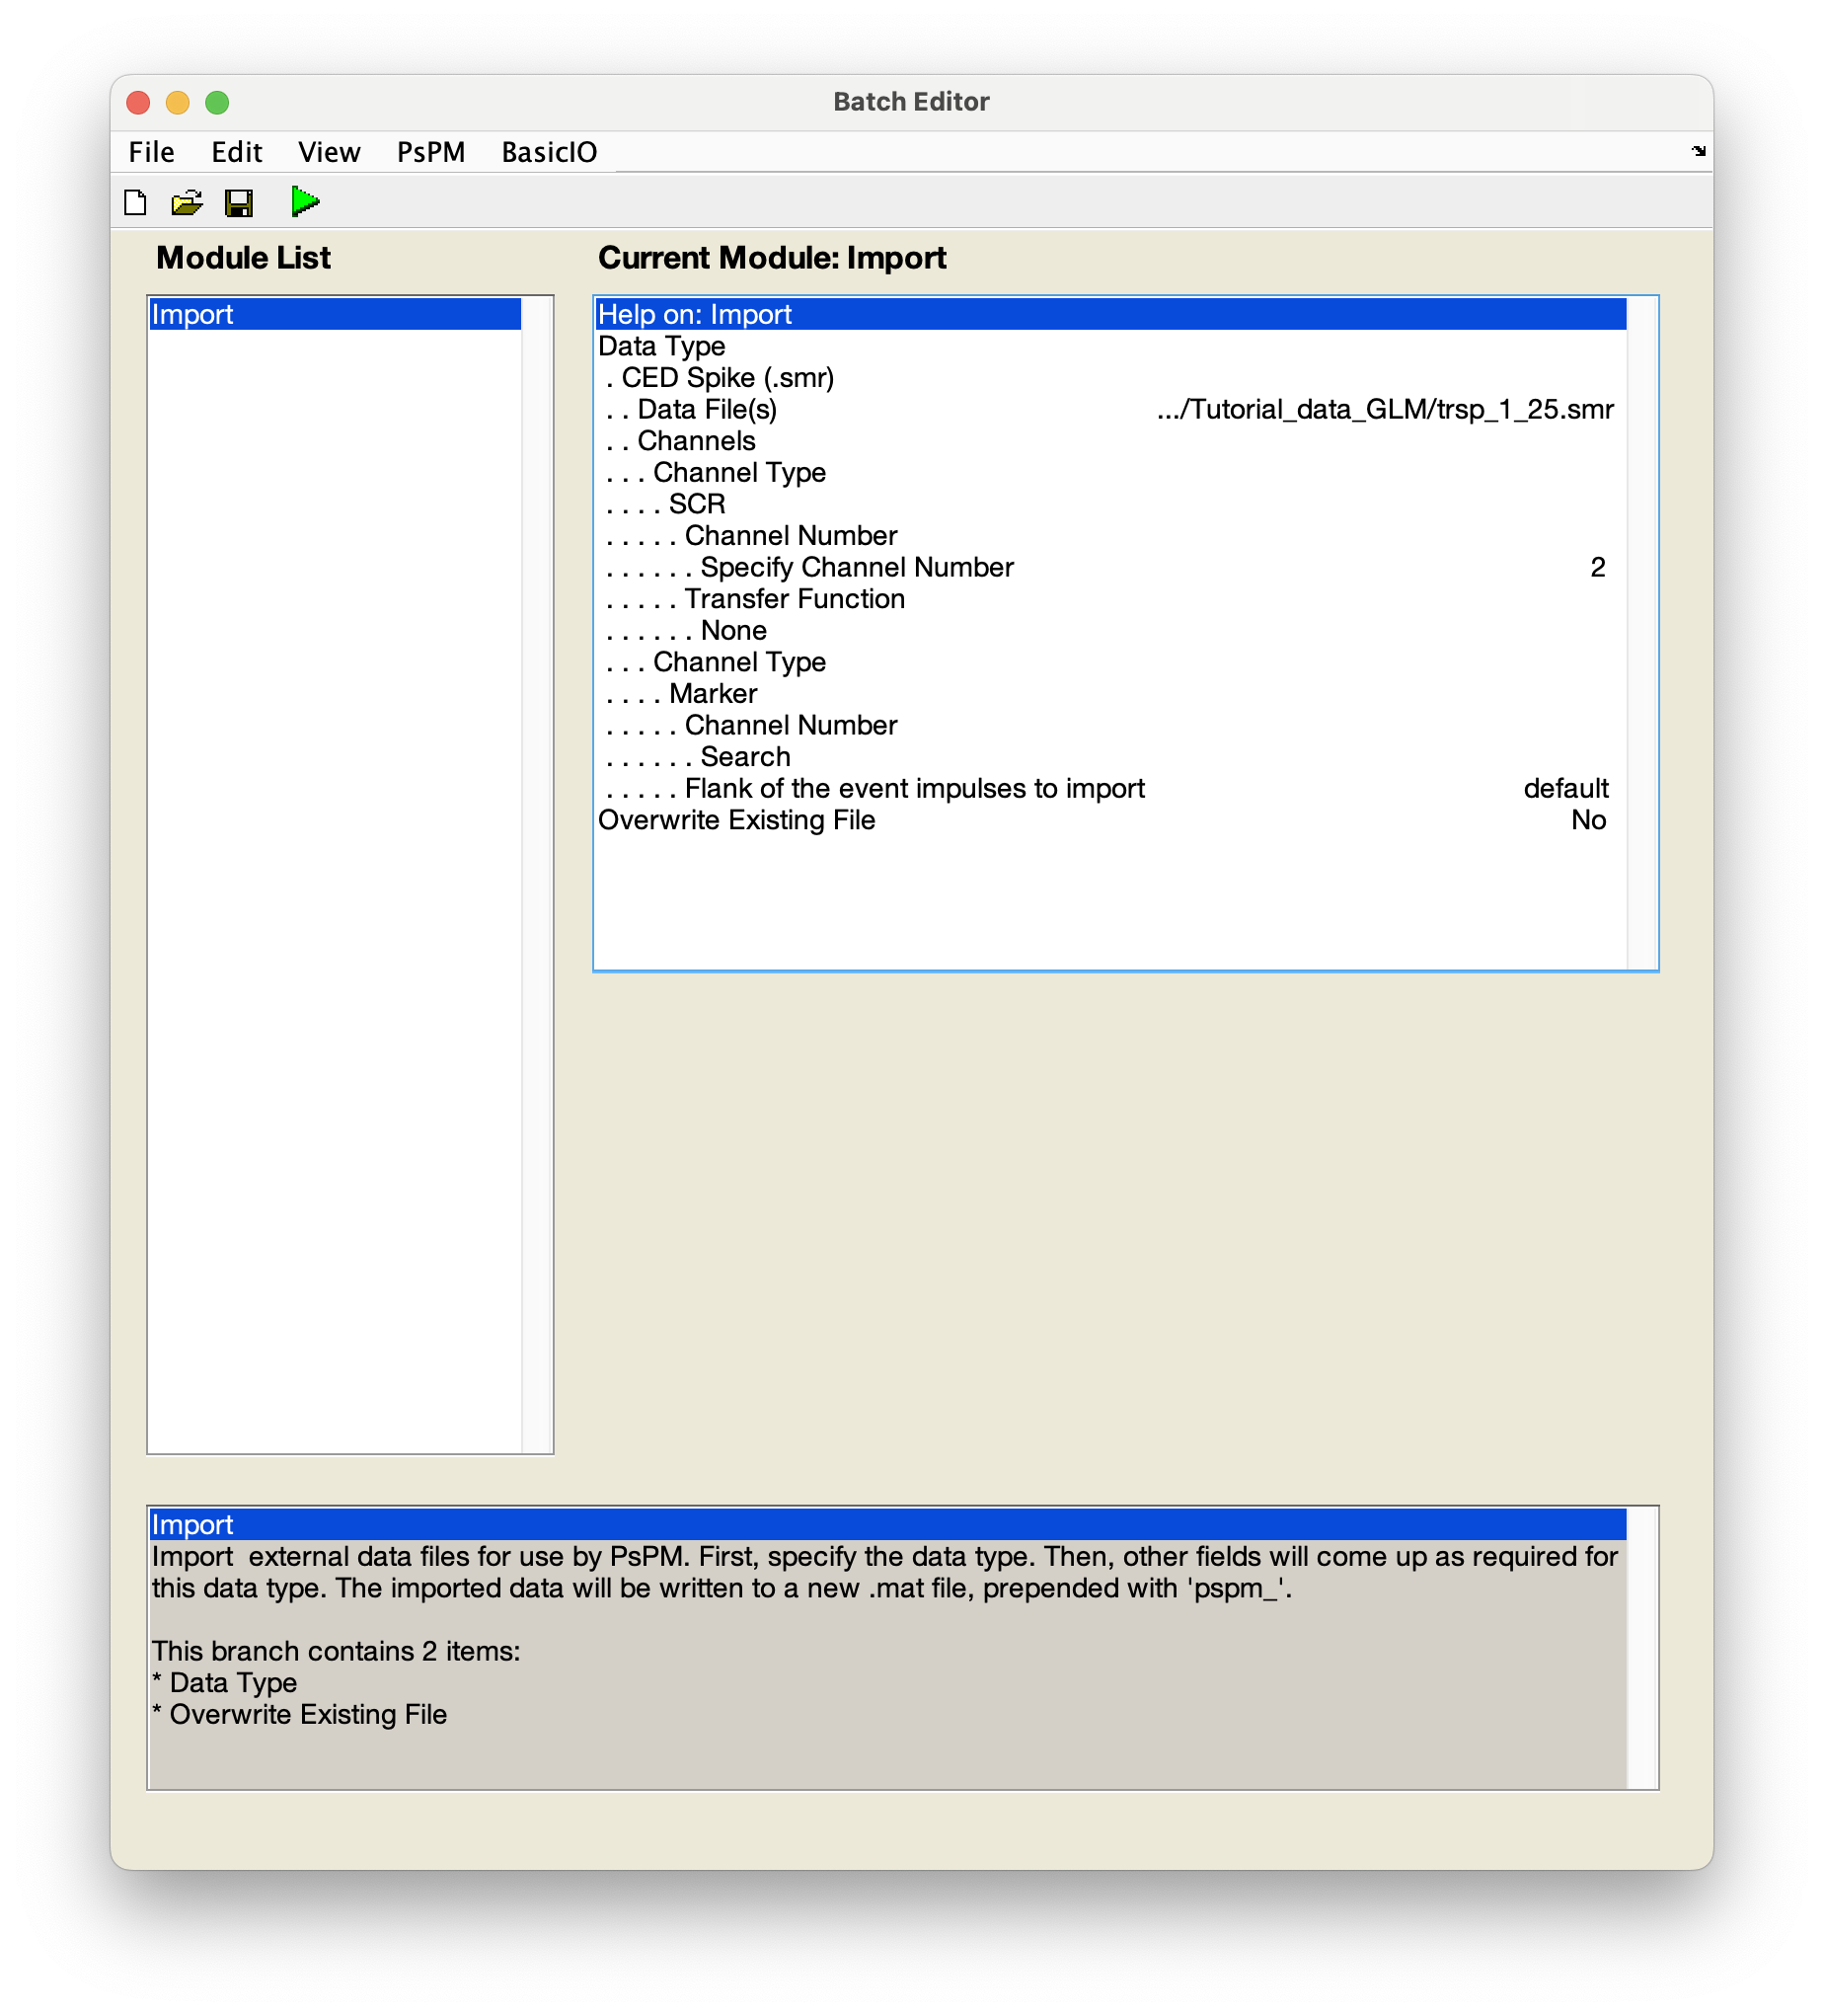
\includegraphics[scale=0.6]{Figures/YY1_import}\caption{Batch editor for importing raw SCR data.\label{fig:import}}
\end{figure}


\subsection{Trim}

Most of the time, the SCR recording is switched on some time before
the actual experiment starts and is switched off some time after it
ends. These parts of the time series may contain large artifacts from
subject motion, setting up the equipment, etc. Trimming excludes these
parts from the analyses.

\begin{figure}[H]
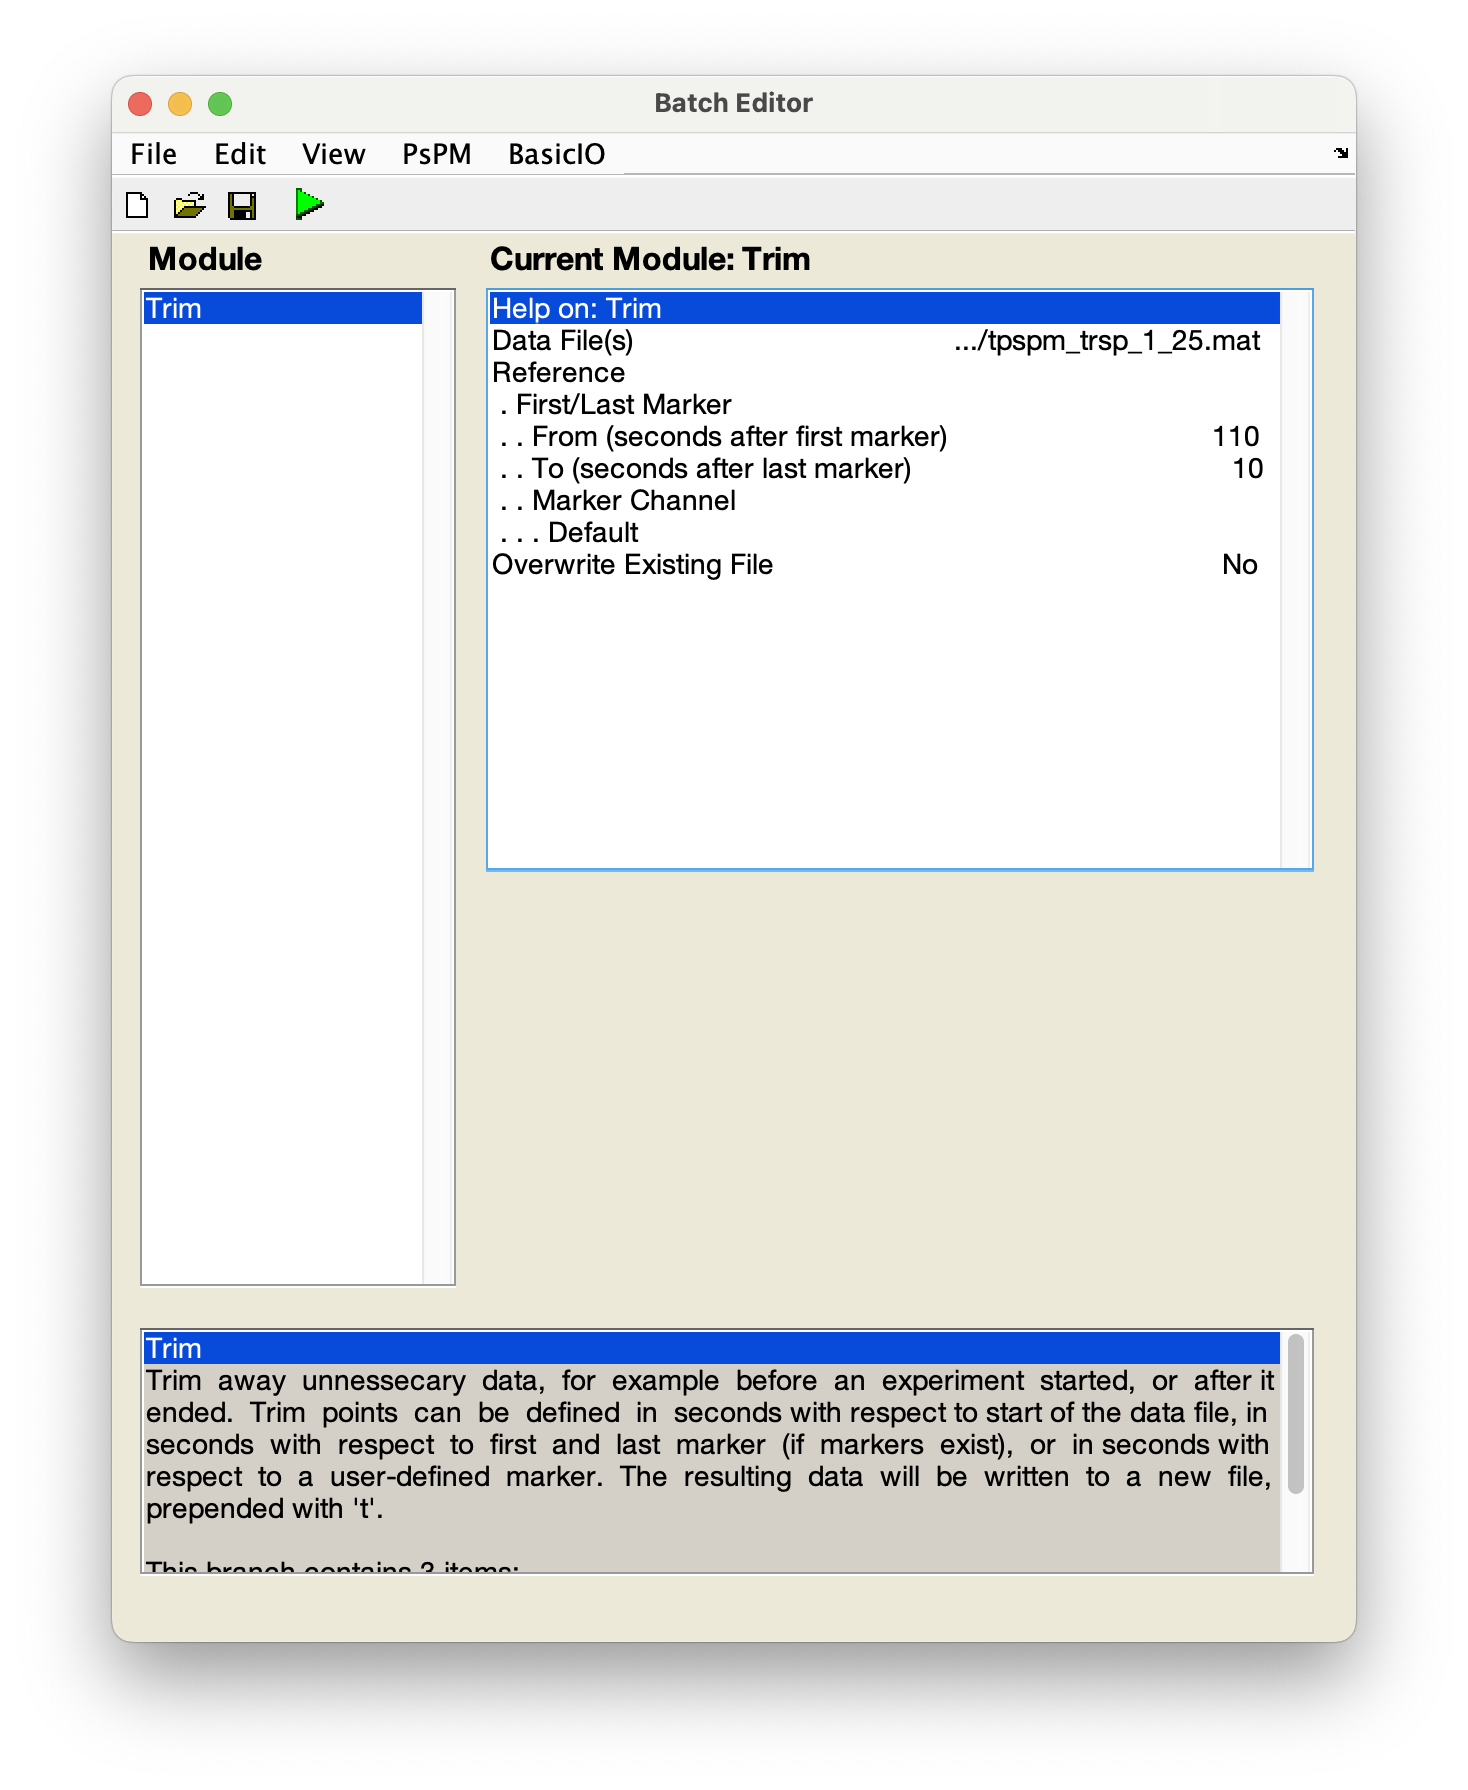
\includegraphics[scale=0.6]{Figures/YY2_trim}\caption{Batch editor for trimming SCR data.\label{fig:trim} }
\end{figure}

\begin{itemize}
\item In the batch editor go to \emph{PsPM $\rightarrow$ Data Preparation
$\rightarrow$Trim}.
\begin{itemize}
\item Select the currently imported file as Data File. Alternatively, you
can use the \emph{Dependency} button.
\end{itemize}
\item You can choose different References to specify how data should be
trimmed. Here, select \emph{First/Last Marker} and
\begin{itemize}
\item \emph{From (seconds after first marker)}: +110 (In the current data
set the first 2 minutes are a task-relevant baseline period and are
thus trimmed. Note that a positive number will delete at least the
first marker of the original data. Thus, make sure that a possible
specification of the First-Level takes this into account.)
\item \emph{To (seconds after first marker)}: 10 (The specified time window
should be large enough to completely include the last trial.)
\end{itemize}
\end{itemize}
You can also specify time points before the markers by using negative
numbers (see above). See Figure \ref{fig:trim} for a picture of the
final batch editor. Again, it is recommended to save the batch and
script for future use. Run the batch. A mat file with the name \texttt{tpspm\_trsp\_1\_25.mat}
will be created (i.e., a \textquotedblleft t\textquotedblright{} will
be prepended).

\subsection{First-Level}

Now, we specify the GLM on the first (i.e., the subject-specific)
level, estimating average responses per experimental condition (this
equivalent to averaging responses over trials in classical \textquotedbl peak
scoring\textquotedbl{} analysis, or to performing a first level analysis
in SPM).
\begin{itemize}
\item In the batch editor go to \emph{PsPM $\rightarrow$ First Level $\rightarrow$
SCR $\rightarrow$GLM}\textit{ for SCR}.
\item \emph{Model Filename}: This is the name of the resulting mat file
containing the GLM. Here, we call it \texttt{glm\_25}.
\item \emph{Output Directory}: The resulting mat file containing the GLM
will be saved in this folder.
\item \emph{Time Units} on which the specification of the conditions will
be based. Here, we want to analyze with respect to Markers.
\item \emph{Session(s)}: Similar to SPM, SCRalyze allows the specification
of multiple sessions per subject. Here, we only have one session.
\begin{itemize}
\item Add the trimmed data (\texttt{tpspm\_trsp\_1\_25.mat}) as Data File.
Alternatively, you can use the \emph{Dependency} button.
\item \emph{Missing Epochs} allows the specification of time periods which
you do not want to include in the analysis for example because they
contain corrupted data. In the example data set, there are no missing
epochs.
\item \emph{Data \& Design}: This option allows specifying the different
conditions of the experiment. You need to provide the information
when the different conditions started. This time information has to
be in the unit specified above (see \emph{Time Units}). In the current
data set, condition information is provided in Markers and is stored
in the mat file \texttt{trSP\_appraisal\_01\_25\_onsets\_1.mat}, which
you should select as \emph{Condition File}. When you open this file
in MATLAB, you will see that the file contains a 1x3 cell \textquotedblleft names\textquotedblright{}
and a 1x3 cell \textquotedblleft onsets\textquotedblright{} specifying
three conditions. The numbers in \textquotedblleft onsets\textquotedblright{}
correspond to the $n$th marker when the respective trial started.
\item \emph{Nuisance File} allows the inclusion of nuisance confounds such
as motion or respiration parameters. Here, we leave it empty.
\end{itemize}
\end{itemize}
\begin{figure}[H]
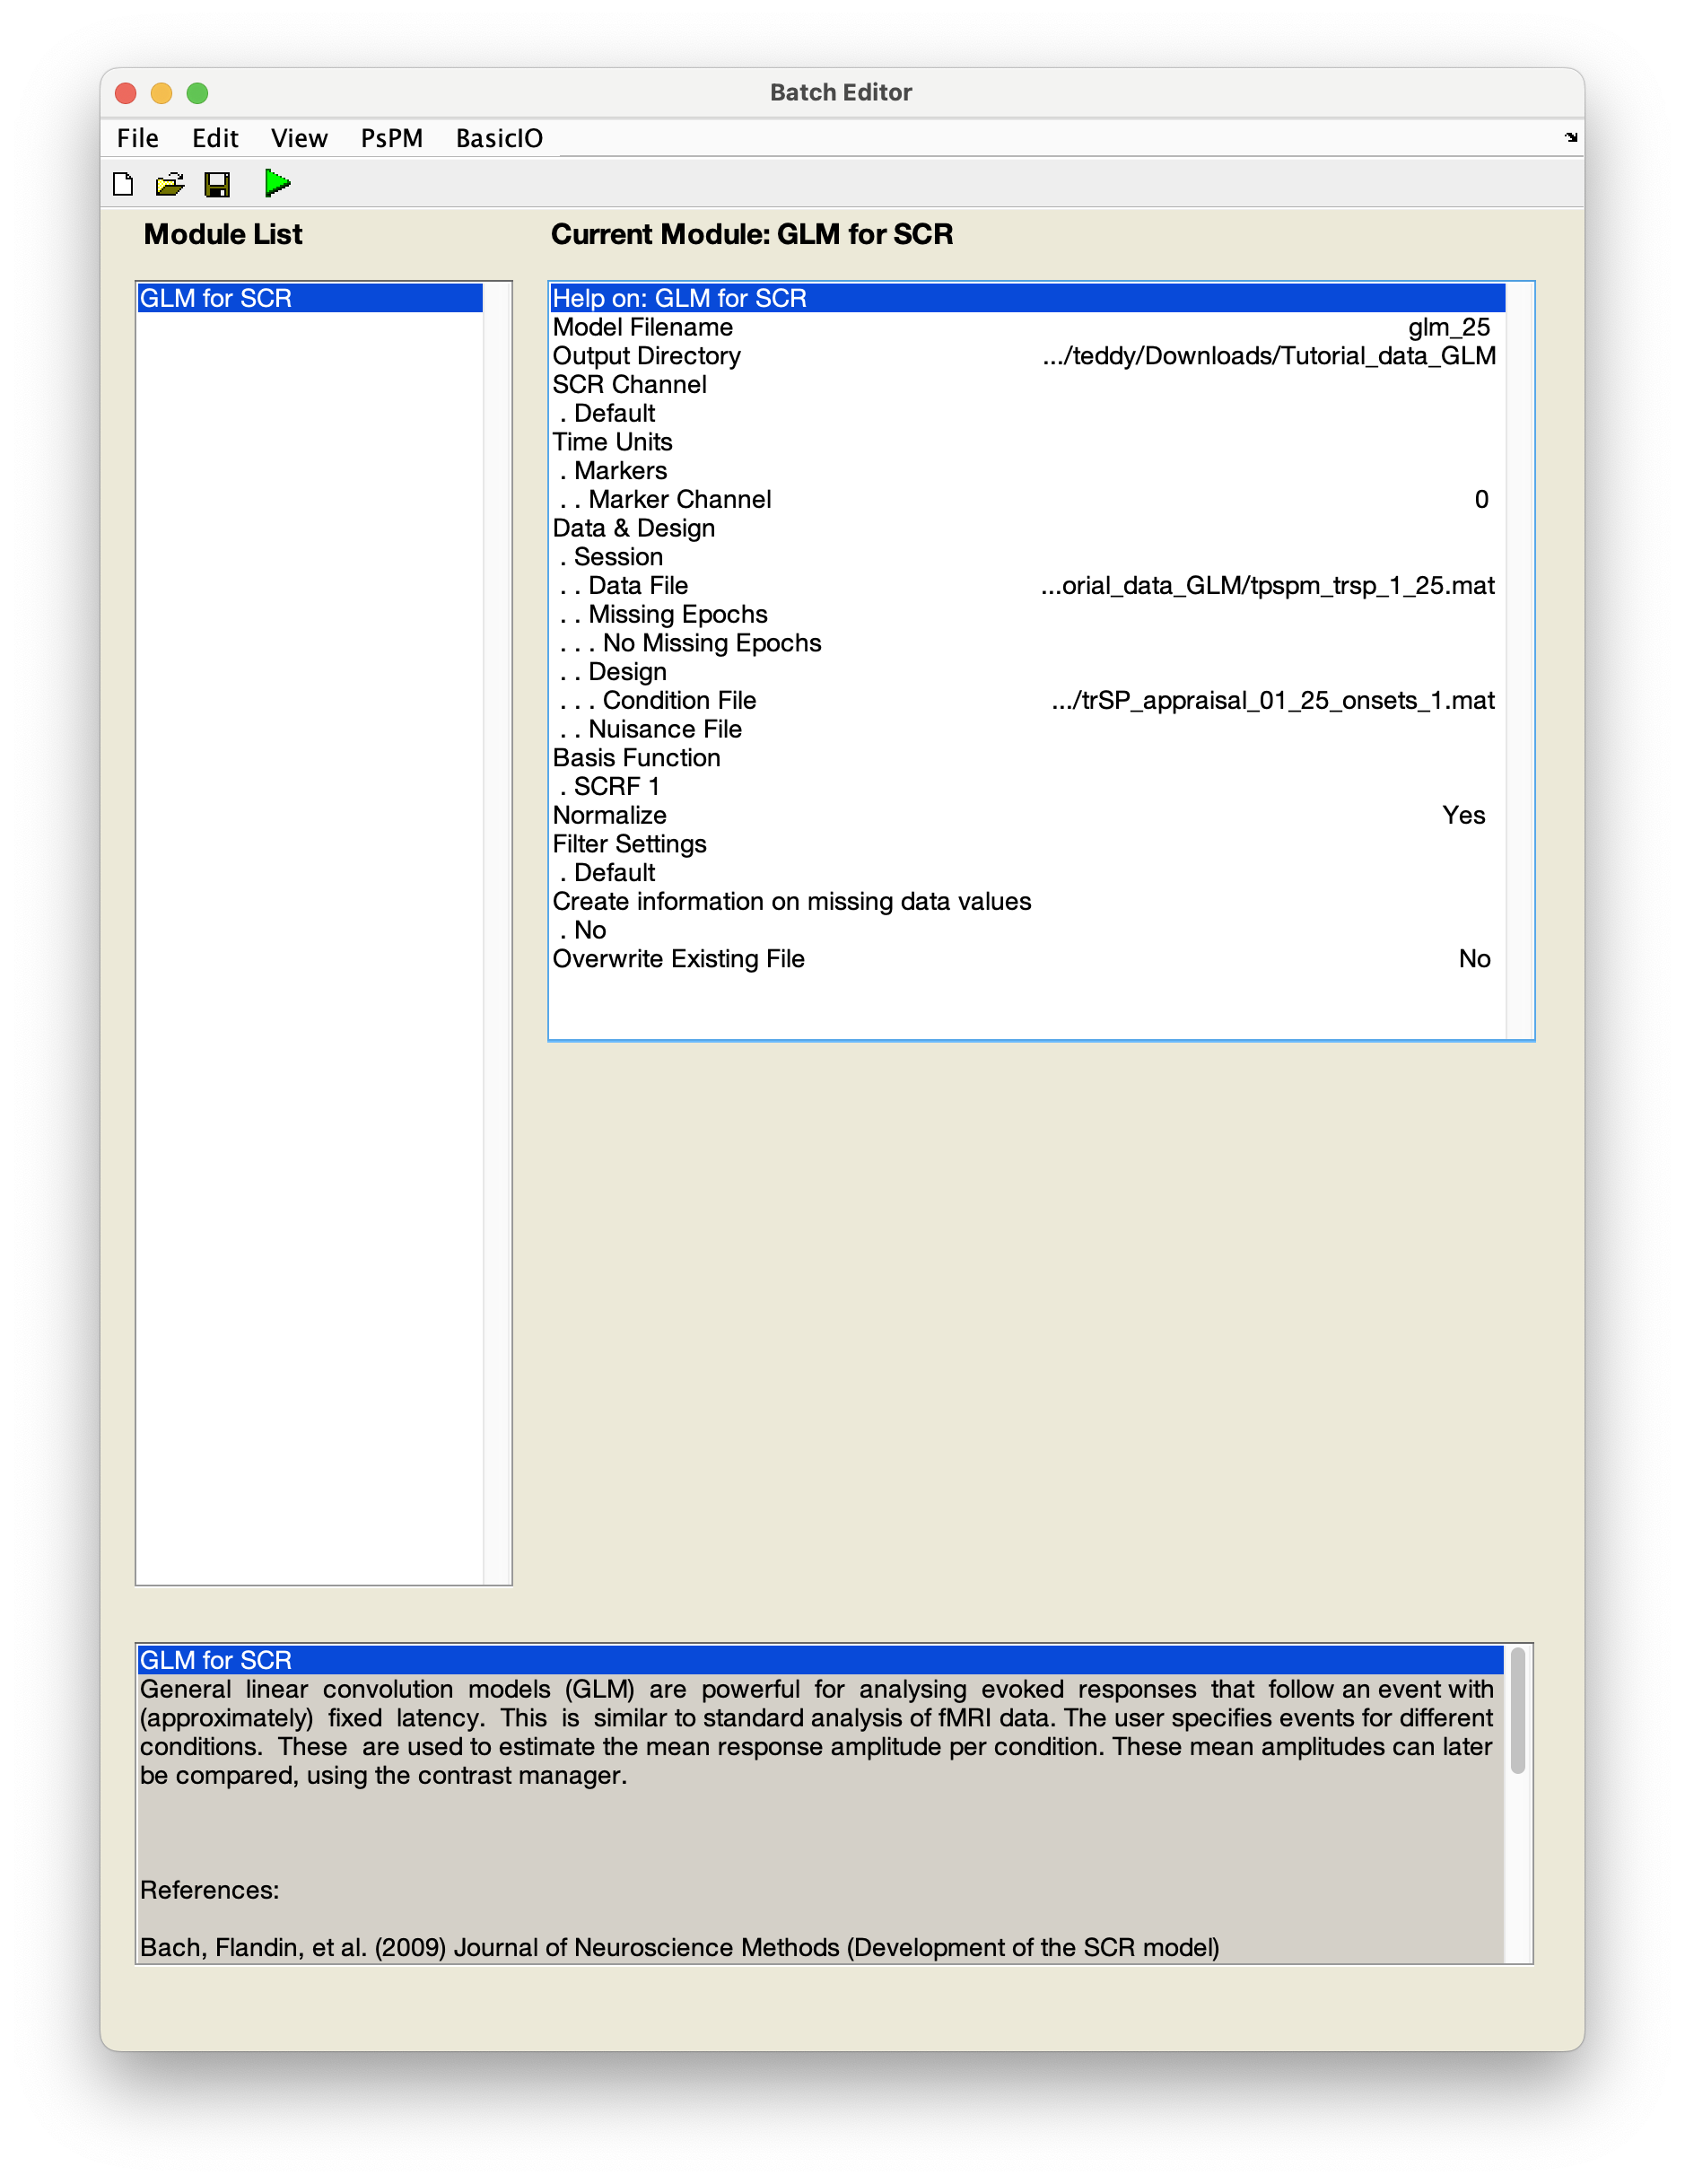
\includegraphics[scale=0.6]{Figures/YY3_glm}\caption{Batch editor for First-Level analysis. \label{fig:firstlevel}}
\end{figure}

\begin{itemize}
\item \emph{Basis Function}: We chose the default \emph{SCRF 1}, which is
the version with time derivative. The default basis set follows the
recommendations by \cite{Bach:2013aa}.
\item \emph{Normalize}: The design of the current data set is \textquotedblleft within-subjects.\textquotedblright{}
Therefore, we want to z-normalize the data.
\item \emph{Filter Settings}: We choose the default filter settings, which
follow the recommendations by \cite{Bach:2013aa}:
\begin{itemize}
\item first-order low-pass Butterworth filter with a cutoff frequency of
5 Hz
\item first-order high-pass Butterworth filter with a cutoff frequency of
0.05 Hz
\item Data are resampled to 10 Hz.
\item The filter direction is unidirectional.
\end{itemize}
\end{itemize}
See Figure \ref{fig:firstlevel} for a picture of the final batch
editor. Again, we recommend saving the batch and script for future
use. Run the batch. A mat file with the specified name will be created
in the specified folder. 

\subsection{Review First-Level Model}

You can have a look at plots related to the first-level model in the
batch editor.
\begin{itemize}
\item In the batch editor go to \emph{PsPM $\rightarrow$ First Level $\rightarrow$
Review First-level Model}.
\item Specify the Model file that you want to review. Select the mat file
containing the GLM (e.g., \texttt{glm\_25.mat}).
\item The \emph{Model Type} is of course GLM in the current example. You
can set the following options to get different types of information:

\begin{enumerate}
\item \emph{Design matrix}: On the x-axis, you see the number of regressors
in the model. Here we have specified 7 regressors in total. On the
y-axis, you see the time course of the experiment. Note that there
are 7 regressors because the specification for the \emph{Basis Function}
was \emph{SCRF with time derivative}. That is, 3 (conditions times)
x 2 (basis functions) + 1 (constant) = 7 regressors. You can see that
neutral and aversive are intermixed and fall into three blocks. See
Figure \ref{fig:review1}.
\item \emph{Orthogonality}: On the x- and y-axes you see the specified regressors.
Regressor names are additionally specified along the y-axes. The plot
depicts the collinearity between regressors. See Figure \ref{fig:review2}.
\item \emph{Predicted \& Observed}: You see the model fit including the
observed response over the whole time series, which you can visually
compare to the predicted time series by the specified model. Note
that the predicted data will never follow the observed data very closely,
because we estimated the average response per condition which will
deviate from the response in each individual trial. See Figure \ref{fig:review3}.
\item \emph{Regressor names}: The names of the regressors as specified in
the \emph{Conditions File} under \emph{Data \& Design} are written
to the MATLAB command window. The labels bf 1 and bf 2 refer to the
two used basis functions (\emph{SCRF with time derivative}).
\item \emph{Reconstructed}: Here you see the estimated responses per condition
for the first basis function. These are estimates of the true responses
which contain noise. The noise term can be negative but if all estimated
responses across an entire group are negative it is a good idea to
look for confounds or correlations in the design. See Figure \ref{fig:review4}.
\end{enumerate}
\end{itemize}
\begin{figure}[H]
\includegraphics[scale=0.5]{Figures/YY41_review}\caption{Design matrix for sample participant. On the x-axis, you see the number
of regressors in the model. There are 7 regressors (i.e., 3 (conditions
times) x 2 (basis functions) + 1 (constant)). \label{fig:review1}}
\end{figure}

\begin{figure}[H]
\includegraphics[scale=0.35]{Figures/YY42_review}\caption{Design orthogonality plot for sample participant. On the x- and y-axes
you see the 7 specified regressors. \label{fig:review2}}

\end{figure}

\begin{figure}[H]
\includegraphics[scale=0.35]{Figures/YY43_review}\caption{Model fit for sample participant. You see the observed response and
the predicted response according to the model over the whole time
series. \label{fig:review3} }

\end{figure}

\begin{figure}[H]
\includegraphics[scale=0.35]{Figures/YY44_review}\caption{Estimated responses per condition for sample participant. You see
the estimated responses per condition for the first basis function.
\label{fig:review4}}

\end{figure}


\subsection{First-Level Contrast Manager}

We want to compare the difference between aversive and neutral pictures
across participants (i.e., on the second level). This can be tested
in a paired t-test. A paired t-test is a one-sample t-test on difference
values between two conditions. The contrast manager allows you to
compute such difference values, for each participant (i.e., on the
first level).
\begin{itemize}
\item In the batch editor go to \emph{PsPM $\rightarrow$ First-Level $\rightarrow$
First-Level Contrasts}.
\item \emph{Model File(s)}: Select the mat file containing the GLM (here
\texttt{glm\_25.mat}).
\item \emph{Stats type}: You can choose between 3 different options to set
up the contrasts. Here, we choose the option Condition, which specifies
contrasts formulated in terms of conditions and automatically uses
only the first basis function (i.e., without derivatives).
\item \emph{Contrast}

\begin{itemize}
\item \emph{Contrast Name}: Chose a name so that you can easily refer to
the contrast (e.g., aversive>neutral)
\item \emph{Contrast Vector}: Specify a vector of the contrast you want
to test for. Here, we are interested in the difference between aversive
and neutral pictures, i.e., the first and the second condition. Therefore,
specify the vector {[}-1, 1, 0{]}. You could also leave out the last
zero because trailing zeros are automatically appended. (But you could
not leave out the first zero in a contrast such as {[}0 -1 1{]}.)
\end{itemize}
\end{itemize}

\subsection{Export Statistics}

You can use this functionality to export all necessary parameters
on the screen or into an extra file, which allows you to analyze the
data in the statistics program of your choice. For details see \emph{PsPM
$\rightarrow$ First Level} \emph{$\rightarrow$ Export Statistics}.

\subsection{Adapting scripts for multiple participants and second-level analyses }

For didactic purposes, we have so far only considered one participant.
But in most experiments, you want to analyze data from multiple subjects
(i.e., a second-level analysis). For a description on how to do this
see Chapters \ref{sec:Adapting-scripts-for} and \ref{sec:Second-level-Contrast-Manager}.
You can find a script that runs the above described analyses for multiple
participants at \href{http://pspm.sourceforge.net}{pspm.sourceforge.net}
(import\_trim\_glm\_contr\_job\_loop). 

\section{Non-linear SCR tutorial: Delay fear conditioning data\label{sec:Delay-fear-conditioning}}

The example data set comprises SCR data from 20 participants, with
40 trials each, which can be downloaded from \href{https://bachlab.github.io/PsPM/software/}{https://bachlab.github.io/PsPM/software/}
together with the result files of the model inversion. Participants
underwent a differential delay fear conditioning paradigm where coloured
circles were presented for 4 seconds each. Either the blue or orange
coloured circles (balanced over participants) were probabilistically
paired with an electric stimulation (unconditioned stimulus, US) that
coterminated with the stimulus (conditioned stimulus, CS+) while the
CS- were always presented alone.

Presenting the CS+ causes phasic sympathetic arousal in anticipation
of an electric shock. This anticipatory reaction typically occurs
with an unknown and variable latency after stimulus onset. For such
cases, a GLM should not be used because it assumes that sympathetic
arousal follows the stimulus with a fixed latency. In contrast, the
non-linear model allows estimating (i) a variable onset within a user-specified
time window and (ii) a variable duration of a sympathetic response.
Additionally, the non-linear model includes estimation of spontaneous
fluctuations that occur between trials.

In this tutorial, the non-linear model is estimated. The estimated
parameters can then be used to test the within-subject hypothesis
that the sympathetic arousal between CS+ and CS- are different on
a group level.

\subsection{Setup the Non-Linear Model}

In this step you prepare the model estimation. For this, you need
to provide timing information about the experimental events which
can either be entered manually or as a Matlab file. For large numbers
of events as in this experiment, a timing file can easily be created
using a few lines of Matlab code. Here we use timing information saved
in the trimmed PsPM file. In this file, a trigger was saved at every
CS onset. For timing information from other sources, the code has
to be adapted accordingly. Go to the Matlab command window and enter
the following lines, but replace \texttt{{[}insert path!{]}} by the
correct path where the filtered SCR data from \href{http://pspm.sourceforge.net}{pspm.sourceforge.net}
is saved on your hard drive, e.g. \texttt{C:\textbackslash PsPM\_Tutorial\textbackslash nonlinear\textbackslash}.

\begin{lstlisting}
data_path = [insert path!]; % set the correct PsPM file path here!

p = 1; % the first participant
SOA = 3.5; % delay between CS and US onset in seconds

% load events of CS onsets from trimmed scr data
pname = fullfile(data_path,sprintf('tpspm_s%i.mat',p))
[sts, infos, data, filestruct] = pspm_load_data(pname,'events');

CS_onset = data{1, 1}.data; % recorded triggers of CS onset in seconds
US_onset = data{1, 1}.data + SOA; % US starts 3.5 seconds after CS

% variable latency for CS response between CS onset and US onset/omission
events{1} = [CS_onset US_onset]; % define an interval of 3.5 seconds for each trial
% constant onset for US response
events{2} = US_onset;

save(fullfile(data_path,sprintf('event_timings_s%i.mat',p)),'events')
\end{lstlisting}

\noindent \begin{flushleft}
The resulting file \texttt{event\_timings\_s1.mat} contains the variable
events with two cells.
\par\end{flushleft}
\begin{itemize}
\item The first cell \emph{events\{1\}} is a 40 x 2 matrix with the onset
and offset of a time window for each trial in which we expect the
response to the CS (both CS+ and CS- are treated the same here). We
expect the response to the CS to occur with a variable onset in time.
Note that the window for the CS response ends when the US starts (or
is omitted), i.e. after 3.5 seconds.
\item The second cell \emph{events\{2\}} is a 40 x 1 vector that marks the
onset of the electrical stimulation. For this event we expect an evoked
response with constant latency after US occurrence. Importantly, we
provide timings \emph{both for the occurrence and the omission of
the US}. Modelling an unconditioned response in all trials is necessary
to get unbiased estimates for the CS responses. In general, the trial
structure should always be the same for all trials, across experimental
conditions.
\end{itemize}
Now the non-linear model estimation can be set up (Figure \ref{fig:Prepare-a-batch}).

\begin{figure}[H]
\includegraphics[scale=0.65]{Figures/Batch_nonlinear}

\caption{Prepare a batch to set up a non linear model for SCR analysis.\label{fig:Prepare-a-batch}}
\end{figure}

\begin{itemize}
\item In the batch editor go to \emph{PsPM }$\rightarrow$\emph{ First Level
}$\rightarrow$\emph{ SCR $\rightarrow$ Non-Linear Model}
\item \emph{Model Filename}: dcm\_s1
\item \emph{Output Directory}: Specify a folder where the model will be
saved
\item \emph{Chan}nel: Default
\item \emph{Data \& Design:$\rightarrow$New: Session}

\begin{itemize}
\item \emph{Data File}: choose tscr\_s1.mat from your hard drive
\item \emph{Design$\rightarrow$Timing File$\rightarrow$}Select the previously
created \texttt{event\_timings\_s1.mat} which was saved to your scr
folder
\item \emph{Condition names: New Condition} here we can define conditions
that each trial belongs to. Create three new conditions. Note that
we split CS+ trials in reinforced (CS+|US+) and non-reinforced (CS+|US-)
trials because CS+|US+ trials are excluded from some analyses.
\begin{itemize}
\item \emph{Condition}

\begin{itemize}
\item \emph{Name: CS+|US-}
\item \emph{Index: 6 7 11 14 16 18 26 29 38 40}
\end{itemize}
\item \emph{Condition}

\begin{itemize}
\item \emph{Name: CS+|US+}
\item \emph{Index: 13 17 19 20 21 24 28 31 32 37}
\end{itemize}
\item \emph{Condition}

\begin{itemize}
\item \emph{Name: CS-}
\item \emph{Index: 1 2 3 4 5 8 9 10 12 15 22 23 25 27 30 33 34 35 36 39}
\end{itemize}
\end{itemize}
\end{itemize}
\item \emph{Display Options}

\begin{itemize}
\item \emph{Display Progress Window}: If you plan to run the estimation
in the background, you can turn off the progress window with this
option
\end{itemize}
\item \emph{For the remaining fields you can keep the default settings}
\end{itemize}
Save the batch and script as \texttt{batch\_model\_s1.m} and press
run. A window will be displayed that shows the progress of model estimation
for each trial. The estimation for an entire session takes several
minutes depending on your system. The file \texttt{dcm\_s1.mat} will
be created. If you want to, you can review the first-level model by
clicking \emph{Review model} in the PsPM user interface. In the new
window (Figure \ref{fig:Use-Review-Model}) add the non-linear model
\texttt{dcm\_s1.mat} and choose \emph{Display All trials for one session}.
A graphics window (Fig X) will display the original data (blue) together
with the model estimation (green).

\begin{figure}[H]
\includegraphics[scale=0.5]{Figures/Review_1stmodel1.PNG}

\caption{Use \emph{Review Model} to inspect parameter estimation for one or
multiple trials.\label{fig:Use-Review-Model}}
\end{figure}


\subsection{First-level Contrasts}

In this step you specify the hypothesis that a CS+ elicits a stronger
sympathetic arousal than a CS- for an individual participant by providing
a contrast weight vector.
\begin{itemize}
\item In the batch editor go to \emph{PsPM$\rightarrow$First Level$\rightarrow$First-level
Contrasts}
\item \emph{Model File(s):} Select \texttt{dcm\_s1.mat}
\item \emph{Specify Contrasts on Datatype: param}
\item \emph{Contrasts: New Contrast}

\begin{itemize}
\item \emph{Contrast }

\begin{itemize}
\item \emph{Name: Fear Learning}
\item \emph{Contrast Vector: -1 -1 -1 -1 -1 2 2 -1 -1 -1 2 -1 0 2 -1 2 0
2 0 0 0 -1 -1 0 -1 2 -1 0 2 -1 0 0 -1 -1 -1 -1 0 2 -1 2} Note: A weight
of +2 is assigned to the CS+|US- because we have twice as many CS-
and the contrast vector has to sum up to zero.
\item \emph{Name: Electric Stimulation} We include this contrast optionally
to check if the electrical stimulation caused an increase in sympathetic
arousal which is a premise for successful fear conditioning.
\item \emph{Contrast Vector: -1 -1 -1 -1 -1 -1 -1 -1 -1 -1 -1 -1 3 -1 -1
-1 3 -1 3 3 3 -1 -1 3 -1 -1 -1 3 -1 -1 3 3 -1 -1 -1 -1 3 -1 -1 -1}
\end{itemize}
\end{itemize}
\item \emph{Delete: existing contrasts: No (default)}
\end{itemize}
Save the batch and script as \texttt{batch\_contrast\_s1.m} and press
run. The model file of participant s1 now contains the contrast that
can be forwarded to a statistical test on group level. Preparing analyses
for more than one scr file is explained in Chapter \ref{sec:Adapting-scripts-for}.

\subsection{Exporting statistics}

PsPM provides basic tools for statistical analysis on the estimates
of the non-linear model. Alternatively you can export the results
as a text file to use them in different software applications.
\begin{itemize}
\item In the batch editor go to SCR$\rightarrow$First Level$\rightarrow$Export
Data
\item \emph{Model File(s): }Select \emph{dcm\_s1.mat}
\item \emph{Specify Export on Datatype: param}
\item \emph{Target}

\begin{itemize}
\item \emph{Filename }Enter\emph{ }\texttt{dcm\_s01}
\end{itemize}
\item \emph{Specify Delimiter for Output File}

\begin{itemize}
\item \emph{Semicolon}
\end{itemize}
\end{itemize}
The text file will be saved to Matlab\textquoteright s current working
directory.

\section{Adapting scripts for multiple participants\label{sec:Adapting-scripts-for}}

In most experiments, you want to analyze data from multiple subjects,
which implies that you have to repeat model estimation several times.
There are two simple strategies to make this easier.
\begin{itemize}
\item Use dependencies: You can specify all steps for one subject in one
go. At some points, you need to specify a file from a previous step
(e.g., when trimming you need the file containing the imported data).
In these cases, you can use the button \textquotedblleft Dependency\textquotedblright{}
to specify the corresponding file, but make sure the number of output
files of the preceding module corresponds with the allowed number
of input files for this module.
\item Loop over participants in the script: You can easily adapt the scripts
for many subjects by including a loop and adapting the file names.
This is independent of whether or not you use dependencies. To show
you how this works, see the examples below.
\end{itemize}

\subsection{Importing and trimming data}

Here, we create an example script for importing and trimming data.
We chose these steps since they are required in all types of analysis.
The current example is based on the Appraisal dataset described in
Chapter \ref{sec:tutorial_GLM}.
\begin{itemize}
\item In the batch editor specify all parameters in PsPM $\rightarrow$
Data Preparation $\rightarrow$ Import.
\item You do not need to specify the SCR Data File. This will later be put
in the script that loops over subjects.
\item In the batch editor specify all parameters in PsPM $\rightarrow$
Data Preparation $\rightarrow$ Trim.
\item Use the dependency button to select the imported Data File.
\item Save batch and script.
\item Open the saved job script (e.g., \texttt{batch\_import\_trim\_job.m})
and build a loop around the lines of code that were saved. In this
loop, create a subject-specific filename (and make sure to include
the whole path to the files in the variable data\_path).
\end{itemize}
\noindent 
\begin{lstlisting}
data_path = [insert path!];

for p = 25:39; % participants
% load participant-specific raw data
spike.datafile = {fullfile(data_path,sprintf('trsp_1_%i.smr',p))};
spike.importtype{1}.scr.chan_nr.chan_nr_spec = 2;
spike.importtype{1}.scr.transfer.none = true;
spike.importtype{2}.marker.chan_nr.chan_nr_spec = 0;
matlabbatch{1}.pspm{1}.prep{1}.import.datatype.spike = spike;
matlabbatch{1}.pspm{1}.prep{1}.import.overwrite = false;
matlabbatch{2}.pspm{1}.prep{1}.trim.datafile(1) = ...
cfg_dep('Import: Output File', substruct('.', ... 
'val', '{}',{1}, '.','val', ...
'{}',{1}, '.','val', '{}',{1}), substruct('()',{':'}));
matlabbatch{2}.pspm{1}.prep{1}.trim.ref.ref_mrk.from = 110;
matlabbatch{2}.pspm{1}.prep{1}.trim.ref.ref_mrk.to = 10;
matlabbatch{2}.pspm{1}.prep{1}.trim.ref.ref_mrk.mrk_chan.chan_def = 0;
matlabbatch{2}.pspm{1}.prep{1}.trim.overwrite = false;

% run batch
pspm_jobman('initcfg');
pspm_jobman('run', matlabbatch);

end
\end{lstlisting}

\noindent Run the script. The folder \texttt{data\_path} now contains
trimmed scr files for all subjects.

\subsection{Inverting non-linear models}

Here we adapt the model inversion from Chapter \ref{sec:Delay-fear-conditioning}
to multiple subjects. We use similar loops as above to create timing
files and PsPM batches.

First, open the MATLAB script that created the timing file \texttt{event\_timings\_s1.mat}
and construct a loop around it for subjects 2 to 20. Execute the script
to obtain files containing timing information for subjects 2 to 20.
Alternatively you can use the timing files for subjects 2 to 20 downloaded
from \href{http://pspm.sourceforge.net}{pspm.sourceforge.net}.

Next, open the saved job script (e.g., \texttt{batch\_model\_s1\_job.m})
created in Chapter \ref{sec:Delay-fear-conditioning} and build a
loop around the lines of code that were saved. Make sure to include
the whole path to the files in the variable \texttt{data\_path}. You
can use the following code as guideline.\\
\begin{lstlisting}
% set the path where you saved the scr data files
data_path = [insert path!];

% set the path where you saved the model file of participant 1
model_path = [insert path!]; % initiate PsPM pspm_init % loop through participants 2 to 20

% initialize PsPM
pspm_init
pspm_jobman('initcfg')

for p = 2:20

clear matlabbatch dcm
dcm.modelfile = ['dcm_s' num2str(p)];
dcm.outdir = {model_path};
dcm.chan.chan_def = 0;
dcm.session.datafile = ...
{fullfile(data_path,['tpspm_s' num2str(p) '.mat'])};
dcm.session.timing.timingfile = ...
{fullfile(data_path,['event_timings_s' num2str(p) '.mat'])};
dcm.session.condition(1).name = 'CS+|US-';
dcm.session.condition(1).index = [6 7 11 14 16 18 26 29 38 40];
dcm.session.condition(2).name = 'CS+|US+';
dcm.session.condition(2).index = [13 17 19 20 21 24 28 31 32 37];
dcm.session.condition(3).name = 'CS-';
dcm.session.condition(3).index = ...
[1 2 3 4 5 8 9 10 12 15 22 23 25 27 30 33 34 35 36 39];
dcm.data_options.norm = 0;
dcm.data_options.filter.def = 0;
dcm.resp_options.crfupdate = 0;
dcm.resp_options.indrf = 0;
dcm.resp_options.getrf = 0;
dcm.resp_options.rf = 0;
dcm.inv_options.depth = 2;
dcm.inv_options.sfpre = 2;
dcm.inv_options.sfpost = 5;
dcm.inv_options.sffreq = 0.5;
dcm.inv_options.sclpre = 2;
dcm.inv_options.sclpost = 5;
dcm.inv_options.ascr_sigma_offset = 0.1;
dcm.disp_options.dispwin = 0;
dcm.disp_options.dispsmallwin = 0;

matlabbatch{1}.pspm{1}.first_level{1}.scr{1}.dcm = dcm;

% run batch
pspm_jobman('run', matlabbatch);

end
\end{lstlisting}

\noindent Similarly to the previous step, the batch of the first-level
Contrast of participant 1 is adapted to participants 2 to 20. Run
the following code in MATLAB, but replace\texttt{ {[}insert path!{]}}
with the path on your hard drive where you saved \texttt{dcm\_s1.mat}:\\
\begin{lstlisting}
% set the path where you saved the estimated non-linear model
model_path = [insert path!];

% initialize PsPM
pspm_init
pspm_jobman('initcfg')

% loop through participants 2 to 20
for p = 2:20

clear matlabbatch
matlabbatch{1}.pspm{1}.first_level{1}.contrast.modelfile = ...
{fullfile(model_path,['dcm_s' num2str(p) '.mat'])};
matlabbatch{1}.pspm{1}.first_level{1}.contrast.datatype = 'param';
matlabbatch{1}.pspm{1}.first_level{1}.contrast.con(1).conname = 'Fear Learning';
matlabbatch{1}.pspm{1}.first_level{1}.contrast.con(1).convec = ...
[-1 -1 -1 -1 -1 2 2 -1 -1 -1 2 -1 0 2 -1 2 0 2 ...
0 0 0 -1 -1 0 -1 2 -1 0 2 -1 0 0 -1 -1 -1 -1 0 2 -1 2];
matlabbatch{1}.pspm{1}.first_level{1}.contrast.con(2).conname = ...
'Electric Stimulation';
matlabbatch{1}.pspm{1}.first_level{1}.contrast.con(2).convec = ...
[-1 -1 -1 -1 -1 -1 -1 -1 -1 -1 -1 -1 3 -1 -1 -1 ...
3 -1 3 3 3 -1 -1 3 -1 -1 -1 3 -1 -1 3 3 -1 -1 -1 -1 3 -1 -1 -1];
matlabbatch{1}.pspm{1}.first_level{1}.contrast.deletecon = true;

% run batch manually
pspm_jobman('run', matlabbatch);

end
\end{lstlisting}

\noindent Run the script. The statistics for each contrast are now
added to the model file.

\section{Second-level Contrast Manager\label{sec:Second-level-Contrast-Manager}}

In most cases, we want to compare the difference between conditions
across participants on a group level (i.e., the second level in a
hierarchical model). Each participant represents one data point that
goes into a one sample t-test.

Below we demonstrate how to set-up Second-level contrasts for GLM
and non-linear models.

\subsection{GLM}

For the appraisal data of Chapter \ref{sec:tutorial_GLM}.

\subsubsection{Define Second-Level Model}
\begin{itemize}
\item In the batch editor go to \emph{PsPM$\rightarrow$Second Level$\rightarrow$Define
Second-Level Model}.

\begin{itemize}
\item \emph{Test Type: One Sample T-Test}
\item \emph{Model File(s)}: Select the model files from all participants
\item \emph{Output Directory:} Choose a location to save the group result
\item \emph{Filename for Output Model}: Chose a name so that you can easily
refer to the contrast
\item \emph{Define Contrast: Read from First Model File}: Choose \emph{All
Contrasts}. This will select the contrast(s) that we created in the
first level (i.e., in our case aversive>neutral)
\end{itemize}
\end{itemize}

\subsubsection{Report Second-Level Results}
\begin{itemize}
\item In the batch editor go to \emph{PsPM $\rightarrow$Second Level$\rightarrow$Report
Second-Level Results}.

\begin{itemize}
\item \emph{Model File}: Select the second level model file that you created
in the previous step.
\item \emph{Contrast Vector}: Leave empty because we want all contrasts
to be reported.
\end{itemize}
\end{itemize}
Run the batch. A figure appears that shows you a bar graph of the
mean of the parameter estimates and the statistics will be printed
to the MATLAB command window.

\subsection{Non-linear models}

Here, we test the difference in anticipatory sympathetic arousal elicited
by a CS+ vs CS- on a group level (see Chapter \ref{sec:Delay-fear-conditioning}).
As a supplementary hypothesis we want to check if the US+ indeed elicited
a stronger response than the US-. From the 1st level contrast, eight
statistics were generated for each model file. Use the \emph{Review
Model} utility from the PsPM main GUI to get a list of all contrasts.
In the \emph{First Level Review Manager}, click on \emph{Add Model},
choose any model file created previously and press \emph{Done}. Now
press the Show button next to \emph{Contrast names in command window}
(Figure \ref{fig:FLRM2}) to get a list of all contrasts:
\begin{itemize}
\item \emph{Contrast 1: Fear Learning - Flexible response \# 1: amplitude}
\item \emph{Contrast 2: Electric Stimulation - Flexible response \# 1: amplitude}
\item \emph{Contrast 3: Fear Learning - Flexible response \# 1: peak latency}
\item \emph{Contrast 4: Electric Stimulation - Flexible response \# 1: peak
latency}
\item \emph{Contrast 5: Fear Learning - Flexible response \# 1: dispersion}
\item \emph{Contrast 6: Electric Stimulation - Flexible response \# 1: dispersion}
\item \emph{Contrast 7: Fear Learning - Fixed response \# 1 response amplitude}
\item \emph{Contrast 8: Electric Stimulation - Fixed response \# 1 response
amplitude}
\end{itemize}
Our hypothesis is concerned only with the response amplitude of the
flexible event (anticipation of the CS) and the response amplitude
of the fixed event (electrical stimulation), which are the first and
eighth contrasts. The indices of these two contrasts are used for
the setup of the Second-Level model below.

\begin{figure}[H]
\includegraphics[scale=0.35]{Figures/reviewmodel}\caption{The First Level Review Manager displays all contrasts that are stored
in a model file.\label{fig:FLRM2}}
\end{figure}

\begin{itemize}
\item In the batch editor go to PsPM$\rightarrow$Second Level$\rightarrow$Define
Second-Level Model
\item Test Type: One Sample T-Test
\item Model File(s): Select the model files from all participants
\item Output Directory: Choose a location to save the group result
\item Filename for Output Model: Fear\_Learning
\item Define Contrast: Read from First Model File

\begin{itemize}
\item Contrast Vector: {[}1, 8{]}
\end{itemize}
\item Overwrite Existing File: No (default)
\end{itemize}
Run the batch. You can display the results of the second level contrasts
by pressing \emph{Report 2nd level result} in the PsPM user interface
and choosing \texttt{Fear\_Learning.mat}. A Figure displays the mean
differences and standard error for the hypothesis that the CS+ elicits
a stronger sympathetic arousal than CS- and that an electric stimulation
results in an increase in sympathetic arousal (Figure \ref{fig:Display-of-results}).
Statistical parameters are printed in the MATLAB command window (Figure
\ref{fig:Statistics-from-one-sampled}).

\begin{figure}[H]
\includegraphics[scale=0.35]{Figures/2ndlvl_bars.PNG}

\caption{Display of results from a group analysis (2nd level). Left bar: difference
in amplitude of sympathetic arousal (aSA) to CS+|US- minus CS-. Right
bar: difference in aSA to US+ minus US-\label{fig:Display-of-results}}
\end{figure}

\begin{figure}[H]
\includegraphics[scale=0.5]{Figures/2ndlvl_table.PNG}

\caption{Statistics from one-sampled t-tests CS|US- minus CS- and US+ minus
US- for 20 participants.\label{fig:Statistics-from-one-sampled}}
\end{figure}


\section{Calling PsPM functions directly from the Matlab command line}

All the above mentioned steps in this tutorial can also be done in
the Matlab command line without using the Matlabbatch syntax. Calling
PsPM functions allows fast analysis of the data, efficient processing
of multiple subject data and gives a lot more flexibility when it
comes to fine tuning. However, this also requires knowledge about
the Matlab command line and about the PsPM functions used. In this
section we will revisit some examples from above and go through them
by calling PsPM functions directly. 

\subsection*{Basic PsPM setup}

\begin{par} Here we setup the command line environment. This includes
adding PsPM to the path as well as creating path variables for other
information such as the path where the tutorial data is located. \end{par}
\vspace{1em}
 
\begin{lstlisting}
% The path where the 'Tutorial_data_GLM' folder is located
work_path = 'Path where the data is located';

% Where to find the tutorial data
tutorial_data = [work_path filesep 'Tutorial_data_GLM'];

% The path where PsPM is located
pspm_path = 'Path where PsPM is located';

% Add PsPM to the search path of matlab
addpath(pspm_path);

% initialise PsPM
pspm_init;

% Change path to the working directory
cd(work_path);

% Define for which subject we want to execute this code:
subject = 25;
\end{lstlisting}


\subsection*{Import the data}

\begin{par} Here we will import the data from an aquisition file
into a PsPM-Matlab file which we can later use to fit a GLM. \end{par}
\vspace{1em}
 
\begin{lstlisting}
% Compose name of datafile and combine with the path where to find it.
data_file_name = sprintf('trsp_1_%i.smr', subject);
data_file = [tutorial_data filesep data_file_name];

% With the option overwrite you can tell whether to overwrite existing
% files (=true) or not (=false).
options = struct('overwrite', true);

% Define which channels should be imported and what are the settings of
% those. This tells the function to import channel 2 as SCR channel
% with transfer function disabled and a marker channel, which should be
% found automatically (therefore no channel id is provided).
import = { ...
    struct('type', 'scr', 'channel', 2, 'transfer', 'none'), ...
    struct('type', 'marker') ...
    };

% Call PsPM function to import the file. 'spike' is the datatype of the
% file. You can check in pspm_init under defaults.import.chantypes
% which datatypes are supported. The function returns the path to the
% imported file.
imported_file = pspm_import(data_file, 'spike', import, options);
\end{lstlisting}


\subsection*{Trim the data}

\begin{par} Trimming allows to cut away the data which should not
be used for further analysis. \end{par} \vspace{1em}
 
\begin{lstlisting}
% Set option to overwrite existing files.
options = struct('overwrite', true);

% Remove the 110s after the first marker and 10s after the last
% marker.
trimmed_file = pspm_trim(imported_file, 110, 10, 'marker', options);
\end{lstlisting}


\subsection*{Fit GLM}

\begin{par} Set the model settings and fit the GLM. The model uses
a separate timing file with timeunits 'markers'. We also specify to
normalise the data and set a custom response function. Args is passed
to the response function and the format of an argument therefore depends
on the specified response function itself. Also we tell the function
to overwrite existing files by passing options.overwrite = true; \end{par}
\vspace{1em}
 
\begin{lstlisting}
% set option 'overwrite' to true
options = struct('overwrite', true);

% set model settings
model = struct('modelfile', [tutorial_data filesep sprintf('glm_%i', subject)], ...
    'datafile', trimmed_file, ...
    'timing', [tutorial_data filesep sprintf('trSP_appraisal_01_%i_onsets_1.mat', subject)], ...
    'timeunits', 'markers', ...
    'norm', 1, ...
    'modelspec', 'scr', ...
    'bf', struct('fhandle', @pspm_bf_scrf, 'args', 1) ...
    );

% run GLM fitting procedure
glm = pspm_glm(model, options);
\end{lstlisting}


\subsection*{Create First-Level contrasts}

\begin{par} Here we want to find out if there is a difference between
neutral and aversive events. Therefore we compare event type 1 with
event type 2. We are not interested event type 3. This results in
the contrast {[}1 -1 0{]}. \end{par} \vspace{1em}
 
\begin{lstlisting}
% Set path to modelfile
modelfile = [tutorial_data filesep sprintf('glm_%i', subject)];

% Call contrasts function (function has no output)
pspm_con1(modelfile, {'neutral vs. aversive'}, {[1 -1 0]});
\end{lstlisting}


\subsection*{Export parameter estimates}

\begin{par} If we are interested to do further analysis on the parameter
estimates we can export them to the screen or to a file. \end{par}
\vspace{1em}
 
\begin{lstlisting}
% export parameter estimates to screen
pspm_exp(modelfile, 'screen', 'param');
\end{lstlisting}

\clearpage
\newpage
\part{How to Reference PsPM}

To justify our continued effort in the face of tight resources, we
ask you acknowledge PsPM when you use it: ``Data were analysed using
PsPM {[}version number{]}, available at \url{http://bachlab.org/pspm}.''

We suggest you reference our papers to justify your analysis steps
and models in the following way:
\begin{itemize}
\item General PsPM reference: 
\begin{itemize}
\item Bach DR, \& Friston KJ (2013). Model-based analysis of skin conductance
responses: Towards causal models in psychophysiology. Psychophysiology,
50, 15-22.
\item Bach DR, Castegnetti G, Korn CW, Gerster S, Melinscak F, Moser T (2018).
Psychophysiological modelling - current state and future directions.
Psychophysiology, 55, e13214.
\end{itemize}
\item GLM for SCR
\begin{itemize}
\item general reference: Bach DR, Flandin G, Friston KJ, \& Dolan RJ (2009).
Time-series analysis for rapid event-related skin conductance responses.
Journal of Neuroscience Methods, 184, 224-234. 
\item canonical SCRF: Bach DR, Flandin G, Friston KJ, \& Dolan RJ (2010).
Modelling event-related skin conductance responses. International
Journal of Psychophysiology, 75, 349-356.
\item assumptions of the model: Gerster S, Namer B, Elam M, Bach DR (2018).
Testing a linear time invariant model for skin conductance responses
by intraneural recording and stimulation. Psychophysiology, 55, e12986.
\item optimised filter settings: Bach DR, Friston KJ, Dolan RJ (2013). An
improved algorithm for model-based analysis of evoked skin conductance
responses. Biological Psychology, 94, 490-497. 
\item comparison with Ledalab and peak-scoring methods: Bach DR (2014).
A head-to-head comparison of SCRalyze and Ledalab, two model-based
methods for skin conductance analysis. Biological Psychology, 103,
63-88.
\end{itemize}
\item non-linear model for event-related SCR:
\begin{itemize}
\item general reference: Bach DR, Daunizeau J, Friston KJ, \& Dolan RJ (2010).
Dynamic causal modelling of anticipatory skin conductance responses.
Biological Psychology, 85, 163-70.
\item optimised filter settings: Staib M, Castegnetti G, Bach DR (2015).
Optimising a model-based approach to inferring fear learning from
skin conductance responses. Journal of Neuroscience Methods, 255,
131-138.
\item optimised forward model for short SOA paradigms (see supplementary
material): Tzovara A, Korn CW \& Bach DR (2018). Human Pavlovian fear
conditioning conforms to probabilistic learning. PLOS Computational
Biology, 14, e1006243.
\end{itemize}
\item non-linear model for SF:
\begin{itemize}
\item general reference: Bach DR, Daunizeau J, Kuelzow N, Friston KJ, \&
Dolan RJ (2011). Dynamic causal modelling of spontaneous fluctuations
in skin conductance. Psychophysiology, 48, 252-57.
\item canonical SCRF: Bach DR, Friston KJ, \& Dolan RJ (2010). Analytic
measures for quantification of arousal from spontaneous skin conductance
fluctuations. International Journal of Psychophysiology, 76, 52-55.
\item MP algorithm: Bach DR, Staib M (2015). A matching pursuit algorithm
for inferring tonic sympathetic arousal from spontaneous skin conductance
fluctuations. Psychophysiology, 52, 1106-12.
\end{itemize}
\item GLM for evoked HPR: Paulus PC, Castegnetti G, \& Bach DR (2016). Modeling
event-related heart period responses. Psychophysiology, 53, 837-846. 
\item GLM for fear-conditioned HPR: Castegnetti G, Tzovara A, Staib M, Paulus
PC, Hofer N, \& Bach DR (2016). Modeling fear-conditioned bradycardia
in humans. Psychophysiology, 53, 930-939. 
\item GLM for evoked respiratory responses: Bach DR, Gerster S, Tzovara
A, Castegnetti G (2016). A linear model for event-related respiration
responses. Journal of Neuroscience Methods, 270, 147-155. 
\item GLM for fear-conditioned RAR: Castegnetti C, Tzovara A, Staib M, Gerster
S, Bach DR (2017). Assessing fear memory via conditioned respiratory
amplitude responses. Psychophysiology, 54, 215-223.
\item GLM for illuminance-elicited PSR: Korn CW \& Bach DR (2016). A solid
frame for the window on cognition: Modeling event-related pupil responses.
Journal of Vision, 16, 28. 
\item GLM for fear-conditioned PSR: Korn CW, Staib M, Tzovara A, Castegnetti
G, Bach DR (2017). A pupil size response model to quantify fear conditioning.
Psychophysiology, 54, 330-343.
\item GLM for SEBR: Khemka S, Tzovara A, Gerster S, Quednow BB, Bach DR
(2017). Modeling startle eyeblink electromyogram to assess fear learning.
Psychophysiology, 54, 204-214.
\item Comparison of different measures: Xia Y, Gurkina A \& Bach DR (2019).
Pavlovian-to-instrumental transfer after human threat conditioning.
Learning \& Memory, in press. 
\end{itemize}

\part{Release notes}

\section*{PsPM Version 3}

\subsection*{Version 3.0}

\subsubsection*{Import}

\paragraph*{New data types were implemented}
\begin{itemize}
\item Noldus Observer compatible 
\item Eyelink
\end{itemize}

\paragraph*{Untested data types}

CNT data import has not been not tested -- please contact the developers
with sample data files. 

\subsubsection*{Filtering for SCR models}

Previous versions of PsPM have used a bi-directional high pass filter
of 0.0159 for all SCR analyses. We have recently shown a better predictive
validity for GLM with a unidirectional filter of 0.05 Hz \cite{Bach:2013aa}.
This also implies that different filters are used for different models.
These are now set as defaults, and the way the default settings are
implemented has changed. It is now possible to alter the filter settings
in the model definition, although we discourage this.

\subsubsection*{New SF method}

A matching pursuit algorithm is now implemented to approximate the
number of spontaneous fluctuations (SF) in skin conductance \cite{Bach:2015aa}.

\subsubsection*{General linear modelling (GLM)}

\paragraph{Parametric modulators}

Parametric modulators (pmods) are z-normalised before being entered
into the design matrix. This is to account for possibly very large
or very small numbers -- a badly scaled design matrix can cause induced
instability in the inversion. The parameter estimates of the pmods
were not transformed back in previous versions, i. e. the parameter
estimates of the pmods were independent of the scaling of the pmods.
This is appropriate as long as they are the same for all datasets,
or if analysis is done strictly on a within-subject level. Some researchers
have reported designs in which inference was to be drawn on parameter
estimates of pmods on a between-group level, and where the pmods systematically
differed between these groups. To account for this possibility, the
parameter estimates are now transformed back, such that they refer
to the pmods in their original scaling/units. 

\paragraph*{Parametric confounds}

Previous versions of PsPM contained an option to include a parametric
modulator across all event types, to account for confounds across
all conditions. For example, in an experiment with 5 conditions, one
could have included 5 regressors, plus one reaction time confound
across all events, without including an associated regressor that
contains the event onsets for all these events. This option was removed. 

\paragraph*{Design matrix filtering}

Previous versions of PsPM filtered the design matrix after orthogonalisation
of basis sets. This can introduce unwanted dependencies between regressors.
PsPM 3.0 filters the regressors first, then orthogonalises the basis
sets.

\subsubsection*{File format}

Some minor changes have been made to the data format. In particular,
marker channels from previous versions can not be read with the current
version - such data files have to be re-imported. Model files have
changed drastically, and model files from previous versions can not
be read with the current version of the software.

\subsubsection*{VB inversion}

The VBA toolbox (\url{http://mbb-team.github.io/VBA-toolbox/}) was
updated in October 2014 \cite{Daunizeau:2014aa}. This update incorporates
bugfixes in this toolbox and slightly changed the model estimates
in our test models. In terms of predictive validity, we noted that
there was no consistent benefit of the old or new version of this
code (Figure \ref{fig:VBA}).

\begin{figure}
\includegraphics[scale=0.85]{Figures/Comparison_VBA.PNG}\caption{Model comparison between old and new versions of the VBA toolbox,
based on two delay fear conditioning datasets. The log Bayes factor
quantifies the difference between negative log likelihood (nLL) of
parameter estimates obtained from model inversion using the old and
new version of VBA. A difference in nLL above 3 indicates significant
differences in model evidence which is not exceeded for either data
set. Analysis and figure contributed by Matthias Staib. \label{fig:VBA}}
\end{figure}


\subsection*{Version 3.0.1}

\subsubsection*{Import}

\paragraph*{New data types were implemented}
\begin{itemize}
\item DATAQ Windaq (no ActiveX needed)
\item European Data Format (EDF)
\end{itemize}

\paragraph*{Tools}

'Preprocess respiration traces' replaces 'Convert Respiration to Respiration
Period'. It supports conversions into the following datatypes:
\begin{itemize}
\item Respiration preriod (old funtionality)
\item Respiration amplitude
\item Respiration line length
\item Respiration time stamp
\end{itemize}

\subsubsection*{First level contrast}

\paragraph*{Z-score parameter estimates}

The function \texttt{pspm\_con1} now supports z-scoring trial-by-trial
parameter estimates. If selected, all parameter estimates for the
same event type, across all trials, will be z-scored before computing
the contrast. This option is currently only available for non-linear
models.

\paragraph*{Review first level model}

Next to the regressors on the x- and y-axes, orthogonality plots newly
display regressor names along the y-axes. 

\subsection*{Version 3.0.2}

\subsubsection*{GLM}

Problem with multiple sessions in Design matrix fixed.

\subsection*{Version 3.1}

\subsubsection*{General linear modelling (GLM)}

\paragraph*{New modalities}

For the first time in PsPM, we introduce models for data types other
than SCR:
\begin{itemize}
\item GLM for evoked HPR
\item GLM for fear-conditioned HPR
\item GLM for evoked RA
\item GLM for fear-conditioned RA
\item GLM for evoked RFR
\item GLM for evoked RP
\item GLM for fear-conditioned PS
\end{itemize}

\subsubsection*{Tools \& Data preprocessing}

Tools are split up into Tools \& Data preprocessing. The content of
each section is listed below. New functions are written in \textcolor{green}{green}.

\paragraph*{Tools}
\begin{itemize}
\item Display data
\item Rename file
\item Split sessions
\item Artefact removal
\item Downsample data
\item Interpolate missing data
\item \textcolor{green}{Extract segments}
\item \textcolor{green}{Segment mean}
\end{itemize}

\paragraph*{Data preprocessing}
\begin{itemize}
\item \textcolor{green}{Preprocess heart data}
\item \textcolor{green}{Preprocess respiration data}
\item \textcolor{green}{Prepare illuminance GLM}
\item \textcolor{green}{Find valid fixations}
\item \textcolor{green}{Convert pupil data}
\item \textcolor{green}{Find startle sound onsets}
\end{itemize}

\subsubsection*{Data preparation}

\paragraph*{Import}

Support for Philips Scanphyslog files and for bioread-converted AcqKnowledge
files has been added to the import function.

\section*{PsPM Version 4}

\subsection*{Version 4.0}

\subsubsection*{Change from scr\_ to pspm\_}

The prefix scr\_ has been exchanged with pspm\_. This applies to all
functions contained in PsPM.

\subsubsection*{Updated toolboxes}

Matlabbatch (\url{https://git.code.sf.net/p/matlabbatch/code-git})
and the VBA toolbox (\url{https://github.com/MBB-team/VBA-toolbox})
were updated to the latest available versions (08.11.2016). The updated
VBA version fully supports newer Matlab versions and warning messages
in Matlab 2014 and newer do not appear anymore (during PsPM startup).
In terms of predictive validity, we noted that there was no consistent
benefit of the old or new version of this code (Figure \ref{fig:VBA_compare_3.2}).

\begin{figure}
\includegraphics{Figures/Comparison_VBA.PNG}

\caption{\label{fig:VBA_compare_3.2}Model comparison between old and new versions
of the VBA toolbox, based on one delay fear conditioning dataset (Dataset
2, see earlier comparison). The log Bayes factor quantifies the difference
between negative log likelihood (nLL) of parameter estimates obtained
from model inversion using the old and new version of VBA. A difference
in nLL above 3 indicates significant differences in model evidence
which is not exceeded for the used dataset.}

\end{figure}


\subsubsection*{Subsessions in DCM models}

Until now, long periods of NaN values (which are just disregarded)
could cause problems for inversion of DCMs. These periods are now
split (according to threshold value) into subsessions. The subsessions
will be evaluated independently, while at the end the results will
be stacked together. Therefore the output-format will not change and
should be compatible with earlier releases.

\subsubsection*{Import}

\paragraph*{New import function for Labchart files}

The new import function allows direct import of raw labchart files
without exporting them to a suitable format (as was required to date).
The function is only available on Windows systems.

\subsubsection*{General linear modeling (GLM)}

\paragraph*{New modalities}
\begin{itemize}
\item Startle eyeblink for EMG (SEB)
\end{itemize}

\subsubsection*{Pupil Models}
\begin{itemize}
\item Blink channels were removed. Periods during blinks and saccades are
set to NaN already in the import function. This applies to all channels
of the respective eye. Accordingly, blink validation functionality
was removed in the function pspm\_find\_valid\_fixations. If needed,
blinks and saccades can be imported as custom channels using channel
ids 7-10 (two eyes) or 4-5 (one eye), while blinks and left eye come
first.
\item Importing pupil channels now allows direct specification of a transfer
function to convert arbitrary units to mm. 
\item Importing of eyes which have not been recorded creates channels containing
NaN values, so that the same import batches can be used for groups
of subjects, even if one eye is missing in some of them.
\item Sessions in eyelink files (caused by interruption of recording) will
be concatenated according to the timing variable.
\item In pspm\_find\_valid\_fixations 
\begin{itemize}
\item the use of software aspect ratio was replaced by resolution. This
allows to correctly map the gaze coordinates to the shapes mapped
by the stimulus software.
\item gaze coordinates can be plotted in order to verify the validation
settings.
\item interpolation option was removed and should now be used independently.
\end{itemize}
\end{itemize}

\subsubsection*{Minor changes \& Bugfixes}
\begin{itemize}
\item Version-Check bug during startup is now fixed.
\item Markerinfos will now according to marker channels be converted to
an event-based format.
\item The data editor (pspm\_data\_editor) now allows to specify an output
file using the command line.
\item pspm\_split\_sessions additionally allows to specify marker ids at
which the file should split.
\item Artefact correction was extended with a further function (Simple SCR
quality correction).
\item Convert pupil data becomes convert data and currently only allows
area to diameter conversion (arbitrary units to mm is integrated in
the import function)
\end{itemize}

\subsection*{Version 4.0.1}

\subsubsection*{Bugfixes}
\begin{itemize}
\item Fix not working options in Matlabbatch module 'Preprocess heart data'
\end{itemize}

\subsection*{Version 4.0.2}

\subsubsection*{Bugfixes}
\begin{itemize}
\item Fix error when calling 'Convert data' from GUI
\item Fix taking square root if pupil data is recorded in AREA
\end{itemize}

\subsection*{Version 4.1.0}

\subsubsection*{New Functions}
\begin{itemize}
\item \texttt{pspm\_convert\_pixel2unit}: Allows to transfer gaze data from
pixel to units. This facilitates the use of pspm\_find\_valid\_fixations
which needs data in unit values.
\item \texttt{pspm\_compute\_visual\_angle}: Computes visual angle from
gaze data.
\item \texttt{pspm\_convert\_visangle2sps}: Convert visual angles from Eyelink
to Scanpath speed.
\item \texttt{pspm\_bf\_spsrf\_box}: SPSRF basis function with box car.
\item \texttt{pspm\_bf\_spsrf\_gamma}: SPSRF basis function with gamma function.
\end{itemize}

\subsubsection*{New Features}
\begin{itemize}
\item \texttt{pspm\_extract\_segments} supports DCM files/structures.
\item GLM for SPS.
\item \texttt{pspm\_find\_valid\_fixations} can now take a bitmap as input.
\item A new way to trim data: Start and end times can be chosen according
to marker name or value.
\item A new function to import SMI iView X EyeTracker files into PsPM.
\item A new function to import ViewPoint EyeTracker files into PsPM.
\end{itemize}

\paragraph*{Changes}
\begin{itemize}
\item \texttt{pspm\_find\_valid\_fixations} now computes a circle around
the fixation points when run in fixations mode.
\end{itemize}

\subsubsection*{Bugfixes}
\begin{itemize}
\item Heart period response function (bf\_hprf) coefficients are fixed according
to the manual
\item \texttt{pspm\_extract\_segments} bugfixes:
\begin{itemize}
\item Fix bugs related to conditions appearing in different sessions.
\end{itemize}
\item \texttt{pspm\_get\_eyelink} now imports markers between two recording
sessions (previously these markers were ``lost'')
\item \texttt{pspm\_compute\_visual\_angle}: Fix bug in range computation.
\item \texttt{pspm\_ecg2hb}: Fix out of bounds error occurring for highly
noisy data with many outliers.
\item \texttt{pspm\_get\_acq}: Fix incorrect linear transformation during
ACQ import.
\item \texttt{pspm\_convert\_unit}: Fix incorrect transformations between
metric units and inches.
\item \texttt{pspm\_resp\_pp}: Fix out of bounds error during convolution
in cushion mode.
\item \texttt{pspm\_pp} in 'simple\_qa' mode now uses the default values
specified in \texttt{pspm\_simple\_qa}.
\item Various further bugfixes.
\end{itemize}

\subsubsection*{Improvements}
\begin{itemize}
\item Blink and saccade channels can be imported with PsPM Eyelink import.
\item GLM structure holds the missing data percentage of each condition
after segment extraction. Further, the decision to exclude conditions
can be made depending on the percentage of missing data.
\item \texttt{pspm\_extract\_segments} now works both with GLM files and
already loaded structures
\item PsPM now checks if SPM is already in MATLAB path. If so, user is asked
to remove it from path before initializing PsPM.
\item \texttt{pspm\_load1} now returns statistics about conditions with
high NaN ratios.
\item \texttt{pspm\_extract\_segments} now is able to use data stored in
GLM/DCM structures instead of relying the existence of original data
files.
\item Multiple new tests to validate the correctness of the functions.
\end{itemize}

\subsection*{Version 4.1.1}

This is a hotfix release that fixes a few issues with 4.1.0 release.

\subsubsection*{Changes}
\begin{itemize}
\item \texttt{pspm\_get\_eyelink} now uses the scaling factor from \cite{Hayes:2015a}
for area based arbitrary units to milimeters conversion.
\item \texttt{pspm\_get\_smi} does not perform pixel to milimeters conversion
for pupil data anymore. Pupil values are returned as is in pixel units.
\item pspm\_get\_smi performs pixel to milimeters conversion for gaze data
only if the stimulus resolution in pixels are given as an extra option.
\end{itemize}

\subsubsection*{Improvements}
\begin{itemize}
\item \texttt{pspm\_get\_viewpoint} is now able to import blink and saccade
channels from sample files as well. In order to enable this feature,
event files must be stored asynchronously in the datafile. See ViewPoint
EyeTracker section in this manual for further information.
\end{itemize}

\subsection*{Version 4.2.0}

\subsubsection*{New Functions}
\begin{itemize}
\item A new pupil data preprocessing function
\item A new pupil foreshortening error correction function
\item A new QRS detection algorithm for fMRI environments
\end{itemize}

\subsubsection*{New Features}
\begin{itemize}
\item Previously, Eyelink import used to discard 50 ms worth of samples
from each side of every blink or saccade period. This behaviour is
preserved; however, sample discard duration can now be set by the
user.
\item Channel processing functions now store extensive historical data in
PsPM files. This data can be printed in table format using the new
utility \texttt{function pspm\_format\_history\_from\_file}
\item Pupil channel is now loaded according to a new precedence order. Refer
to GLM documentation in this manual to learn more.
\end{itemize}

\subsubsection*{Changes}
\begin{itemize}
\item Eyelink import now returns times and dates in a slightly different
format.
\item Newest version of PsPM is now obtained from the version string in
pspm.sourceforge.net, not from the download link zip file name
\item GLM now uses the \textbf{LAST} channel of a specified modality in
a PsPM file.
\item Nonlinear SCR model (DCM) now does not use the inter-trial interval
duration value (ITI) of the last trial when computing session specific
minimum ITI values. Previously, using these last ITI values would
lead to abnormally small overall min ITI values in some input files,
thereby causing the inference and PCA sections to use less data for
all trials. Now, we prevent this from happening.
\item Eyelink import parameter blink/saccade edge discard factor default
value has been set to 0. This means no extra samples are discarded
around blinks/saccades.
\end{itemize}

\subsubsection*{Bugfixes}
\begin{itemize}
\item Fix a bug in \texttt{pspm\_extract\_segments} where trial onsets were
not assigned to conditions correctly
\item Fix a bug in Viewpoint import where files in DOS format were being
parsed incorrectly
\item Fix a bug in Eyelink import where blink/saccade periods where misaligned,
causing the function to discard useful data and return noise instead
\end{itemize}

\subsubsection*{Improvements}
\begin{itemize}
\item New utility functions to make PsPM more compatible across different
operating systems
\item An optimized Eyelink import function that is significantly faster
and more memory efficient than previous versions
\item An optimized SMI event import function that is significantly faster
than the previous version
\item Multiple new tests to validate the correctness of the functions
\item API unification: Now all preprocessing functions use \texttt{channel\_action}
variable to choose what to do with the new channel.
\end{itemize}

\subsection*{Version 4.2.1}

\paragraph*{New Functions}
\begin{itemize}
\item Three new tests (pspm\_hb2hp\_test.m, pspm\_filtfilt\_test.m, pspm\_butter\_test.m)
\end{itemize}

\subsubsection*{Changes}
\begin{itemize}
\item \texttt{pspm\_display} and \texttt{pspm\_ecg\_editor} do not perform
filtering anymore.
\item Treatment of missing data in DCM is now the same regardless of whether
they are specified as NaN or via model.missing.
\item Eyelink import parameter blink/saccade edge discard factor default
value has been set to 0. This means no extra samples are discarded
around blinks/saccades.
\end{itemize}

\subsubsection*{Bugfixes}
\begin{itemize}
\item Fix a bug in \texttt{pspm\_hb2hp} where the function crashed when
there is no heartbeat left after lower and upper bound filtering of
the heartbeat periods
\item Fix a bug in \texttt{import\_eyelink} which imported more markers
than the number of markers in the actual .asc file
\item Fix a bug in \texttt{pspm\_display} which crashed when trying to plot
ECG signal that contains NaN
\item Fix a bug in \texttt{pspm\_prepdata} which returned only NaN when
input signal contained some NaN values
\item Fix a bug in \texttt{pspm\_version} which crashed when MATLAB was
invoked with \texttt{-nojvm}
\item Fix a bug in \texttt{pspm\_get\_viewpoint} which returned '+,=,+'
lines in the marker list and which crashed when given a viewpoint
data file containing multiple sessions separated with '+,=' type of
markers
\item Fix a bug in \texttt{import\_viewpoint} which created a new session
for every marker containing a '+' somewhere, e.g.: 'CS+'
\item Fix a bug in \texttt{pspm\_get\_events} which was not able to locate
a marker if it occured on the first or last sample in a given datafile
\item Fix a bug in \texttt{pspm\_filtfilt} which crashed when the filter
parameters were of dimension one
\end{itemize}

\subsection*{Version 4.3.0}

\subsubsection*{New Features}
\begin{itemize}
\item In \texttt{pspm\_get\_events}, \texttt{import.flank} can be now set
to \texttt{'all'} what would import all markers and data related to
them.
\item \texttt{pspm\_display }allows now to display pupil size units and
the gaze x \& y coordinate units on the y-axis.
\item \texttt{pspm\_extract\_segments }can be used now with raw data and
thus be called easily within another function.
\end{itemize}

\subsubsection*{Changes}
\begin{itemize}
\item \texttt{pspm\_version} has a new url and thus do not send any warning
about version checks anymore.
\item \texttt{import\_eyelink} do not import markers which are outside the
session end time (\texttt{END} marker).
\item \texttt{import\_eyelink} sends a warning whenever two markers have
the same timestamp.
\item In \texttt{pspm\_get\_eyelink}, \texttt{import.flank} set to \texttt{'all'}.
\item The test of \texttt{pspm\_extract\_segments} was adapted to the new
feature.
\item External functions and libraries were regrouped in one folder called
\texttt{ext.}
\end{itemize}

\subsubsection*{Bugfixes}
\begin{itemize}
\item Fix a bux in \texttt{pspm\_bf\_lcrf\_gm} and \texttt{pspm\_bf\_ldrf\_gm}
where the offset was wrongly implemented.
\item Fix a bug in \texttt{pspm\_compute\_visual\_angle} where there was
an error in the conversion factor of pixels wrt. to mm.
\end{itemize}

\section*{PsPM Version 5}

\subsection*{Version 5.0.0}

\subsubsection*{New Features}
\begin{itemize}
\item Allow \texttt{pspm\_data\_editor} to load an epoch file.
\item Allow \texttt{pspm\_simple\_qa} to suppress classification of discretisation
oscillations as artefacts, to expand artefact windows, and to automatically
remove small data islands embedded in artefacts.
\item Allow \texttt{pspm\_simple\_qa} to store the epochs of data that are
filtered out into an output \texttt{.mat} file. The accompanying GUI
editor is available under 'Artefact removal' in the tools section.
\item Allow \texttt{pspm\_convert\_gaze\_distance} to convert from distance
units to degrees or scanpath speed. The accompanying GUI editor is
available under 'Gaze Convert' in the data preprocessing section.
\item Add the possibility to select the flank in the \texttt{Import} module
of the GUI of PsPM.
\item Add the possibility to import DSV (delimiter separated values) as
well as CSV (comma separated values) data files.
\end{itemize}

\subsubsection*{Changes}
\begin{itemize}
\item Split the data convert functionality in tools into the 'Gaze Convert'
and 'Pupil Size convert' in the data preprocessing section.
\item Factor out blink/saccade edge filtering logic out of \texttt{pspm\_get\_eyelink}
to \texttt{pspm\_blink\_saccade\_filt}.
\item Deprecate edge filtering functionality in \texttt{pspm\_get\_eyelink}.
\item Make \texttt{pspm\_pupil\_correct\_eyelink} use the last gaze channel
when there are multiple gaze x (similarly y) channels in the file.
\item Make \texttt{pspm\_extract\_segments} return NaN percentages and not
ratios.
\end{itemize}

\subsubsection*{Bugfixes}
\begin{itemize}
\item Scale DCM plot XTick by sample rate.
\item Correct index offset when dealing with the descending flank for continuous
markers.
\item Allow \texttt{pspm\_display} to plot any type of marker channels.
\item Fix \texttt{pspm\_display} behaviour when user tries to load data
with less channels than the data he/she is currently displaying.
\item Fix \texttt{pspm\_split\_sessions} behaviour when the intertrial interval
in the data is random. Add an option \texttt{randomITI} (0 or 1) which
in the latter case it forces the function to evaluate the mean marker
distance using all the markers and not per session. Default value:
0.
\item Remove \texttt{startsWith} and \texttt{endsWith} from all functions
for a better backward compatibility.
\item Fix bug in \texttt{pspm\_trim} which was wrongly defining the starting
trimming point index.
\end{itemize}

\subsection*{Version 5.1.0}

\subsubsection*{New Features}
\begin{itemize}
\item PsPM now has an improved GUI with a more eye-friendly colour and typeface.
\item PsPM now has an alternative GUI built by using .mlapp, which shows
consistent a more modern appearance across different platforms.
\end{itemize}

\subsubsection*{New Functions}
\begin{itemize}
\item pspm\_scr\_pp
\begin{itemize}
\item \texttt{pspm\_scr\_pp} replaces the classic \texttt{pspm\_simple\_qa}.
\item \texttt{pspm\_scr\_pp} now allows users to detect clipping, where
the results can be exported together with the original outcome.
\item \texttt{pspm\_scr\_pp} now allows users to just write artefact epochs
and leave data unchanged.
\end{itemize}
\end{itemize}

\subsubsection*{Changes}
\begin{itemize}
\item General
\begin{itemize}
\item Dialogs have been rewritten for avoiding endless loops.
\item \textit{Pre-processing} menu has been reconstructed, where \textit{pupil
size convert} and \textit{gaze convert} are now under \textit{pupil
and eye tracking}.
\item PsPM now always generates test data inside the PsPM folder.
\end{itemize}
\item pspm\_interpolate
\begin{itemize}
\item \texttt{pspm\_interpolate} now process data ending with \texttt{NaN}
well without throwing warnings.
\end{itemize}
\item pspm\_find\_sounds
\begin{itemize}
\item \texttt{pspm\_find\_sounds} now throws warning when some data was
excluded due to the strict parameter setting.
\end{itemize}
\item pspm\_split\_sessions
\begin{itemize}
\item \texttt{pspm\_split\_sessions} is now using \texttt{pspm\_trim} for
processing data.
\end{itemize}
\end{itemize}

\subsubsection*{Bugfixes}
\begin{itemize}
\item pspm\_glm
\begin{itemize}
\item A bug that leads to the failure of selecting left/right eye has been
fixed.
\end{itemize}
\item pspm\_load1 and pspm\_dcm
\begin{itemize}
\item A bug that leads to the failure of exporting statistics has been fixed.
\end{itemize}
\item pspm\_resp\_pp
\begin{itemize}
\item A bug that leads to the failure of opening batch for respiration data
processing has been fixed.
\end{itemize}
\item pspm\_scr\_pp
\begin{itemize}
\item A bug that leads to incorrect matrix construction has been fixed.
\end{itemize}
\end{itemize}

\subsection*{PsPM Version 5.1.1}
\subsubsection*{New Functions}
\begin{itemize}
\item \texttt{pspm\_bf\_data}
\begin{itemize}
\item New function template to allow users creating their own basis functions (bf) from a data vector.
\end{itemize}
\end{itemize}
\subsubsection*{UI Improvements}
\begin{itemize}
\item PsPM now has an improved GUI for the main screen and \texttt{pspm\_display}.
\item PsPM now uses system specific design for Windows, macOS and Linux.
\item A bug that affects GUI display has been fixed.
\end{itemize}
\subsubsection*{Bugfixes}
\begin{itemize}
\item \texttt{pspm\_dcm}
\begin{itemize}
\item A bug of channel and data referring that leads to incorrect missing epoch processing has been fixed.
\item \texttt{pspm\_dcm} now handles empty epochs correctly.
\end{itemize}
\item \texttt{pspm\_scr\_pp}
\begin{itemize}
\item A bug that throws warning when using GUI has been fixed.
\end{itemize}
\item \texttt{pspm\_split\_sessions}
\begin{itemize}
\item A bug which leads to GUI crash has been fixed.
\item \texttt{pspm\_split\_sessions} now accepts correct number of data files and missing epoch files in the GUI.
\item \texttt{pspm\_split\_sessions} now processes missing epochs correctly.
\end{itemize}
\end{itemize}

\clearpage
\newpage
\part{Acknowledgements}

SCRalyze versions 1-2 were developed at the FIL, Wellcome Centre for
Human Neuroimaging, University College London, under the auspices
of Karl J. Friston and Raymond J. Dolan. Guillaume Flandin contributed
to GLM, and Jean Daunizeau to DCM. Eric Featherstone, Alfonso Reid,
Oliver Josephs, and Chloe Hutton helped with the import functions.
This development was funded by the Swiss National Science Foundation
with a personal grant to Dominik R. Bach, and by the Wellcome Trust
with a programme grant to Raymond J. Dolan. 

\medskip{}

PsPM 3.0 was developed at the University of Zurich, funded by the University of Zurich and by the Swiss National Science Foundation with a project grant. 
The Matlab-batch GUI was written by Gabriel Gr\"{a}ni at University of Zurich. 
Help texts and tutorial were developed by Christoph Korn and Matthias Staib.
The GUI was maintained and improved by Dadi Zhao, University College London.
The data display was written by Philipp C Paulus, University of Dresden.
The test environment was contributed by Linus R\"{u}ttimann, and extended by Tobias Moser, both University of Zurich.

\medskip{}

Various models have been developed by different researchers. These
are:
\begin{itemize}
\item Dominik R. Bach: SCR models and GLM for evoked respiratory responses
\item Matthias Staib: Optimisation of non-linear SCR model
\item Philipp Paulus: GLM for evoked HPR
\item Giuseppe Castegnetti: GLM for fear-conditioned HPR and RAR
\item Christoph Korn: PSM models
\item Saurabh Khemka: GLM for SEBR
\item Yanfang Xia: GLM for SPS
\end{itemize}
%
Some PsPM functions depend on external scripts/libraries implemented
by other groups:
\begin{itemize}
\item For import of spike data, PsPM makes use of the SON library written
by Malcolm Lidierth at King's College London, and of functions provided
by the SPM physiology toolbox, written by Chloe Hutton and Eric Featherstone
at the FIL.
\item Biopac AcqKnowledge import uses a routine created by Sebastien Authier
and Vincent Finnerty at the University of Montreal.
\item The DCM inversion uses a variational Bayesian inversion scheme written
by Jean Daunizeau.
\item Some SCR quality control functions use the method described in \cite{Kleckner:2017a}.
\item Pupil preprocessing uses external scripts adapted from the implementations
by Mariska Kret and Elio Sjak-Shie at \\
\href{https://github.com/ElioS-S/pupil-size}{https://github.com/ElioS-S/pupil-size}.
The original reference is \cite{kret2018preprocessing}.
\item Pupil foreshortening error correction implements the method proposed
in \cite{Hayes:2015a} by Taylor Hayes and Alexander Petrov.
\item QRS detection for fMRI environment uses external scripts adapted from
the code by Zhongming Liu, Jacco A de Zwart, Peter van Gelderen, Li-Wei
Kuo, and Jeff H Duyn at \href{https://www.amri.ninds.nih.gov/software.html}{https://www.amri.ninds.nih.gov/software.html}.
The original reference is \cite{liu2012statistical}.
\end{itemize}

\clearpage
\newpage
\part{References}

\bibliographystyle{pnas2009}
\bibliography{PsPM}

\end{document}
